% Tento soubor nahraďte vlastním souborem s obsahem práce.
%=========================================================================
% Autoři: Michal Bidlo, Bohuslav Křena, Jaroslav Dytrych, Petr Veigend a Adam Herout 2019

% Pro kompilaci po částech (viz projekt.tex), nutno odkomentovat a upravit
%\documentclass[../projekt.tex]{subfiles}
%\begin{document}

\chapter{Úvod}  Detekce čárových kódů je velmi důležitým nástrojem v mnoha oborech, jako je například logistika, průmysl nebo obchod. S rostoucí automatizací procesů v těchto oblastech je nutné rychle a spolehlivě identifikovat zboží, sledovat jeho pohyb a optimalizovat logistické řetězce. Čárové kódy jsou jedním z nejrozšířenějších způsobů identifikace produktů a slouží k jednoznačnému označení každého kusu zboží. Díky čárovým kódům lze snadno zjistit informace o výrobci, typu produktu a mnoha dalších detailech.

V této bakalářské práci se zaměřím na metody detekce čárových kódů v obraze. Čárové kódy jsou obvykle skenovány speciálním čtečkou, ale v některých situacích, jako například v logistických centrech nebo na výrobních linkách, je nutné čárové kódy detekovat pomocí kamery a softwaru pro zpracování obrazu. Konkrétně se v této práci zaměřím na detekci lineárních čárových kódů.

Prvním krokem této práce bude seznámení se s principy a technologiemi čárových kódů, včetně rozdílů mezi různými druhy kódů a jejich použitím v praxi.

V další části práce se budu věnovat současným metodám detekce čárových kódů v obraze. Popíšu rozdělení těchto metod na detekci hran, detekci rohů, detekci směrové koherence a detekci pomocí umělých neuronových sítí. Tyto typy poté vysvětlím a u každého z nich popíšu alespoň jednu metodu.

Následně popíšu různé metriky, pomocí nichž se tyto metody testují a tři z dříve popsaných metod otestuji na rozsáhlém datasetu a metody mezi sebou porovnám.

Nakonec navrhnu vlastní metodu pomocí kombinace dvou testovaných metod, kterou také otestuji. Výsledky navržené metody poté porovnám s testovanými metodami a zhodnotím praktické využití navržené metody.


\chapter{Klasifikace čárových kódů}
\label{barcode_classification}
Existuje mnoho druhů čárových kódů, přičemž každý z nich má své vlastní specifické využití. Některé čárové kódy jsou široce využívané pro identifikaci a sledování mnoha druhů zboží napříč společností. Jiné mají specifické využití pouze ve svém vlastním odvětví. Dají se však rozdělit na dva primární typy: lineární čárové kódy a dvourozměrné čárové kódy \cite{barcode1}.
\section{Lineární čárové kódy}

\paragraph{}Lineární čárové kódy obsahují pouze alfanumerická data. Každý znak tohoto kódu reprezentuje různé informace o produktu, které lze dohledat v databázi dané společnosti, jež tento čárový kód využívá. Ve většině případů se lineární čárové kódy čtou zleva doprava. Samotné znaky jsou reprezentovány pomocí šířky jak čar, tak mezer. Na konci kódu se obvykle vyskytuje kotrolní číslice, která zajišťuje integritu kódu. Tato číslice je vypočítána při skenování pomocí zbytku čárového kódu. Pokud vypočítaná číslice nesouhlasí s kontrolní číslicí, čárový kód byl poškozen. Po stranách čárového kódu se také vyskytuje takzvaná tichá zóna, která slouží pro snažší lokalizaci čárového kódu (obrázek \ref{barcode1}). Tato zóna má obvykla šířku sedmkrát až desetkrát širší než nejužší čára. Všechny ostatní čáry i mezery kódu mají šířku určenou jako násobek oné nejužší čáry. Nejčastější poměry jsou 2:1, 3:1 a 2.5:1. Některé čárové kódy obsahují také takzvaný ochranný vzor, nacházející se na začátku a na konci čárového kódu. Tento vzor přesně ohraničuje začátek a konec čárového kódu \cite{cognex}.
\pagebreak
\begin{figure}[h]\centering
    \centering
    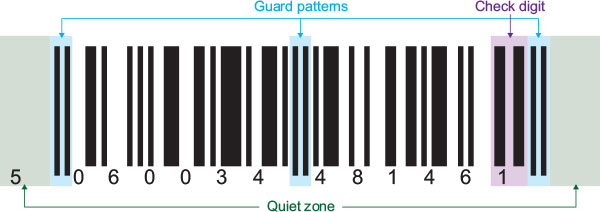
\includegraphics[width=0.8\linewidth]{obrazky-figures/basic_barcode.png}
    \caption{Části lineárního čárového kódu. Tichá zóna slouží pro snažší lokalizaci čárového kódu. Ochranný vzor ohraničuje začátek a konec čárového kódu, může však také oddělovat jeho části. Kontrolní číslice zajišťuje kontrolu integrity čárového kódu při skenování\protect\footnotemark{}.}
    \label{barcode1}
\end{figure}
\footnotetext{Dostupné z \url{https://www.cognex.com/library/media/intro-topics/intro-to-barcode-reading/fig_5_intro_to_industrial_barcode_reading-730px.jpg?h=212&w=600&la=en&hash=23466FCD5AC22EE4A74FF12C919BABDC}}

\paragraph{} Nejznámějšími lineárními čárovými kódy jsou Universal Product Codes (UPC), International Article Number (EAN) a Code 128 (obrázek \ref{lin_barcodes}).
\begin{enumerate}
    \item UPC je čistě číselný kód používaný pro spotřební zboží a to zejména v USA a Kanadě. Tyto dvanáctimístné kódy obsahují základní informace o identitě výrobce a identifikační číslo výrobku. Pozice každého čísla udává typ informace. Existuje také jednodušší varianta UPC-E která obsahuje pouze šest číslic.
    \item  Kódy EAN se podobně jako kódy UPC používají k identifikaci spotřebních výrobků, akorát ve zbytku světa. Na rozdíl od UPC, obsahuje tento formát třináct číslic. Většina prodejen snímající čárové kódy ve formátu UPC, je pak převádí na EAN. Existuje několik různých variant čárového kódu EAN, včetně EAN-13, EAN-8, JAN-13, ISBN a ISSN.
    \item  Code 128 je narozdíl od předchozích formátů osmimístný a alfanumerický. Je založen na ASCII a používá všechny jeho standardní symboly. Kódy jsou rozděleny do tří podmnožin A, B a C. Počáteční znak každého kódu označuje která podmnožina bude použita. Existují také řídíci znaky pro přepnutí na jinou podmnožinu uprostřed čárového kódu \cite{barcode_types}.
\end{enumerate}


\begin{figure}[h]\centering
    \centering
    \begin{subfigure}{0.3\textwidth}
    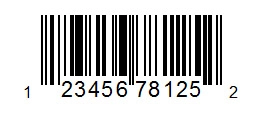
\includegraphics[width=0.9\linewidth]{obrazky-figures/UPC.png}\hfill
    \caption{UPC}
    \end{subfigure}
    \begin{subfigure}{0.3\textwidth}
    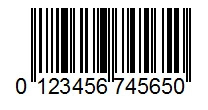
\includegraphics[width=0.9\linewidth]{obrazky-figures/EAN.png}\hfill
    \caption{EAN}
    \end{subfigure}
    \begin{subfigure}{0.3\textwidth}
    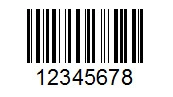
\includegraphics[width=0.9\linewidth]{obrazky-figures/code128.png}\hfill
    \caption{Code128}
    \end{subfigure}
    \caption{Typy lineárních čárových kódů\protect\footnotemark{}.}
    \label{lin_barcodes}
\end{figure}
\footnotetext{Dostupné z \url{https://barcode-labels.com/getting-started/barcodes/types/}}
\newpage
\section{Dvourozměrné čárové kódy}
\paragraph{} Na rozdíl od lineárních čárových kódů, obsahují dvourozměrné kódy informace ve vodorovném i svislém směru, což jim umožňuje uložit mnohem více dat. Například jeden 2D kód může obsahovat až 3 116 číselných znaků nebo 2 335 alfanumerických znaků, ve srovnání se třinácti znaky, které pojme EAN.
\paragraph{}
Všechny dvourozměrné kódy mají zabudovanou korekci chyb, podobně jako kontrolní číslice v některých lineárních kódech, která účinně eliminuje chybné čtení. V rámci jednoho dvourozměrného kódu jsou data obvykle zakódována třikrát, což výrazně zvyšuje šanci na správné přečtení kódu. Například u QR kódu lze získat jeho obsah při ztrátě až 7\% datových buněk.
\paragraph{}
Zatímco lineární kódy mají tiché zóny a ochranné vzory, které určují, kde kód začíná a končí, dvourozměrný kód má tichou zónu (Quiet zone), vyhledávací vzor (L pattern) a taktovací vzor (Clocking pattern), jak lze vidět v obrázku \ref{barcode2d}. Vyhledávací vzor má tvar písmene L, který se nachází kolem vnějšího okraje dvou stran dvourozměrného kódu a slouží k zajištění správné orientace při dekódování. Naproti vyhledávacímu vzoru je taktovací vzor, což řada střídajících se černých a bílých modulů (nebo buněk), které určují velikost jedné buňky a velikost kódu (počet řádků a sloupců) pro dekódování. Tichá zóna je podobná jako u lineárních čárových kódů, u dvourozměrných kódů však musí obklopovat celý kód. Existuje mnoho typů dvourozměrných čárových kódů, přičemž nejznámější jsou QR kód, PDF417 a Datová matice (obrázek \ref{2d_barcodes}) \cite{barcode1}.

\begin{figure}[h]\centering
    \centering
    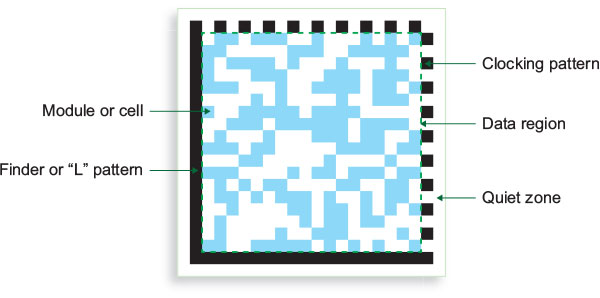
\includegraphics[width=0.8\linewidth]{obrazky-figures/barcode2D.png}
    \caption{Části dvourozměrného čárového kódu. Modul nebo buňka označuje datovou jednotku. Vyhledávací vzor slouží k zajištění správné orientace kódu. Taktovací vzor se skládá z datových regionů, které určují velikost jedné buňky a velikost samotného kódu. Tichá zóna slouží pro snažší lokaci čárového kódu, u dvourozměrných čárových kódů jej musí obklopovat celý\protect\footnotemark{}.}
    \label{barcode2d}
\end{figure}
\footnotetext{Dostupné z \url{https://www.cognex.com/library/media/intro-topics/intro-to-barcode-reading/udpate_large_2dcodebanner.jpg?h=298&w=600&la=en&hash=832766CB428519D54141D26EC524B6BE}}

\begin{enumerate}
    \item QR kódy, což je zkratka pro Quick Response kódy, jsou nejrozšířenějším dvourozměrným čárovým kódem. Je to zejména kvůli jejich širokému využití pro překlenutí propasti mezi digitálním a reálným světem. QR kód je schopen zakódovat až 2 509 číselných nebo 1 520 alfanumerických znaků a má zabudované tři úrovně detekce chyb. QR kódy mají minimální velikost 21 × 21 buněk, ale jejich velikost se může zvětšovat po 4 × 4 buňkách až do maximální velikosti 105 × 105 buněk.
    \item Kódy PDF417 jsou používaný v různých aplikacích, především v dopravě, identifikačních kartách a při správě zásob. Zkratka PDF znamená Portable Data File (přenosný datový soubor) a byla vyvinuta společností Symbol Technologies. Tento dvourozměrný kód využívá vestavěnou korekci chyb, která zajišťuje lepší čitelnost. Čárové kódy PDF417 mohou zakódovat jeden až dvě stě znaků na symbol, tedy více než jeden kilobajt dat na štítek. Čárové kódy PDF417 mají ve srovnání s ostatními dvourozměrnými čárovými kódy poněkud odlišné složení a lze jej popsat jako soubor lineárních čárových kódů naskládaných na sebe, proto se někdy označují jako naskládaná lineární symbologie.
    \item Datové matice dokážou zakódovat až 3 116 znaků z celé 256 bajtové znakové sady ASCII. Jedná se o dvourozměrný čárový kód s vysokou hustotou, který nabízí větší hustotu dat ve srovnání s čárovými kódy PDF417. Tyto čárové kódy jsou konfigurovány do čtvercové mřížky s vyhledávacím vzorem po okrajích symbolu, který umožňuje skenerům identifikovat čárový kód a přečíst jej bez ohledu na orientaci kódu. Stejně jako ostatní dvourozměrné čárové kódy obsahují Datové matice vestavěná opatření pro opravu chyb, která zajišťují integritu dat i v případě fyzického poškození kódu. Datové maticové kódy se používají především v USA a v Evropě, nejčastěji pro přímé značení dílů a laserové značení v leteckém, elektronickém a automobilovém průmyslu \cite{barcode_types}.
\end{enumerate}

\begin{figure}[h]\centering
    \centering
    \begin{subfigure}{0.3\textwidth}
    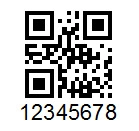
\includegraphics[width=0.9\linewidth]{obrazky-figures/QRcode.png}\hfill
    \caption{QR kód}
    \end{subfigure}
    \begin{subfigure}{0.3\textwidth}
    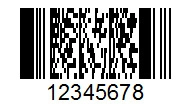
\includegraphics[width=0.9\linewidth]{obrazky-figures/PDF417.png}\hfill
    \caption{PDF417}
    \end{subfigure}
    \begin{subfigure}{0.3\textwidth}
    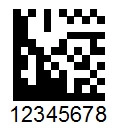
\includegraphics[width=0.9\linewidth]{obrazky-figures/datamatrix.png}\hfill
    \caption{Datová matice}
    \end{subfigure}
    \caption{Typy dvourozměrných čárových kódů. Můžeme vidět že kód PDF417 připomíná jednorozměrné čárové kódy, avšak ukládá data i vertikálně. Zbylé dva kódy jsou typickými zástupci dvourozměrných čárových kódů se svým čtvercovým tvarem\protect\footnotemark{}.}
    \label{2d_barcodes}
\end{figure}
\footnotetext{Dostupné z \url{https://barcode-labels.com/getting-started/barcodes/types/}}
\chapter{Způsoby detekce objektů v obraze}
\label{detekce_v_obraze}
\paragraph{}Systémy detekce objektů v obraze vyhledávají objekty v reálném světě pomocí předem známých modelů těchto objektů. Tento úkol je pro stroje poměrně obtížný ve srovnání s lidmi, kteří jej provádějí velmi snadno a okamžitě. V této kapitole uvedu přehled různých technik a přístupů, které se používají k detekci objektů v obrazech a videích. Konkrétně tedy metody detekce hran, metody detekce rohů, metody detekce směrové koherence a metody využívající umělé neuronové sítě.


\section{Detekce hran}
\label{detekce_hran}
\paragraph{} Hlavním cílem detekce hran je lokalizace a identifikace ostrých nespojitostí v obraze. Tyto nespojitosti jsou způsobeny náhlými změnami v intenzitě pixelů, které charakterizují hranice jednotlivých objektů. Pomocí těchto hranic můžeme identifikovat objekty za účelem rozpoznání jejich typu. Výsledky metod založených na detekci hran lze vidět na obrázku \ref{sobel_scharr}.
\paragraph{} Tato metoda používá operátory detekce hran. Tyto operátory identifikují horizontální hrany, vertikální hrany, rohové hrany a hrany se skokovou změnou intenzity. Kvalita hran detekovaných těmito operátory je vysoce závislá na šumu, světelných podmínkách, objektech stejné intenzity a hustotě hran v obraze. Tyto problémy mohou být vyřešeny úpravou různých parametrů v detektoru hran a změnou prahových hodnot pro určení hrany. 
\paragraph{} Operátory detekce hran jsou velmi citlivé na šum a hrany s vysokofrekvenčním obsahem. Proto je potřeba odstranit šum, což může vést k rozmazaným a zkresleným hranám. K dispozici je široká škála operátorů, které umožňují extrahovat hrany z obrázků různých úrovní šumu \cite{edge1}. Tyto operátory se dělí na dvě kategorie: 
\begin{enumerate}
    \item  Detekce hran na základě gradientu pracuje s první derivací intenzity obrazu. Hrana se detekuje hledáním lokálních maxim a minim. 
    Když \begin{math} I(x,y)\end{math} je vstupní obrázek, pak se gradient spočítá následovně:
    \begin{equation}
    \nabla I=\hat{x} \frac{\partial I(x, y)}{\partial x}+\hat{y} \frac{\partial I(x, y)}{\partial y}
    \end{equation}
    kde \begin{math}\frac{\partial I(x, y)}{\partial x}\end{math} je gradientem na ose \textit{x} a \begin{math}\frac{\partial I(x, y)}{\partial y}\end{math} je gradientem osy \textit{y}. 
    Vektor gradientu lze spočítat pomocí rovnice:
    
    \begin{equation}
    \nabla f=\operatorname{grad}(f)=\left[\frac{G x}{G y}\right]
    \end{equation}
    
    kde \begin{math}G_x \text{ je gradientem na ose x a } G_y\end{math} je gradientem na ose y. Velikost gradientu reprezentuje rovnice:
    \begin{equation}
    |G|=\sqrt{G x^2+G y^2}
    \end{equation}
    a směr vektoru gradientu je dán rovnicí:
    
    \begin{equation}
    \theta=\tan ^{-1}\left[\frac{G y}{G x}\right]
    \end{equation}
    
    Přístup založený na gradientu využívá masky a operátory. Maska je matice, kterou aplikujeme na obraz a operátor je matematický výraz, který se aplikuje na obraz pomocí masky. Existuje mnoho takových masek a operátorů, například Sobelův operátor a Scharrův operátor \cite{edge_types}.
    
    \item Detekce hran pomocí Laplaceova operátoru definuje diskrétní formulaci derivace druhého řádu, na základě níž konstruuje filtr. V případě Laplaceova operátoru nás v podstatě zajímá konstrukce izotropních filtrů.
    \paragraph{} Izotropní filtr je takový filtr, který je invariantní vůči rotaci, což znamená, že při použití filtru tak jak je a následném použití filtru otočeného o 90° je výsledek stejný. Nejjednodušší izotropní derivací je Laplacián, který lze znázornit jako funkci dvou proměnných, reprezentující obraz, následující rovnicí:

    \begin{equation}
    \nabla^2 f=\frac{\partial^2 f}{\partial x^2}+\frac{\partial^2 f}{\partial y^2}
    \end{equation}
    kde \textit{f} reprezentuje filtr a \textit{x} a \textit{y} reprezentují osy obrazu. Mezi metody založené na Laplaceově operátoru patří například Marr-Hildreth operátor \cite{edge_types}.

\end{enumerate}


\subsection*{Sobelův operátor}
\paragraph{} Sobelův operátor je dvojicí konvolučních jáder o rozměrech 3x3. Jedno jádro je určeno pro horizontální změny a druhé, otočené o 90°, pro vertikální změny. Tyto jádra jsou reprezentovány následujícími maticemi:
\begin{equation}
\mathrm{G}_{\mathrm{x}}=\left[\begin{array}{lll}
-1 & 0 & +1 \\
-2 & 0 & +2 \\
-1 & 0 & +1
\end{array}\right] \quad \mathrm{G}_{\mathrm{y}}=\left[\begin{array}{ccc}
+1 & +2 & +1 \\
0 & 0 & 0 \\
-1 & -2 & -1
\end{array}\right]
\end{equation}

Sobelovy masky jsou navrženy tak, aby maximálně reagovaly na hrany probíhající vertikálně a horizontálně vzhledem k pixelové mřížce. Tyto směrové hrany jsou nakonec kombinovány pro určení absolutní hodnoty a směru gradientu. Sobelův operátor používá pouze celočíselné hodnoty koeficientů pro vážení a aproximaci gradientu obrazu \cite{sobel}.

\subsection*{Scharrova metoda detekce}
\label{scharr}
\paragraph{}Scharrovva metoda detekce v obraze je variantou Sobelova operátoru, který se běžně používá k detekci hran v obraze. Scharrův operátor používá jádro 3x3 k výpočtu gradientu intenzity obrazu v každém pixelu. Jádro je navrženo tak, aby bylo více rotačně symetrické než Sobelův operátor, což může být užitečné pro detekci hran pod jinými úhly než 0, 45, 90 nebo 135 stupňů. Scharrův operátor má dvě jádra: jedno pro detekci horizontálních hran a druhé pro detekci vertikálních hran. Tyto jádra vypadají následovně:
\begin{equation}
\mathrm{G}_{\mathrm{x}}=\left[\begin{array}{lll}
-3 & 0 & +3 \\
-10 & 0 & +10 \\
-3 & 0 & +3
\end{array}\right] \quad \mathrm{G}_{\mathrm{y}}=\left[\begin{array}{ccc}
-3 & -10 & -3 \\
0 & 0 & 0 \\
3 & 10 & 3
\end{array}\right]
\end{equation}
\paragraph{} Jádro se konvoluje s obrazem tak, že se střed jádra přesune nad každý pixel obrazu a hodnoty jádra se vynásobí odpovídajícími hodnotami pixelů. Výsledné hodnoty se pak sečtou a pomocí tohoto součtu lze získat velikost (rovnice \ref{magnitude_scharr}) a orientaci (rovnice \ref{orientation_scharr}) gradientu v daném pixelu.

\begin{equation}\label{magnitude_scharr}
G = \sqrt{G_x^2 + G_y^2}
\end{equation}

\begin{equation}\label{orientation_scharr}
\theta = \operatorname{arctan2}(G_y, G_x)
\end{equation}



Tento gradient vyjadřuje jak rychle se mění intenzita obrazu v horizontálním a vertikálním směru. Vysoké hodnoty gradientu označují silné hrany v obraze, zatímco nízké hodnoty označují hladké oblasti \cite{scharr}.

\begin{figure}[h]\centering
    \centering
    \begin{subfigure}{0.3\textwidth}
    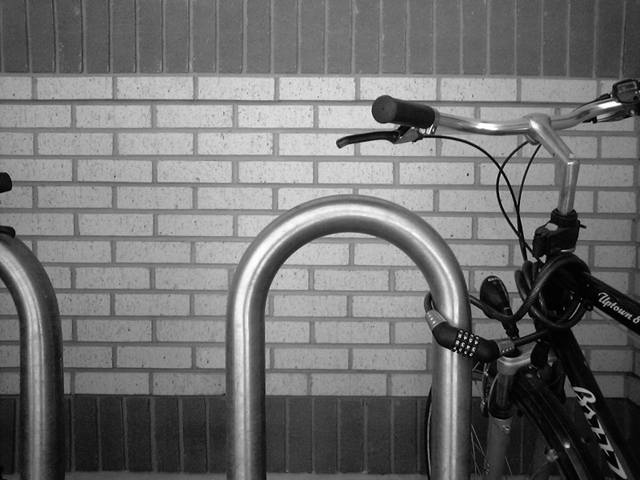
\includegraphics[width=0.9\linewidth]{obrazky-figures/edge_original.png}\hfill
    \caption{Originál}
    \end{subfigure}
    \begin{subfigure}{0.3\textwidth}
    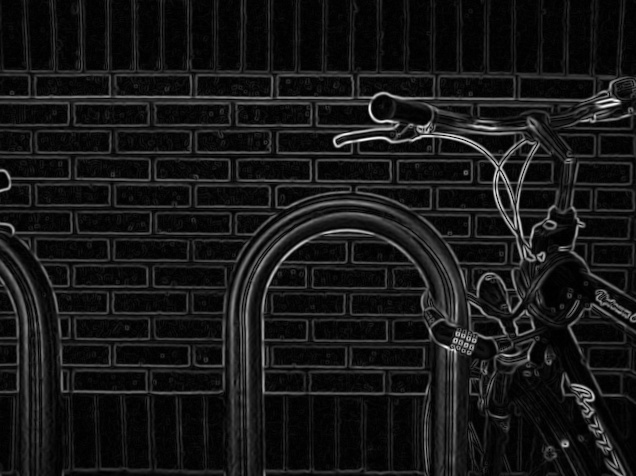
\includegraphics[width=0.9\linewidth]{obrazky-figures/edge_sobel.png}\hfill
    \caption{Sobel}
    \end{subfigure}
    \begin{subfigure}{0.3\textwidth}
    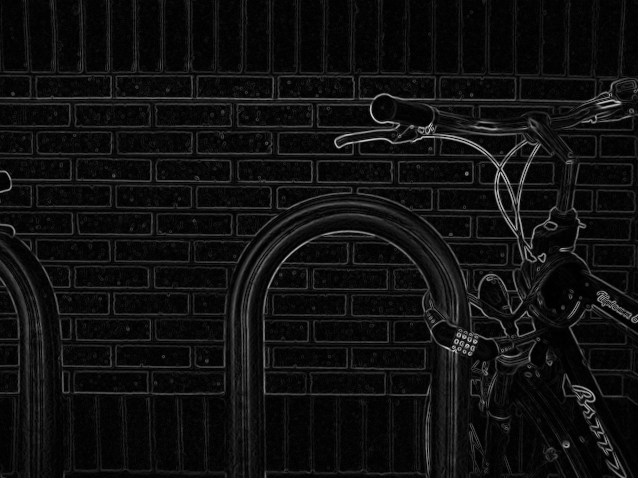
\includegraphics[width=0.9\linewidth]{obrazky-figures/edge_scharr.png}\hfill
    \caption{Scharr}
    \end{subfigure}
    \caption{Porovnání Sobelovy a Scharrovy metody\protect\footnotemark{}.}
    \label{sobel_scharr}
\end{figure}
\footnotetext{Dostupné z \url{https://en.wikipedia.org/w/index.php?title=Sobel_operator&oldid=1152249844}}
\section{Detekce rohů}
\label{detekce_rohu}
\paragraph{} Detekce rohů je nízkoúrovňová technika zpracování obrazu, která je široce používaná v různých aplikacích počítačového vidění jako je kalibrace kamery, sledování cílů, identifikace transformovaného obrazu, registrace obrazů, 3D modelování budov z leteckých snímků, extrakce příznaků dat LIDAR na více měřítkách nebo extrakce budov 2D a 3D. Nicméně různé přístupy vyžadují odlišný pohled na definici rohů. Historicky se termín rohový bod odkazoval jak na zájmový bod, tak na zájmovou oblast. Obecně se detekce rohů v obraze vztahuje k bodu na obrysu, kde se setkávají dvě přímé hrany pod určitým úhlem, nebo k lokaci, kde se významně mění směr obrysu. Výstup typického detektoru rohů lze vidět na obrázku \ref{corner}.

Existující metody detekce rohů mohou být rozděleny do dvou kategorií: detektory založené na intenzitě a detektory založené na obrysech \cite{s140304126}. Příklady detekce těchto detektorů je možno vidět na obrázku \ref{css_harris}.

\begin{figure}[h]\centering
    \centering
    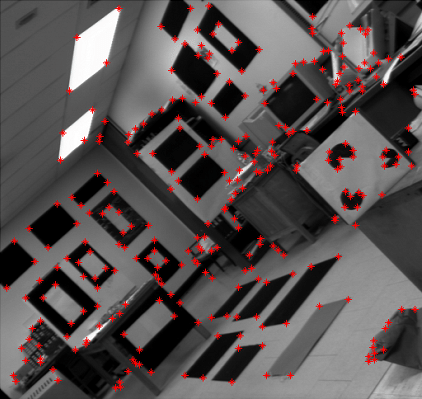
\includegraphics[width=0.6\linewidth]{obrazky-figures/corner.png}
    \caption{Výstup typického detektoru rohů\protect\footnotemark{}.}
    \label{corner}
\end{figure}
\footnotetext{Dostupné z \url{https://www.mdpi.com/1424-8220/14/3/4126}}
\subsection*{Detektory založené na intezitě}
\paragraph{}Hans Moravec \cite{Moravec} definoval roh jako bod, kde byla pozorována silná změna dvoudimenzionální intenzity jasu ve všech směrech. Na základě této definice Moravec vytvořil jeden z prvních detektorů rohů. Z tohoto detektoru se postupně vyvinuly všechny moderní detektory rohů založené na intenzitě obrazu \cite{intensity_corner}. Jeden z nejpopulárnějších detektorů rohů který se používá dodnes je Harrisův detektor.

\subsection*{Harris corner detector}
\label{harrisc}
Harrisův detektor rohů je založen na druhém řádu matice derivací funkce obrazu v každém bodě daného obrazu. Druhý řád matice popisuje lokální změny signálu s okny posunutými o malou vzdálenost v různých směrech. V připadě rohového bodu se intenzita obrazu bude výrazně měnit při posunu okna libovolným směrem. Hodnoty Harrisovy matice \textit{M} jsou úzce spojeny s derivacemi intenzity obrazu a jsou definovány následovně:
\begin{equation}\label{harrismatrix}
M(\mathbf{x})=\sum_{x, y} w(x, y)\left[\begin{array}{cc}
I_x^2(\mathbf{x}) & I_x I_y(\mathbf{x}) \\
I_x I_y(\mathbf{x}) & I_y^2(\mathbf{x})
\end{array}\right]
\end{equation}
kde \begin{math}I_x(\mathbf{x})\end{math} a \begin{math}I_y(\mathbf{x})\end{math} jsou derivací intenzity pixelů ve směru \textit{x} a \textit{y} v bodě \begin{math}\mathbf{x}\end{math}. Okno \textit{w(x,y)} je umístěno na pozici \textit{(x,y)}. Vlastní hodnoty matice \textit{M} mohou pomoci k určení vhodnosti okna díky této rovnice:
\begin{equation}
R=\operatorname{det} M-k(\operatorname{trace} M)^2
\end{equation}
Hodnota \textit{R} zde reprezentuje onu vhodnost okna a je počítána pro každé okno, kde \begin{math}
\operatorname{det} M=\lambda_1 \lambda_2 \text {, }\text { trace } M=\lambda_1+\lambda_2 \text { a } k
\end{math} je konstantou. Obvyklou hodnou této konstanty je 0.04. Všechna okna s hodnotou \textit{R} přesahující zadaný práh jsou považovány za rohy \cite{harris}.






\subsection*{Detektory založené na obrysech}
\paragraph{} Detekční techniky založené na obrysech obvykle zahrnují pět kroků: detekci hran, výběr kontur, vyhlazení křivky, odhad křivosti a hledání rohů. Pokud jde o metody detekce rohů založené na obrysech, jsou rohy považovány za body s lokální absolutně maximální křivostí na vybraných obrysech. Proto je odhad digitální křivosti v rovině klíčovým krokem pro detektory rohů založené na obrysech \cite{contourdetection}.
\subsection*{Curvature scale space} 
\label{curv}
\paragraph{}Metoda Curvature scale space \cite{css} je nejklasičtějším zástupcem detektorů založených na obrysech. Rohy jsou zde definovány jako lokální maxima absolutní hodnoty křivosti. Při velmi nízké míře vyhlazení v obrázku existuje mnoho takových maxim, které jsou způsobeny šumem na digitálním obrysu. Při zvětšení míry vyhlazení šum mizí a zůstávají pouze maxima odpovídající skutečným rohům. Metoda detekce Curvature scale space najde rohy v těchto lokálních maximech.
\paragraph{} Jak se obrys vyvíjí, skutečné polohy rohů se mění. Pokud se detekce provádí s velkou mírou vyhlazení, lokalizace rohů může být neuspokojivá. Aby se předešlo tomuto problému, zavádí se detekce se sledováním. Rohy jsou lokalizovány na obrázcích s velkou mírou vyhlazení, čímž se zajistí, že detekce rohů není ovlivněna šumem. Míra vyhlazení se poté redukuje a ty stejné, již detekované rohy jsou zkoumány při těchto nižších mírách vyhlazení. Výsledkem je aktualizace poloh rohů. Toto pokračuje, dokud není míra vyhlazení velmi nízká a operace velmi lokální. Tím se zvýší lokalizace i přes nízké výpočetní náklady. Ty jsou nízké, protože hodnoty křivosti při nižší míře vyhlazení nemusí být vypočteny v každém bodě obrysu, ale pouze v malém okolí detekovaných rohů.
\paragraph{} Na vyvinutých obrysech se můžou vyskytovat lokální maxima z důvodu rohů s nízkým zakřivením nebo šumu. Ty mohou být odstraněny zavedením prahové hodnoty \textit{T}. Tato adaptivní prahová hodnota lze vypočítat následovně:
\begin{equation}\label{contourequation}
T(u)=C \times \bar{K}=1.5 \times \frac{1}{L 1+L 2+1} \sum_{i=u-L .2}^{u+L 1} \kappa(i)
\end{equation}
kde \textit{C} je koeficient, \begin{math}\bar{K}\end{math} reprezentuje střední hodnotu křivosti oblasti \textit{u}. \textit{L1} a \textit{L2} jsou velikosti této oblasti. Pokud je křivost kandidátního rohu menší než prahová hodnota, jedná se o zaoblený roh a bude odstraněn. Je třeba podotknout že pokud je C nastaveno na 1, žádný roh není odstraněn. Pokud je C nastaveno na 2, roh který splňuje rovnici \ref{contourequation} je standardní trojúhelník. Teoreticky by tedy \textit{C} mělo být nastaveno na hodnotu mezi 1 a 2 \cite{cssequation}.
\pagebreak

\begin{figure}[h]\centering
    \centering
    \begin{subfigure}{0.45\textwidth}
    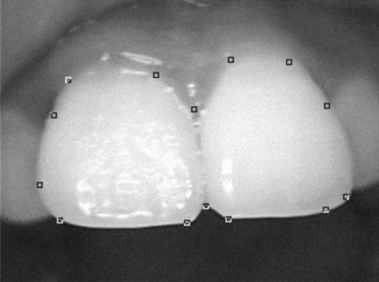
\includegraphics[width=0.9\linewidth]{obrazky-figures/css2.png}\hfill
    \caption{CSS detektor}
    \end{subfigure}
    \begin{subfigure}{0.45\textwidth}
    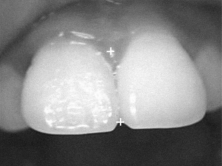
\includegraphics[width=0.9\linewidth]{obrazky-figures/harris1.png}\hfill
    \caption{Harrisův detektor s thresholdem 5000}
    \end{subfigure}
    \begin{subfigure}{0.45\textwidth}
    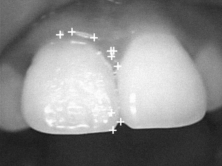
\includegraphics[width=0.9\linewidth]{obrazky-figures/harris2.png}\hfill
    \caption{Harrisův detektor s thresholdem 2000}
    \end{subfigure}
    \begin{subfigure}{0.45\textwidth}
    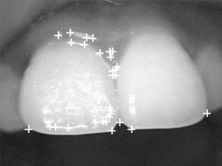
\includegraphics[width=0.9\linewidth]{obrazky-figures/harris3.png}\hfill
    \caption{Harrisův detektor s thresholdem 1000}
    \end{subfigure}
    \caption{Porovnání CSS a Harrisovy metody. Lze vidět měnící se počet detekovaných rohů Harrisovou metodou v závislosti na hodnotě prahu. Také jde pozorovat detekce změn jasu Harrisova detektoru v důsledku odrazu světla od zubu zejména při nižších hodnotách prahu\protect\footnotemark{}.}
    \label{css_harris}
\end{figure}
\footnotetext{Dostupné z \url{https://ieeexplore.ieee.org/document/5609958/figures##figures}}


\section{Detekce směrové koherence}
Směrová koherence je vlastnost světelných vln, která popisuje stupeň korelace mezi dvěma světelnými vlnami šířícími se v různých směrech. Sama o sobě není typem detekce obrazu, ale lze ji využít i v technikách zpracování obrazu\cite{kim2017directional}.


\subsection*{Detektor čárových kódů knihovny OpenCV}
\label{opencv}
\paragraph{}Tato metoda původně vznikla pro detekci otisku prstů, ale má i jiné způsoby využití, například právě pro detekci čárových kódů \cite{opencv_barcode}. 

Nejprve vypočítá průměrný čtvercový gradient každého pixelu, ať už je to singulární bod nebo nikoliv. Singulární body jsou body, kde je směrové pole nespojité. V ridge-valley strukturách jsou definovány dva typy těchto singulárních bodů, jádro a delta. Jádro je nejvyšším bodem zakřivení hřebene, zatímco delta je středem trojúhelníkových oblastí, kde se setkávají tři různé směry proudění. Kromě své lokace mají tyto body také orientaci. Směrové pole popisuje hrubou strukturu, nebo základní tvar obrazu a je definováno jako lokální orientace ridge-valley struktur. Příklad směrového pole a singulárních bodů lze vidět v obrázku \ref{directional_singular}. Metoda může detekovat dva různé body jen pár pixelů od sebe. Je třeba dbát na to, aby směrová pole s vysokým rozlišením byla dostatečně zprůměrována tak, aby byly předem eliminovány falešné body. Algoritmus pro extrakci těchto bodů totiž detekuje všechny singulární body v poli s daným rozlišením.

\begin{figure}[h]\centering
    \centering
    \begin{subfigure}{0.3\textwidth}
    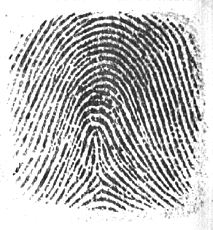
\includegraphics[width=0.9\linewidth]{obrazky-figures/fingerprint1.png}\hfill
    \caption{Otisk prstu}
    \label{ds_a}
    \end{subfigure}
    \begin{subfigure}{0.3\textwidth}
    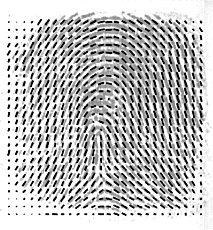
\includegraphics[width=0.9\linewidth]{obrazky-figures/fingerprint2.png}\hfill
    \caption{Směrové pole}
    \label{ds_b}
    \end{subfigure}
    \begin{subfigure}{0.3\textwidth}
    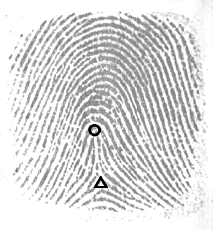
\includegraphics[width=0.9\linewidth]{obrazky-figures/fingerprint3.png}\hfill
    \caption{Singulární body}
    \label{ds_c}
    \end{subfigure}
    \caption{V obrázku \ref{ds_b} lze vidět směrové pole otisku prstu, ze kterého jdou vyčíst také singulární body. Ty jsou ukázány v obrázku \ref{ds_c}, kde kolečko reprezentuje jádro a trojúhelník bod delta\protect\footnotemark{}.}
    \label{directional_singular}
\end{figure} 
\footnotetext{Dostupné z \url{https://ieeexplore.ieee.org/document/1017618/figures##figures}}
Tento algoritmus vezme na vstupu čtvercové směrové pole a vypočítá gradientní vektor \textit{J} pomocí této rovnice:
\begin{equation}
\left[\begin{array}{l}
J_x(x, y) \\
J_y(x, y)
\end{array}\right]=\nabla 2 \theta(x, y)=\left[\begin{array}{l}
\frac{\partial 2 \theta(x, y)}{\partial x} \\
\frac{\partial \partial(x, y)}{\partial y}
\end{array}\right]
\end{equation}
Kde \begin{math}2 \theta(x, y)\end{math} reprezentuje orientaci čtvercového směrového pole (obrázek \ref{gradient_directional}).
Při výpočtu diskrétní verze tohoto gradientu by se měly obě složky \textit{J} počítat jako modulo \begin{math}2\pi\end{math} tak, aby byly vždy mezi hodnotami \begin{math}-\pi \text{ a } \pi\end{math}, čímž se orientace stane cyklickou.

\begin{figure}[h]\centering
    \centering
    \begin{subfigure}{0.45\textwidth}
    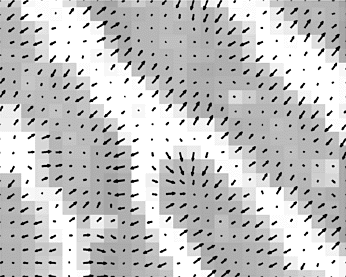
\includegraphics[width=0.9\linewidth]{obrazky-figures/gradient1.png}\hfill
    \caption{Gradient}
    \label{gd_a}
    \end{subfigure}
    \begin{subfigure}{0.45\textwidth}
    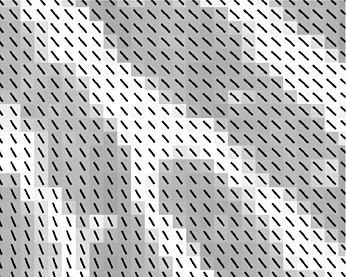
\includegraphics[width=0.9\linewidth]{obrazky-figures/gradient2.png}\hfill
    \caption{Zprůměrované směrové pole}
    \label{gd_b}
    \end{subfigure}
    \caption{Na obrázku \ref{gd_a} lze vidět gradient otisku prstu, neboli směr ve kterém nastává největší změna intenzity v daném bodě. Obrázek \ref{gd_b} ukazuje směr detekovaných struktur otisku prstu\protect\footnotemark{}.}
    \label{gradient_directional}
\end{figure}
\footnotetext{Dostupné z \url{https://ieeexplore.ieee.org/document/1017618/figures##figures}}

\paragraph{}
Dalším krokem je aplikace Greenova teorému \cite{directional}, který říká, že uzavřený lineární integrál nad vektorovým polem lze vypočítat jako plošný integrál nad rotací pole tohoto vektorového pole:
\begin{equation}
\begin{aligned}
\oint_{\partial A} w_x d x+w_y d y & =\iint_A \operatorname{rot}\left[w_x w_y\right]^T d x d y \\
& =\iint_A\left(\frac{\partial w_y}{\partial x}-\frac{\partial w_x}{\partial y}\right) d x d y
\end{aligned}
\end{equation}
kde \textit{x} a \textit{y} definují koordinovaný systém, \textit{A} je oblast a \begin{math}\theta A\end{math} je obrysem kolem této oblasti. \begin{math}\operatorname{rot}\left[w_x w_y\right]^T\end{math} reprezentuje vektorové pole. Tento teorém se aplikuje na součet gradientů čtvercové orientace na obrysu:
\begin{equation}
\begin{aligned}
\text { Index } & =\sum_{\Delta x, \Delta y \text { along } \partial A}\left(J_x \cdot \Delta x+J_y \cdot \Delta y\right)=\sum_A \operatorname{rot}\left[J_x J_y\right]^T \\
& =\sum_A\left(\frac{\partial J_y}{\partial x}-\frac{\partial J_x}{\partial y}\right) .
\end{aligned}
\end{equation}
Protože všechny singulární body musí být extrahovány ze směrového pole, \textit{A} se vezme jako čtverec o velikosti jednoho pixelu. To vede k velmi efektivní metodě výpočtu Poincareova indexu \cite{directional}. Poincarého index \cite{poincare} slouží k měření toho, jak se vektorové pole na uzavřené ploše ovíjí kolem singulárního bodu (obrázek \ref{gradient_points}).

\paragraph{}
Narozdíl od jiných metod extrakce singulárního bodu, má jádrový bod za následek hodnotu Poicarého indexu \begin{math}2 \pi\end{math}, bod delta hodnotu \begin{math}- 2 \pi\end{math}, zatímco index ostatních pixelů se rovná nule. Přesná lokace singulárního bodu ve směrovém poli se nachází mezi těmito dvěma pixeli. Tato metoda detekuje body ve všech sousedních pixelech žádaného bodu, kvůli oblasti podpory gradientího oparátoru \cite{directional}.

\begin{figure}[h]\centering
    \centering
    \begin{subfigure}{0.45\textwidth}
    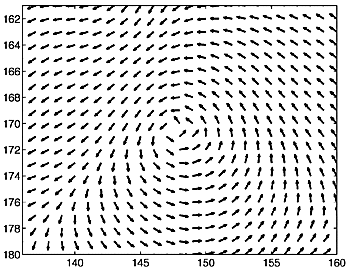
\includegraphics[width=0.9\linewidth]{obrazky-figures/gradient_table1.png}\hfill
    \caption{Jádrový bod}
    \end{subfigure}
    \begin{subfigure}{0.45\textwidth}
    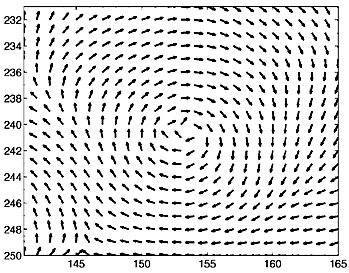
\includegraphics[width=0.9\linewidth]{obrazky-figures/gradient_table2.png}\hfill
    \caption{Bod delta}
    \end{subfigure}
    \caption{Gradienty čtvercových směrových polí ovíjející se kolem singulárních bodů\protect\footnotemark{}.}
    \label{gradient_points}
\end{figure}
\footnotetext{Dostupné z \url{https://ieeexplore.ieee.org/document/1017618/figures##figures}}


\section{Neuronové sítě}
\label{neural_networks}
\paragraph{} 
Umělé neuronové sítě jsou výpočetní systémy zpracování dat, které jsou do značné míry inspirovány fungováním biologických nervových systémů. Tyto sítě se většinou skládají z velkého počtu vzájemně propojených vypočetních uzlů označovaných jako neurony. Tyto uzly pracují propojeně distribuovaným způsobem, aby se společně učily ze vstupů s cílem optimalizovat svůj konečný výstup.
\paragraph{}
Základní strukturu umělé neuronové sítě lze modelovat podle obrázku \ref{simple_neural}. Vstupní data, obvykle ve formě vícerozměrného vektoru, neboli tenzoru, jsou vložena do vstupní vrstvy, která je rozdělí do skrytých vrstev. Skryté vrstvy pak budou rozhodovat na základě předchozí vrstvy a zvažovat, jak stochastická změna v této vrstvě poškodí nebo zlepší finální výstup, což se označuje jako proces učení. Mít více skrytých vrstev naskládaných na sobě se běžně nazývá hluboké učení.

\begin{figure}[h]\centering
    \centering
    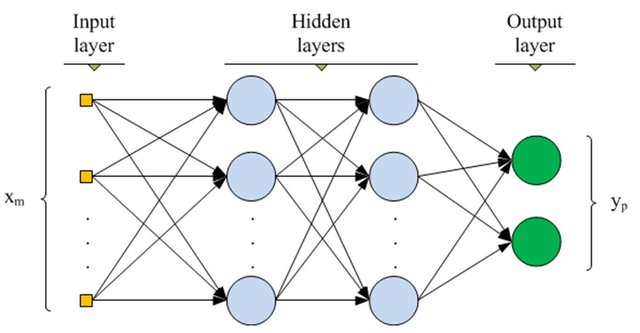
\includegraphics[width=0.6\linewidth]{obrazky-figures/simple_neural.png}
    \caption{Jednoduchá neuronová síť s input vrstvou, skrytými vrstvami a output vrstvou\protect\footnotemark{}.}
    \label{simple_neural}
\end{figure}
\footnotetext{Dostupné z \url{https://www.researchgate.net/profile/Vincenzo-Lomonaco/publication/285583518/figure/fig3/AS:375714613350403@1466588752867/Multilayer-Perceptron-commonly-used-architecture-14_W640.jpg}}
\paragraph{}
Dvěmi klíčovými paradigmaty učení v úlohách zpracování obrazu, jsou učení s učitelem a učení bez učitele. Učením s učitelem se označuje postup, kdy jsou definováný předem označené vstupy, které slouží jako cíle. Pro každý trénovací příklad musí existovat sada vstupních hodnot (vektorů) a jedna nebo více souvisejících určených výstupních hodnot. Cílem této formy učení je snížit celkovou chybu klasifikace modelů, a to prostřednictvím správného výpočtu výstupní hodnoty tréninkového příkladu. Obecnou rovnicí trénování neuronových sítí je:

\begin{equation}
\theta^{t+1}=\theta^t-\alpha \frac{\partial E\left(X, \theta^t\right)}{\partial \theta}
\end{equation}
kde \begin{math}\alpha\end{math} značí míru učení a \begin{math} E\left(X, \theta\right)\end{math} představuje chybovou funkci. \begin{math}\theta^t\end{math} reprezentuje parametr neuronové sítě v iteraci \textit{t} algoritmu Gradient descent. Chybová funkce definuje chybu mezi očekávaným výstupem a výstupem neuronové sítě. Gradientní descent je optimalizační algoritmus který slouží k nalezení lokálního maxima nebo minima dané funkce \cite{brilliant-backpropagation}.

\paragraph{}
Naproti tomu učení bez učitele je typ strojového učení, při kterém je algoritmus trénován na neoznačeném souboru dat. To znamená, že soubor dat použitý k trénování obsahuje pouze vstupní data bez odpovídajících výstupních hodnot nebo značek. Během trénování se algoritmus snaží identifikovat vzory nebo struktury ve vstupních datech, aniž by mu bylo výslovně řečeno, jaké tyto vzory nebo struktury mají být \cite{neural1}.
\paragraph{}
Specifickým typem umělých neuronových sítí jsou konvoluční neuronové sítě. Jsou to specializovanou formou hlubokých neuronových sítí pro analýzu vstupních dat, která obsahují určitou formu prostorové struktury. Tyto sítě jsou využívány primárně k řešení problémů týkající se počítačového vidění.
\subsection*{Tenzory}
Všechny současné algoritmy strojového učení používají jako základní datovou strukturu tenzory. Příklad takového tenzoru lze vidět v obrázku \ref{rgb_tensor}. Tenzory mají ve strojovém učení zásadní význam. Rozumíme jimi zobecnění vektorů a matic na libovolný počet dimenzí. Tenzory se dělí podle jejich rozměru (počtu os) na 0D tenzory, 1D tenzory, 2D teznory, 3D tenzory a 4D tenzory. Čili 3D tenzor obsahuje osy x, y a z. Je to tedy několik tabulek se sloupci a řádky. 4D tenzor vznikne při umístění několika 3D tenzorů do řetězce \cite{neural2}.

\begin{figure}[h]\centering
    \centering
    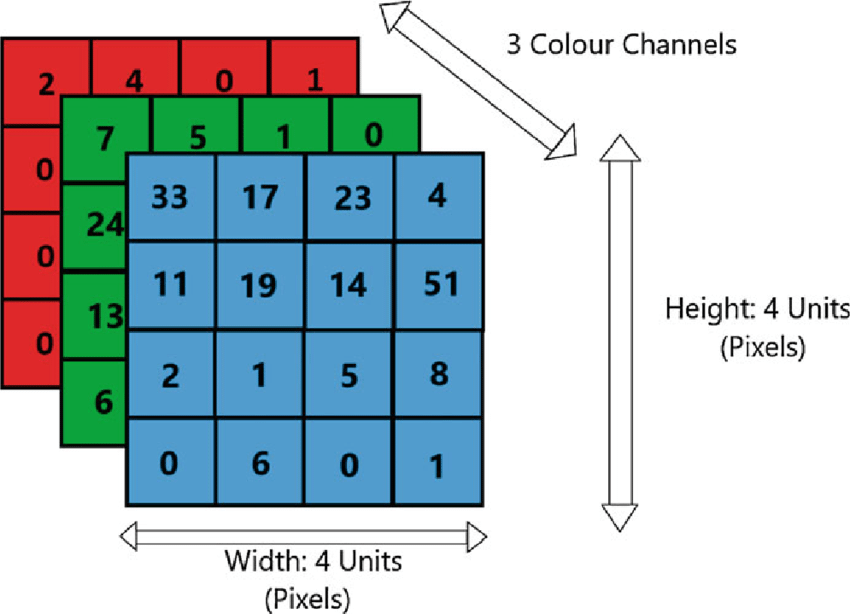
\includegraphics[width=0.9\linewidth]{obrazky-figures/tensor.png}
    \caption{Příklad 3D tenzoru ukládajícího Red-Green-Blue (RGB) obrázek\protect\footnotemark{}.}
    \label{rgb_tensor}
\end{figure}
\footnotetext{Dostupné z \url{https://www.researchgate.net/profile/Osval-Montesinos-Lopez/publication/357820593/figure/fig2/AS:1134626982625284@1647527561324/A-3D-tensor-of-a-Red-Green-Blue-RGB-image-of-a-dimension-of-4-A-4-A-3_W640.jpg}}

\subsection*{Konvolučních neuronové sítě}
\paragraph{}Jak již bylo uvedeno dříve, konvoluční neuronové sítě se primárně zaměřují na to, že vstupní data budou tvořena obrázky. Proto je třeba architekturu nastavit tak, aby co nejlépe vyhovovala potřebě pracovat s daným typem dat.
Jedním z klíčových rozdílů je, že neurony, které vrstvy v rámci konvolučních neuronových sítí tvoří, jsou složeny z neuronů uspořádaných do tří dimenzí: prostorové dimenzionality vstupu (výška a šířka) a hloubky. Hloubka neznamená celkový počet vrstev v rámci umělé neuronové sítě, ale třetí rozměr aktivačního objemu. Každý neuron v konvoluční vrstvě je propojen pouze s malou oblastí vrstvy před ní, což umožňuje efektivní využití paměti a urychluje výpočet.

\paragraph{}
Konvoluční neuronové sítě obsahují tři základní typy vrstev. Jedná se o konvoluční vrstvy, pooling vrstvy a plně propojené vrstvy. Když se tyto vrstvy poskládají na sebe, vznikne architektura konvolučních neuronových sítí. Zjednodušená architektura těchto sítí pro klasifikaci MNIST je znázorněna na obrázku \ref{cnn1}. Základní funkce výše uvedeného příkladu konvoluční sítě lze rozdělit do tří klíčových oblastí:

\begin{enumerate}
    \item Konvoluční vrstva určuje výstup neuronů, které jsou připojeny k lokálním oblastem vstupu, pomocí výpočtu skalárního součinu mezi jejich váhami a oblastí připojenou ke vstupnímu objemu (obrázek \ref{conv}). Rektifikovaná lineární jednotka (běžně zkracovaná na ReLu) \cite{relu} je aktivační funkce využívaná v neuronových sítích pro zvýšení nonlinearit a zlepšení výkonu sítě. Nonlinearita je vlastnost systému, která znamená, že jeho odezva na vstupní signál není úměrná velikosti tohoto signálu. Funkce ReLu je jednoduchá a rychlá na výpočet, protože při záporných vstupech je výstup neuronů roven nule, jinak je roven jeho vstupu. Tato funkce se hojně používá například při detekci objektů v obraze nebo při rozpoznávání řeči.  
\begin{figure}[ht]\centering
    \centering
    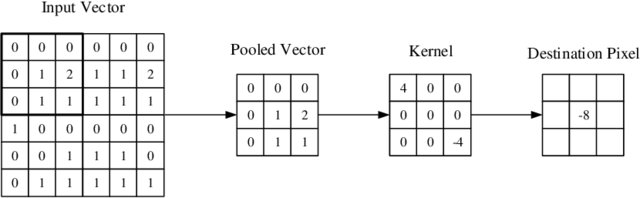
\includegraphics[width=0.6\linewidth]{obrazky-figures/convolution.png}
    \caption{Vizuální reprezentace konvoluce. Jádro je umístěno nad vstupní vektor a s jeho pomocí se vypočítá vážená suma všech pixelů pod tímto jádrem\protect\footnotemark{}.}
    \label{conv}
\end{figure}
\footnotetext{Dostupné z \url{https://www.researchgate.net/profile/Keiron-Oshea/publication/285164623/figure/fig6/AS:667895520575488@1536250109021/A-visual-representation-of-a-convolutional-layer-The-centre-element-of-the-kernel-is_W640.jpg}}
\item Pooling vrstva provádí downsampling podél prostorové dimenzionality daného vstupu, čímž dále snížuje počet výstupů v rámci dané aktivace \cite{neural1}.
\item Úplně propojená vrstva vrstva se snaží z aktivací vytvořit skóre tříd, které se použije pro klasifikaci. Navrhuje se také, aby mezi těmito vrstvami byla použita aktivační funkce ReLu. Bez aktivační funkce by síť zkolabovala do jedné vrstvy a nebyla by schopna řešit složitější úlohy.
\end{enumerate}
\paragraph{}
Prostřednictvím těchto vrstev jsou konvoluční neuronové sítě schopny transformovat původní vstup pomocí konvolučních a downsamplingových technik a vytvářet skóre tříd pro účely klasifikace a regrese \cite{neural1}.

\pagebreak
\subsection*{Architektura YOLO}
\paragraph{} Modely rodiny You Only Look Once neboli YOLO \cite{yolo1} jsou rychlejší než modely rodiny R-CNN, takže se obvykle používají v různých úlohách v reálném čase, například při detekci objektů ve videozáznamech. Tato rychlost je dána zejména tím, že model YOLO používá takzvaný one-stage detekční algoritmus. Což znamená že YOLO detekuje v celém obraze najednou. Model R-CNN používa two-stage algoritmus, tedy nejprve detekuje zájmové oblasti a až poté hledané objekty \cite{rcnn-yolo}.
\begin{figure}[h]\centering
    \centering
    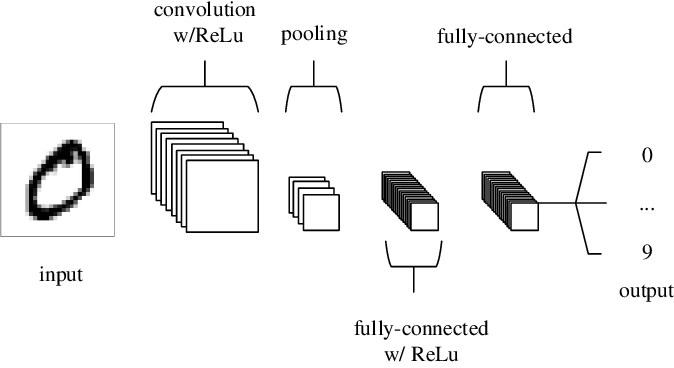
\includegraphics[width=0.8\linewidth]{obrazky-figures/cnn1.png}
    \caption{Jednoduchá architektura konvoluční neuronové sítě. Z obrázku vyplývá pořadí vrstev v konvolučních neuronových sítích. Také lze vidět plně propojenou vrstvu s aktivační funkcí ReLu\protect\footnotemark{}.}
    \label{cnn1}
\end{figure}
\footnotetext{Dostupné z \url{https://www.researchgate.net/profile/Keiron-Oshea/publication/285164623/figure/fig4/AS:667895516377100@1536250108959/An-simple-CNN-architecture-comprised-of-just-five-layers_W640.jpg}}
\paragraph{}
Jádro algoritmu detekce cílů YOLO spočívá v malé velikosti modelu a rychlosti výpočtu. Struktura této sítě je poměrně jednoduchá. Původní architektura YOLO se skládá z 24 konvolučních vrstev, za nimiž následují dvě plně propojené vrstvy. Může přímo detekovat polohu a kategorii ohraničujícího boxu (anglicky bounding box) prostřednictvím neuronové sítě. Výhodou YOLO je, že dokáže pracovat s celým obrazem najednou a tím zachytit globální informace, což umožňuje rychlejší a účinnější detekci objektů v obraze. Dokáže se také naučit vysoce zobecněné funkce, což umožňuje přenášet naučené znalosti do jiných oblastí.
\paragraph{}
Výsledky testů YOLO jsou špatné v případě objektů, které jsou velmi blízko sebe a ve skupinách. Tento špatný výkon je způsoben metodou Non-Maximum Supression, která potlačuje překrývající se ohraničující boxy a eliminuje detekci s nízou pravděpodobností. Pokud jsou dva ohraničující boxy s vysokou pravděpodobností dostatečně blízko u sebe, Non-Maximum Supression vybere nejpravděpodobnější detekci a zbytek potlačí.
\paragraph{}
YOLO má dvě vady, první je nepřesné určení polohy a druhou je nižší hodnota metriky recall. Novější verze YOLO se proto zlepšují především v těchto dvou aspektech \cite{yolo2}.
\pagebreak
\begin{figure}[h]\centering
    \centering
    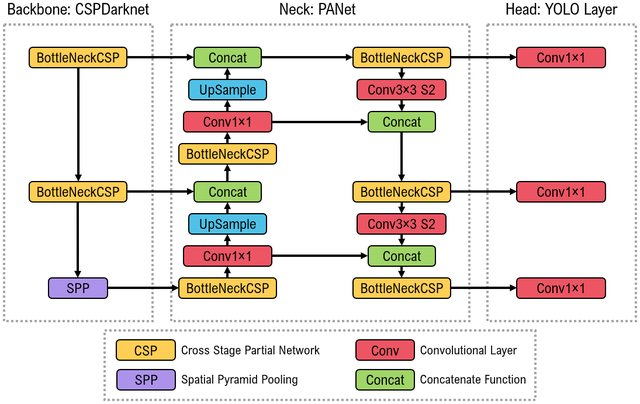
\includegraphics[width=0.8\textwidth]{obrazky-figures/yolo_overview.png}
    \caption{Architektura modelu YOLOv5, se skládá ze tří částí: páteř (CSPDarknet), krk(PANet) a hlava (vrstva YOLO). Data jsou nejprve vložena do CSPDarknet pro extrakci příznaků a následně poslána do PANet, kde jsou příznaky sloučeny. Nakonec vrstva YOLO vydá výsledky detekce objektů\protect\footnotemark{}.}
    \label{yolov5_architecture}
\end{figure}
\footnotetext{Dostupné z \url{https://www.researchgate.net/publication/360834230/figure/fig1/AS:1159461314002959@1653448527847/The-architecture-of-the-YOLOv5-model-which-consists-of-three-parts-i-Backbone_W640.jpg}}

\chapter{Evaluace testovaných metod detekce čárových kódů}
\label{tested_methods}
\paragraph{} Z metod popsaných v kapitole \ref{detekce_v_obraze}, jsem vybral tři metody. Jsou to Scharrova metoda detekce hran \cite{pyimagesearch_barcode_detection}, detektor čárových kódů knihovny OpenCV \cite{opencv_barcode} a umělá neuronová síť YOLOv5 \cite{yolov5_github}.

\section{Dataset}
\label{dataset}
\paragraph{} Existuje mnoho datasetů čárových kódů, ale většina z nich je buď moc malá, obsahuje příliš malou variaci čárových kódů a prostředí nebo obsahuje dvourozměrné čárové kódy. Mezi tyto datasety patří například WWU Muenster Barcode Database \cite{dataset1} nebo ArTe-Lab 1D Medium Barcode Dataset \cite{dataset2}.
\paragraph{} Pro tuto práci jsem se proto rozhodl využít soukromý dataset Barcode detection, jenž byl poskytnut mým vedoucím. Tento dataset obsahuje dohromady 5443 obrázků a je rozdělen na aliasované a nealiasované obrázky. Obsahuje 1838 aliasovaných obrázků a 3605 nealiasovaných obrázků. Tyto obrázky obsahují minimálně jeden čárových kód. Dataset poskytuje velkou variaci čárových kódů, produktů a okolního prostředí. Také obsahuje pouze jednorozměrné čárové kódy.
\paragraph{} Pro potřeby trénování umělých neuronových sítí jsem dataset náhodně rozdělil na trénovací sadu, validační sadu a testovací sadu a to v poměru 8:1:1. Tento dataset má všechny ohraničující boxy identifikované orientovaně. Pro potřeby trénování sítě YOLOv5 jsem proto musel modifikovat štítky tohoto datasetu, aby obsahovaly neorientované ohraničující boxy ve formátu \texttt{class, xcenter, ycenter, width, height}. Orientovaná verze datasetu se v této práci využívá ve formátu \texttt{x1, y1, x2, y2, x3, y3, x4, y4}, kde první souřadnice reprezentují levý horní roh a zbylé souřadnice reprezentují ostatní rohy po směru hodinových ručiček. Pro testování metod založených na pravidlech a finální testování sítě YOLOv5 jsem použil rozdělení na aliasovanou a nealiasovanou část datasetu.
\pagebreak
\section{Evaluační metriky}
Metriky se v detekci obrazu používají k evaluaci výkonnosti detekčního algoritmu porovnáním předpovězených ohraničujících boxů s předem definovanými ohraničujícími boxy. Níže jsou uvedeny metriky použity při testování metod v této práci: Intersection over Union, Precision, Recall, F1 skóre, Average Precision a Mean Average Precision.

\subsection*{Intersection over Union}
Metrika Intersection over Union (IoU) \cite{iou} měří překrytí mezi předpovídanými ohraničujícími boxy a ground truth. Vypočítá se jako plocha průniku dělená plochou sjednocení mezi předpovězenými a předem definovanými ohraničujícími boxy, jak lze vidět v rovnici \ref{iou1}. Vyšší hodnoty IoU znamenají lepší výkonnost.
\begin{equation}\label{iou1}
I o U=\frac{|A \cap B|}{|A \cup B|}
\end{equation}
Kde \textit{A} a \textit{B} reprezentují dva ohraničující boxy. Jeden z nich předpovězený a jeden předem definovaný. 
Pomocí IoU se také zjišťuje vztah mezi těmito dvěma ohraničujícími boxy (obrázek \ref{iou2}). Existují čtyři typy těchto vztahů:
\begin{enumerate}
    \item True Positive (TP) označuje stav, kdy je předpovězený ohraničující box považován za pravdivý. Za pravdivý je považován tehdy, pokud se překrývá s předem definovaným ohraničujícím boxem s IoU nad určitým prahem (například 0.5, 0.75 nebo 0.9).
    \item False Positive (FP) nastává tehdy, když předpovězený ohraničující box nepřekrývá žádný předem definovaný ohraničující box v obraze s IoU nad definovanou prahovou hodnotou.
    \item Termín True Negative (TN) používáme, když detektor správně identifikuje negativní příklad.
    \item Pojmem False Negative (FN) se označuje stav, kdy pro některý předem definovaný ohraničující box, neexistuje žádný detekovaný ohraničující box, který by se s ním překrýval s IoU přesahujícím prahovou hodnotu.  
\end{enumerate}
\paragraph{} Prahová hodnota se může lišit podle použitého algoritmu a datasetu.



\pagebreak
\begin{figure}[h]\centering
    \centering
    \begin{subfigure}{0.45\textwidth}
    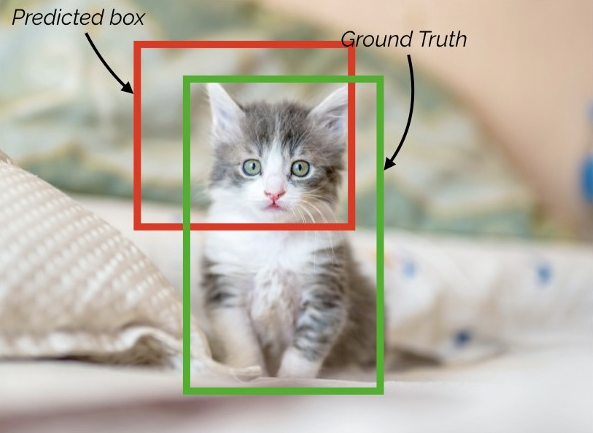
\includegraphics[width=0.9\linewidth]{obrazky-figures/iou1.png}\hfill
    \caption{IOU = 0.3, False positive}
    \end{subfigure}
    \begin{subfigure}{0.45\textwidth}
    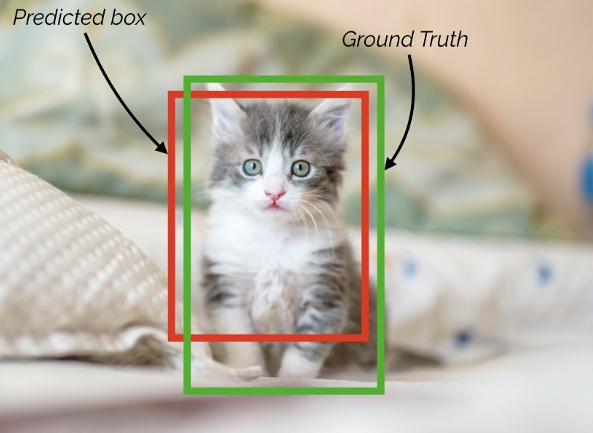
\includegraphics[width=0.9\linewidth]{obrazky-figures/iou2.png}\hfill
    \caption{IOU = 0.7, True positive}
    \end{subfigure}
    \caption{Predicted box značí detekovaný ohraničující box a ground truth předem definovaný ohraničující box. Pokud je v tomto případě IoU rovno 0.5, znamená to že obrázek a) je False positive a obrázek b) je True positive\protect\footnotemark{}.}
    \label{iou2}
\end{figure}
\footnotetext{Dostupné z \url{https://miro.medium.com/v2/resize:fit:720/format:webp/1*S8osGaPdGMnJc-WFIqR3eA.jpeg}}
\subsection*{Precision, Recall a F1 skóre}
\label{prf}

\paragraph{} Precision \cite{precision_recall} se vypočítá jako poměr mezi počtem správně klasifikovaných pozitivních vzorků a celkovým počtem vzorků klasifikovaných jako pozitivní (správně nebo nesprávně). Precision měří přesnost modelu při klasifikaci vzorku jako pozitivního. Lze vypočítat pomocí následující rovnice:

\begin{equation}
\text { P }=\frac{T P}{T P+F P}
\end{equation}

kde P je precision. Pokud model provede mnoho nesprávných pozitivních klasifikací nebo málo správných pozitivních klasifikací, zvýší se jmenovatel a přesnost se sníží. Na druhé straně je přesnost vysoká, když:
\begin{enumerate}
    \item Model provede mnoho správných pozitivních klasifikací (maximalizuje pravdivé pozitivní klasifikace).
    \item Model provede méně nesprávných pozitivních klasifikací (minimalizuje falešně pozitivní klasifikace).
\end{enumerate}


\paragraph{} Recall \cite{precision_recall} se vypočítá jako poměr mezi počtem true positives a celkovým počtem předem definovaných pozitivních vzorků, jak lze vidět v rovnici \ref{recall}. Recall měří schopnost modelu odhalit pozitivní vzorky. Čím vyšší je recall, tím více pozitivních vzorků je detekováno.

\begin{equation}\label{recall}
\text { R }=\frac{T P}{T P+F N}
\end{equation}
kde R je recall. Recall se zajímá pouze o to, zda jsou pozitivní vzorky klasifikovány správně. Pokud model klasifikuje všechny pozitivní vzorky jako pozitivní, pak bude recall 100\&, i kdyby všechny negativní vzorky byly nesprávně klasifikovány jako pozitivní.
\paragraph{} Skóre F1 \cite{precision_recall} kombinuje precision a recall následovně:

\begin{equation}
\begin{aligned}
\text { F1 } & =\frac{2}{\frac{1}{\text { P }}+\frac{1}{\text { R }}}
& =\frac{2 \times \text { P } \times \text { R }}{\text { P }+ \text { R }}
=\frac{T P}{T P+\frac{1}{2}(F P+F N)}
\end{aligned}
\end{equation}

\subsection*{Average Precision}
\label{ap}
\paragraph{}Average precision (AP) \cite{ap} je způsob, kterým lze shrnout precision-recall křivku do jediné hodnoty, která představuje průměr všech hodnot precision.
\paragraph{} Křivka precision-recall (obrázek \ref{precision_recall}) ukazuje kompromis mezi hodnotami precision a recall pro různé prahové hodnoty. Tato křivka pomáhá vybrat nejlepší práh pro maximalizaci obou metrik.


\begin{figure}
    \centering
    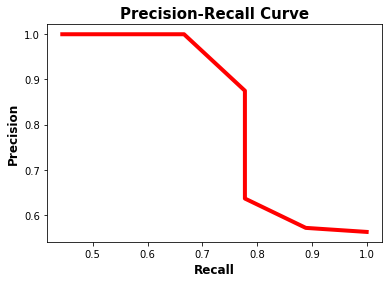
\includegraphics[width=0.5\linewidth]{obrazky-figures/precision_recall.png}
    \caption{Na obrázku lze vidět příklad křivky precision-recall.Všimněte si, že s rostoucí hodnotou recall klesá precision. Když se zvyšuje počet pozitivních vzorků (vysoký recall), klesá přesnost správné klasifikace každého vzorku (nízká precision). To je očekávatelné, protože při velkém počtu vzorků je větší pravděpodobnost, že model selže\protect\footnotemark{}.}
    \label{precision_recall}
\end{figure}
\footnotetext{Dostupné z \url{https://blog.paperspace.com/content/images/2020/09/Fig01.png}}
 \paragraph{} Average precision se vypočítá podle rovnice \ref{AP} \cite{ap}. Pomocí smyčky, která prochází všechny hodnoty precision a recall, se vypočítá rozdíl mezi aktuálním a následujícím vyvoláním a poté se vynásobí aktuální hodnotou precision. Jinými slovy, AP je vážený součet precision na každé prahové hodnotě, kde váha představuje nárůst hodnoty recall.

 \begin{equation}\label{AP}
A P=\sum n(R_n-R_{n-1}) P n
\end{equation}
Kde \begin{math}R_n\end{math} je recall v bodě prahu \textit{n} a \begin{math}P_n\end{math} je precision v bodě prahu \textit{n} na precision-recall křivce.

\subsection*{Mean Average Precision}
\paragraph{} Mean Average Precision \cite{ap} počítá Average precision napříč jednotlivými detekovanými třídami (rovnice \ref{map}). Vzhledem k tomu že v této práci detekuji pouze jednu třídu, přímo tuto metriku nevyužívám. Testované metody YOLOv5 však tuto metodu automaticky zaznamenávají. Protože se však detekuje pouze jedna třída, je tato hodnota stejná jako Average precision.

\begin{equation}\label{map}
m A P=\frac{1}{n} \sum_{k=1}^{k=n} A P_k
\end{equation}

Kde \begin{math}AP_k\end{math} je Average precision třídy \textit{k} a \textit{n} je celkový počet tříd.
\section*{Metriky trénování neuronových sítí}
\paragraph{} Některé metriky se používají pouze při trénování umělých neuronových sítí. Nazývají se ztrátové funkce. Tyto funkce měří rozdíl mezi předpovězeným výstupem modelu a předem definovanými trénovacími daty. Cílem strojového učení je minimalizovat tyto ztrátové funkce, což znamená zmenšovat rozdíly mezi předem definovanými trénovacími daty a výstupem sítě.
\paragraph{} Existuje mnoho druhů těchto funkcí, přičemž v této práci sleduju tři ztrátové funkce neuronové sítě YOLOv5. Konkrétně to jsou Classes loss, Objectness loss a Location loss\cite{ultralytics}.

\subsection*{Classes loss a Objectness loss}
\label{cls_obj_loss}
\paragraph{} Obě tyto tyto ztrátové funkce využívají ke svému výpočtu Binary cross-entropy funkci. Classes loss, nebo také classification loss, indikuje jak dobře detektor předpoví třídu detekovaného objektu. Jelikož však v této práci detekujeme pouze jeden objekt, je tato metrika vždy nula. Objectness měří pravděpodobnost, že objekt existuje v navrhované zájmové oblasti. Je-li objectness vysoká, znamená to, že detekované okno pravděpodobně obsahuje hledaný objekt \cite{loss}. Objectness loss měří rozdíl mezi objectness detekovaného ohraničující boxu a předem definovaného ohraničující boxu. Počítá se pomocí rovnice:
\begin{equation}
    1 - \delta\textit{objectness}
\end{equation}
kde \begin{math}\delta\textit{objectness}\end{math} je rozdíl mezi dvěma ohraničujícími boxy.
\paragraph{} Binary cross-entropy porovnává dvě rozdělení pravděpodobnosti ve stejné základní množině. Ztrátová funkce Binary cross-entropy pro jednu třídu je definována následovně:

 \begin{equation}
\mathcal{C}(p, t)=t \mathcal{C}_r(p)+(1-t) \mathcal{C}_l(p)
\end{equation}
kde $t \in T$, přičemž $T=\{0,1\}$ je předem definovaný štítek a $p \in P$, kde $P=(0,1)$ je výstupem detektoru a kde \begin{math}C_l(p)=-\log (1-p) \text { a }C_r(p)=-\log (p)\end{math} \cite{bce}.

\subsection*{Location loss}
\label{location_loss}
\paragraph{} Location loss, často také označována jako box loss, ukazuje jak dobře dokáže model lokalizovat střed objektu a jak dobře vygenerovaný ohraničující box tento objekt překrývá \cite{loss}. V neuronových sítích YOLOv5 je tato metrika založená na metrice Complete Intersection over Union loss \cite{ultralytics}.
\paragraph{} Původní Intersection over Union loss se dá formulovat následovně: 

\begin{equation}\label{s}
\mathcal{L}_{I o U}=1-I o U .
\end{equation}

Tento přístup však nedokáže rozpoznat případy, kdy se detekovaný ohraničující box a předem definovaný ohraničující box vůbec nepřekrývají. Zajímá se tedy pouze o oblast překrytí. Complete intersection over union loss \cite{ciou} bere v potaz tři parametry: oblast překrytí, vzdálenost a poměr stran. Obecně lze tuto metriku definovat touto rovnicí:

\begin{equation}
\mathcal{L}=S\left(\mathcal{B}, \mathcal{B}^{g t}\right)+D\left(\mathcal{B}, \mathcal{B}^{g t}\right)+V\left(\mathcal{B}, \mathcal{B}^{g t}\right)
\end{equation}
kde \textit{S} reprezentuje oblast překrytí, \textit{D} vzdálenost a \textit{V} poměr stran detekováného ohraničující boxu. \begin{math}\mathcal{B} \text{ a } \mathcal{B}^{g t}\end{math} reprezentují detekovaný ohraničující box a předem definovaný ohraničující box v tomto pořadí. 
\paragraph{} Oblast překrytí \textit{S} lze vypočítat pomocí rovnice \ref{s}. Vzdálenost \textit{D} se počítá jako normalizovaná vzdálenost mezi středovými body dvou ohraničujících boxů pomocí následující rovnice:

\begin{equation}
D=\frac{\rho^2\left(\boldsymbol{p} \cdot \boldsymbol{p}^{g t}\right)}{c^2}
\end{equation}
kde \begin{math}\boldsymbol{p} \text{ a } \boldsymbol{p}^{g t} \end{math} reprezentují ony středové body a \begin{math}\rho\end{math} je vzdálenost mezi těmito dvěma body. \begin{math}c\end{math} je délka diagonály ohraničující boxu, který překrývá jak detekovaný ohraničující box, tak ohraničující box předem definovaný (obrázek \ref{distance}). 

\begin{figure}[h]\centering
    \centering
    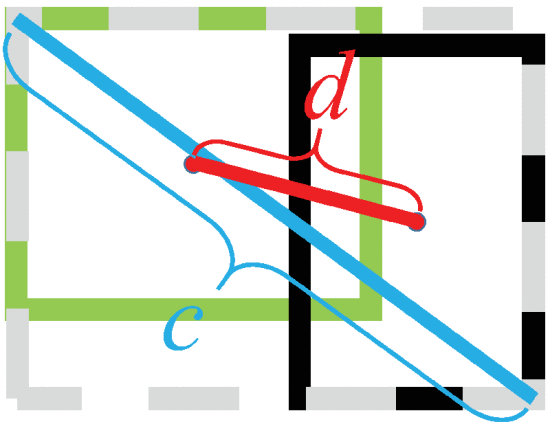
\includegraphics[width=0.6\linewidth]{obrazky-figures/distance.png}
    \caption{Na obrázku lze vidět dvojici ohraničující boxů a ohraničující box který je oba překrývá. \textit{d} je vzdálenost mezi dvěma středovými body těchto ohraničujících boxů a \textit{c} je délka diagonály překrývajícího ohraničujícího boxu\protect\footnotemark{}.}
    \label{distance}
\end{figure}
\footnotetext{Dostupné z \url{https://www.researchgate.net/publication/355101043/figure/fig4/AS:1076750272462854@1633728678747/6-DIoU-loss-for-bounding-box-regression_W640.jpg}}
\paragraph{} Poměr stran \textit{V} vypočítáme následovně:

\begin{equation}
V=\frac{4}{\pi^2}\left(\arctan \frac{w^{g t}}{h^{g t}}-\arctan \frac{w}{h}\right)^2
\end{equation}
kde \textit{w} a \textit{h} reprezentují šířku a výšku svých ohraničujících boxů. Konečně spojením těchto parametrů získáme Complete intersection over union loss:

\begin{equation}
\mathcal{L}_{\mathrm{CIoU}}=1-\mathrm{IoU}+\frac{\rho^2\left(\boldsymbol{p}, \boldsymbol{p}^{g t}\right)}{c^2}+\alpha V
\end{equation}

kde \begin{math}\alpha\end{math} je tradeoff parametr, který je definovaný následovně:

\begin{equation}
\alpha= \begin{cases}0, & \text { if } \mathrm{IoU}<0.5 \\ \frac{V}{(1-\mathrm{loU})+V}, & \text { if } \mathrm{IoU} \geq 0.5\end{cases}
\end{equation}


\section{Metody detekce založené na pravidlech}
Rozhodl jsem se evaluovat dva detektory založené na pravidlech. Prvním z nich je metoda založená na Scharrově detekci hran, která je popsána v \ref{scharr}. Druhá z těchto metod je detektor čárových kódu knihovny OpenCV, který je založený na detekci směrové koherence a je popsán v kapitole \ref{opencv}. Pro testování těchto metod jsem využil dataset popsaný v kapitole \ref{dataset}. Obě metody jsem testoval pro práhy 0.5, 0.75 a 0.9. Nejprve zde popíšu výsledky samotných metod a poté tyto výsledky porovnám.


\subsection*{Výsledky testování Scharrovy metody detekce čárových kódů}
\label{scharr_exp}
\paragraph{}Tato metoda dosáhla velmi neuspokojivých výsledků. Všechny výsledky lze vidět přehledně v tabulce \ref{scharr_table}. Při testování na celém datasetu, dosáhla tato metoda s prahem 0.5, kdy je míra detekce nejvyšší, average precision pouhé 0.0469. Čím se práh zvyšuje, tím je average precision horší. Při práhu 0.75 byla average precision rovna 0.0107 a při práhu 0.9 dokonce pouhých 0.0009. 

\paragraph{} Recall byl na úrovni prahu 0.5 roven 0.1339, což znamená, že tato metoda detekovala na prahu 0.5 13.49\% předem definovaných čárových kódů a to i přesto že detekovala větší množství čárových kódů které jimi ve skutečnosti nebyly. Při prahu 0.75 a 0.9 byl recall roven 0.0662 a 0.0056.

\paragraph{} Precision bylo při prahu 0.5 rovno 0.2577. To nám říká, že ze všech detekovaných čárových kódů, bylo 25.77\% z nich true positive. Na úrovních prahu 0.75 a 0.9 tato hodnota klesla na 0.1181 a 0.0094. Hodnota F1 byla na prahu 0.5 rovna 0.1763 a postupně se snižovala se zvyšujícím se prahem na 0.0848 a 0.007.

\paragraph{} Při samostatném testování aliasovaných s ostatních čárových kódu se ukázal propastný rozdíl mezi těmito dvěma částmi datasetu. Zatímco při testování nealiasovaných obrázků s prahem 0.5 bylo average precision rovno 0.0469, při stejném prahu měla aliasovaná sada average precision pouhé 0.0232. Což je přibližně dvojnásobné zmenšení. Toto platí také na ostatních prahových úrovních. Nealisovaná sada měla na úrovni prahu 0.75 hodnotu average precision 0.0227 a při prahu 0.9 byla average precision 0.0009. Aliasovaná sada mělá při prahu 0.75 average precision rovnu 0.0077 a při prahu 0.9 byla average precision 0.0002.

\paragraph{} Podobné rozdíly jdou vidět v jiných metrikách, kdy při prahové hodnotě 0.5 byla u nealiasované sady hodnota recall 0.1955, precision 0.2584 a F1 0.2225. U aliasované sady byl recall pouhé 0.05294, precision byl velmi podobný a to 0.2547 a F1 0.0876. Precision byl v porovnání s ostatními metrikami velmi vysoký, protože v aliasovaném obrazu tato metoda nedetekuje mnoho objektů. Při prahových hodnotách 0.75 a 0.9 je u nealisované sady recall roven 0.1052 a 0.0101, precision 0.125 a 0.01083 a F1 0.1143 a 0.0104. U aliasované sady se na těchto prahových hodnotách recall rovná 0.01829 a 0.0005, precision 0.0849 a 0.0024 a F1 0.0301 a 0.0008.

\paragraph{} Průměrným časem této metody  pro detekci ohraničující boxu byla 0.44 vteřiny.

\begin{table}[ht]
\centering
\begin{tabular}{|l|c|c|c|c|}
\hline
Práh - dataset     & Average precision & Recall  & Precision & F1      \\ \hline
0.5 - aliased & 0.0232 & \multicolumn{1}{l|}{0.0529} & \multicolumn{1}{l|}{0.2547 } & \multicolumn{1}{l|}{0.0877} \\ \hline
0.5 - not aliased  & 0.0469           & 0.1955 & 0.2583   & 0.2226 \\ \hline
0.5 - combined     & 0.0469           & 0.1339 & 0.2577    & 0.1763\\ \hline
0.75 - aliased     & 0.0077             & 0.0183  & 0.0849    & 0.0301  \\ \hline
0.75 - not aliased &  0.0227            & 0.1052 & 0.125   & 0.1143 \\ \hline
0.75 - combined    & 0.0107            & 0.0662 & 0.1181   & 0.0848  \\ \hline
0.9 - aliased      & 0.0002               & 0.0005     & 0.0024       & 0.0008     \\ \hline
0.9 - not aliased  & 0.0009               & 0.0101     & 0.0108       & 0.0104     \\ \hline
0.9 - combined     & 0.0008               & 0.0056     & 0.0094       & 0.007     \\ \hline
\end{tabular}
\caption{V této tabulce jsou přehledně zapsány naměřené metriky Scharrovy metody detekce čárových kódů.}
\label{scharr_table}
\end{table}


\subsection*{Výsledky testování detektoru čárových kódů knihovny OpenCV}
\label{opencv_exp}
\paragraph{} Metoda detektoru čárových kódů knihovny OpenCV dosáhla na úrovni prahu 0.5 lepších výsledků. Všechny výsledky jdou vidět přehledně v tabulce \ref{opencv_table}. Na celé testovací sadě bylo average precision 0.3128, recall 0.3818, precision 0.8603 a skóre F1 0.5289. S rostoucí hodnotou prahu se však schopnost detekce rapidně snižuje. Při prahu 0.75 bylo average precision pouhé 0.03931, recall 0.1344, precision 0.2162 a F1 0.1657. Při prahu 0.9 se této metodě nepodařilo detekovat nic, všechny metriky jsou tedy 0. Je však nutno podotknout, že tato metoda má v sobě zabudované i dekódovnání čárových kódů. Je-li tedy konečným cílem detekce čárových kódů jejich dekódování, je tato metrika také relevantní. Při samotné detekci se této metodě podařilo dekódovat 41.79\% čárových kódů.
\paragraph{} Lze tady opět vidět velký rozdíl mezi aliasovanou sadou a nealiasovanou sadou. Při prahu 0.5 má nealiasovaná sada average precision 0.5037, recall 0.5004, precision 0.9234 a skóre F1 0.649. Naproti tomu aliasovaná sada při stejné prahové hodnotě average precision rovnu pouhých 0.1114, recall 0.1591, precision 0.6128 a skóre F1 0.2526. 
\paragraph{} Při stoupajících prahových hodnotách metriky v obou případech strmě klesají. U nealiasovaných obrázků při prahové hodnotě 0.75 je average precision 0.0692, recall 0.2158, precision 0.2537 a F1 0.2332. U aliasovaých obrázků při stejné prahové hodnotě je average precision 0.0063, recall 0.0209, precision 0.0693 a F1 0.03215. Při prahové hodnotě 0.9 u aliasované i nealiasované sady, stejně jako u celé datové sady, není detekován žádný čárový kód. Metriky jsou tedy nulové.
\paragraph{} U dekódování čárových kódů je rozdíl mezi aliasovanou a nealisovanou sadou také znatelný. Při detekci na nealiasované sadě se podařilo dekódovat 52.02\% čárových kódů. U aliasované sady to bylo 23.59\%. Rychlost detekce je přibližně 0.29 sekundy na čárový kód a to i s načítáním a přípravou vstupních dat.

\begin{table}[ht]
\centering
\begin{tabular}{|l|c|c|c|c|}
\hline
Práh - dataset     & Average precision & Recall  & Precision & F1      \\ \hline
0.5 - aliased & 0.1114 & \multicolumn{1}{l|}{0.1591} & \multicolumn{1}{l|}{0.6128} & \multicolumn{1}{l|}{0.2526} \\ \hline
0.5 - not aliased  & 0.5037           & 0.5004 & 0.9234   & 0.639 \\ \hline
0.5 - combined     & 0.3128           & 0.3818 & 0.8603    & 0.5289 \\ \hline
0.75 - aliased     & 0.0063             & 0.0209  & 0.0692    & 0.0322  \\ \hline
0.75 - not aliased & 0.0692            & 0.2158 & 0.2537   & 0.2332 \\ \hline
0.75 - combined    & 0.0393            & 0.1344 & 0.2162   & 0.1657  \\ \hline
0.9 - aliased      & 0               & 0     & 0       & 0     \\ \hline
0.9 - not aliased  & 0               & 0     & 0       & 0     \\ \hline
0.9 - combined     & 0               & 0     & 0       & 0     \\ \hline
\end{tabular}
\caption{V této tabulce jsou přehledně zapsány naměřené metriky detektoru čárových kódů knihovny OpenCV.}
\label{opencv_table}
\end{table}

\subsection*{Zhodnocení} Na úrovni prahu 0.5 a 0.75 je detektor čárových kódů knihovny OpenCV lepší než detektor založený na metode Scharrovy detekce ve všech metrikách. Je zároveň 1.5x rychlejší. Také umí čárové kódy sám dekódovat. Selhává sice na úrovni prahu 0.9, ale zvládá dekódovat čárové kódy i s daleko nižší kvalitou detekce čárového kódu.

\begin{figure}[h]\centering
    \centering
    \begin{subfigure}{0.9\textwidth}
    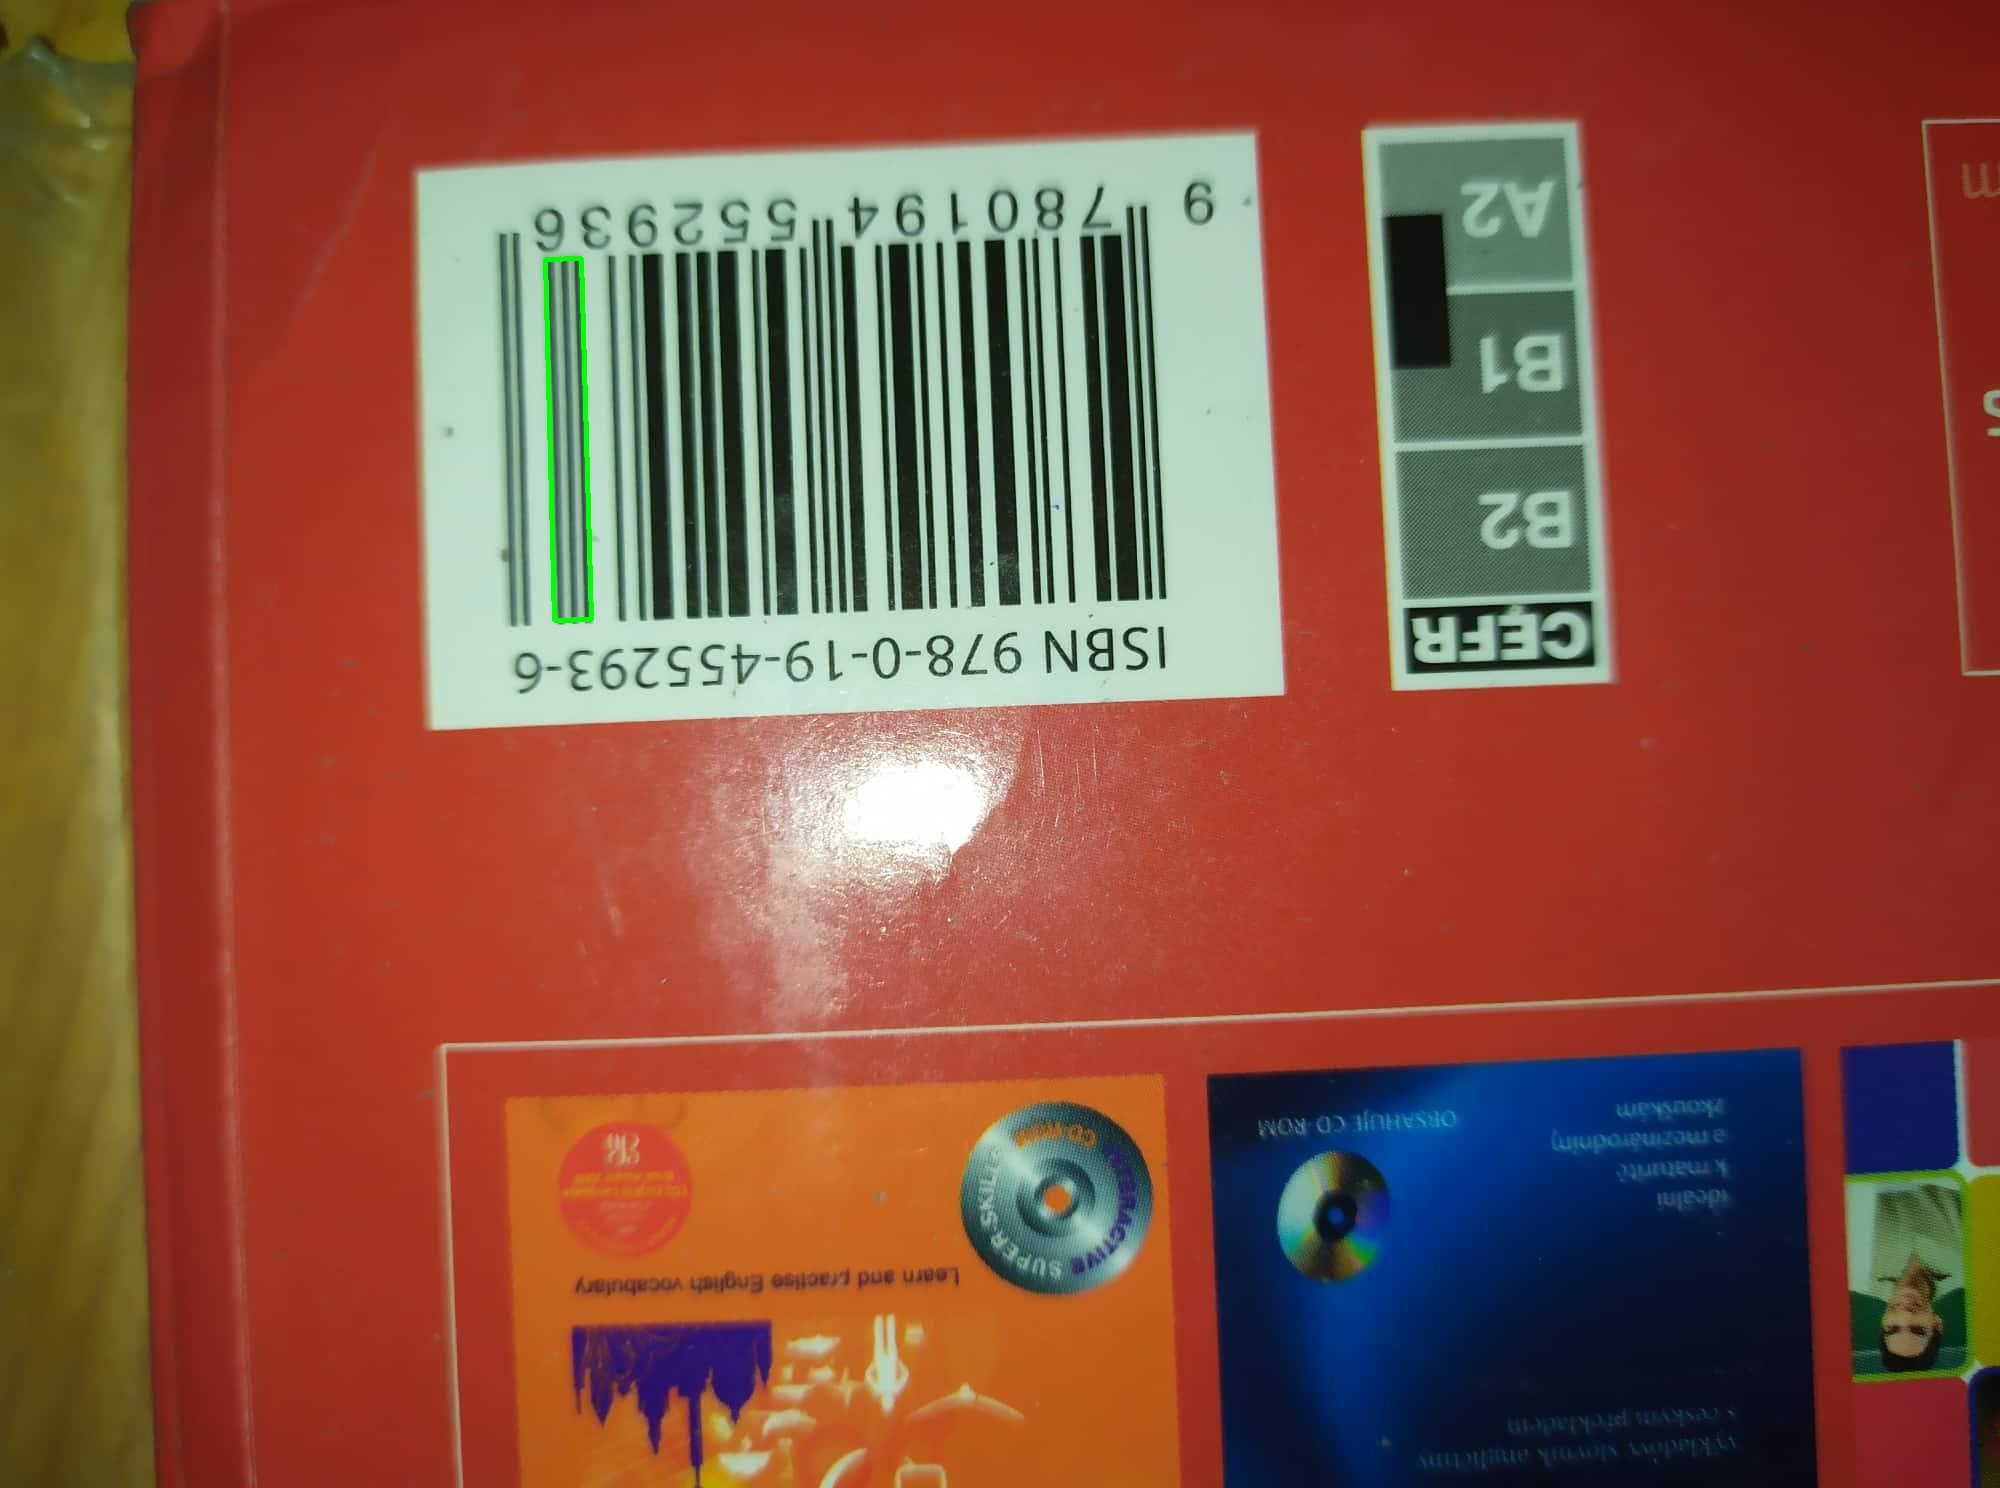
\includegraphics[width=0.4\linewidth]{obrazky-figures/scharr_test1.jpg}\hfill
    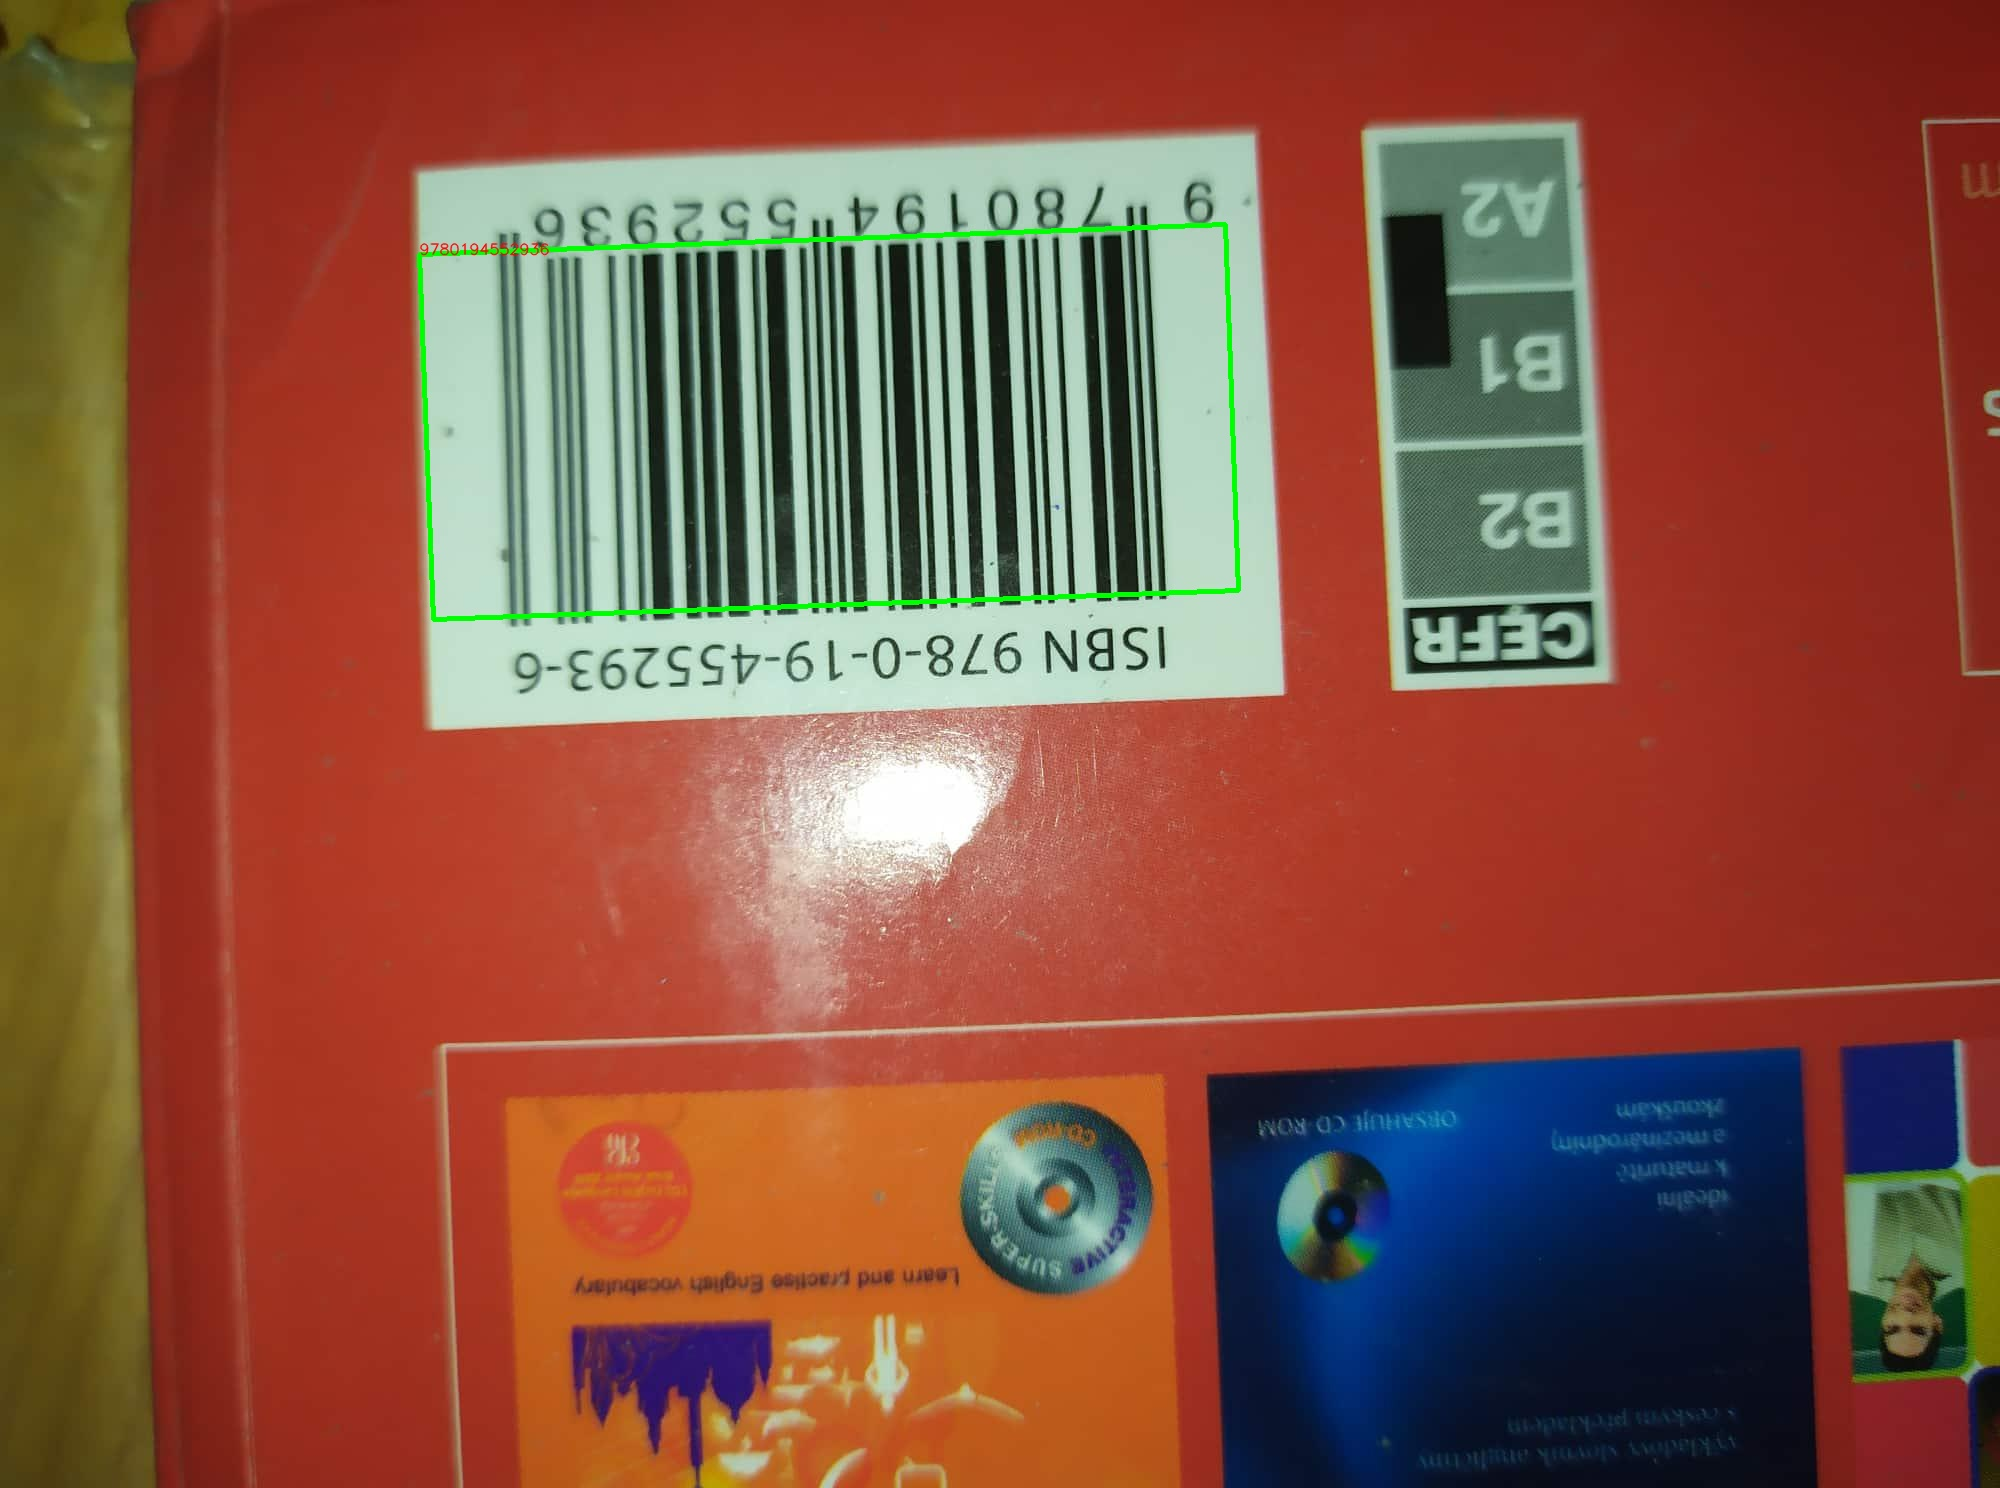
\includegraphics[width=0.4\linewidth]{obrazky-figures/opencv_test1.jpg}\hfill
    \caption{Aliasované obrázky}
    \end{subfigure}
    \begin{subfigure}{0.9\textwidth}
    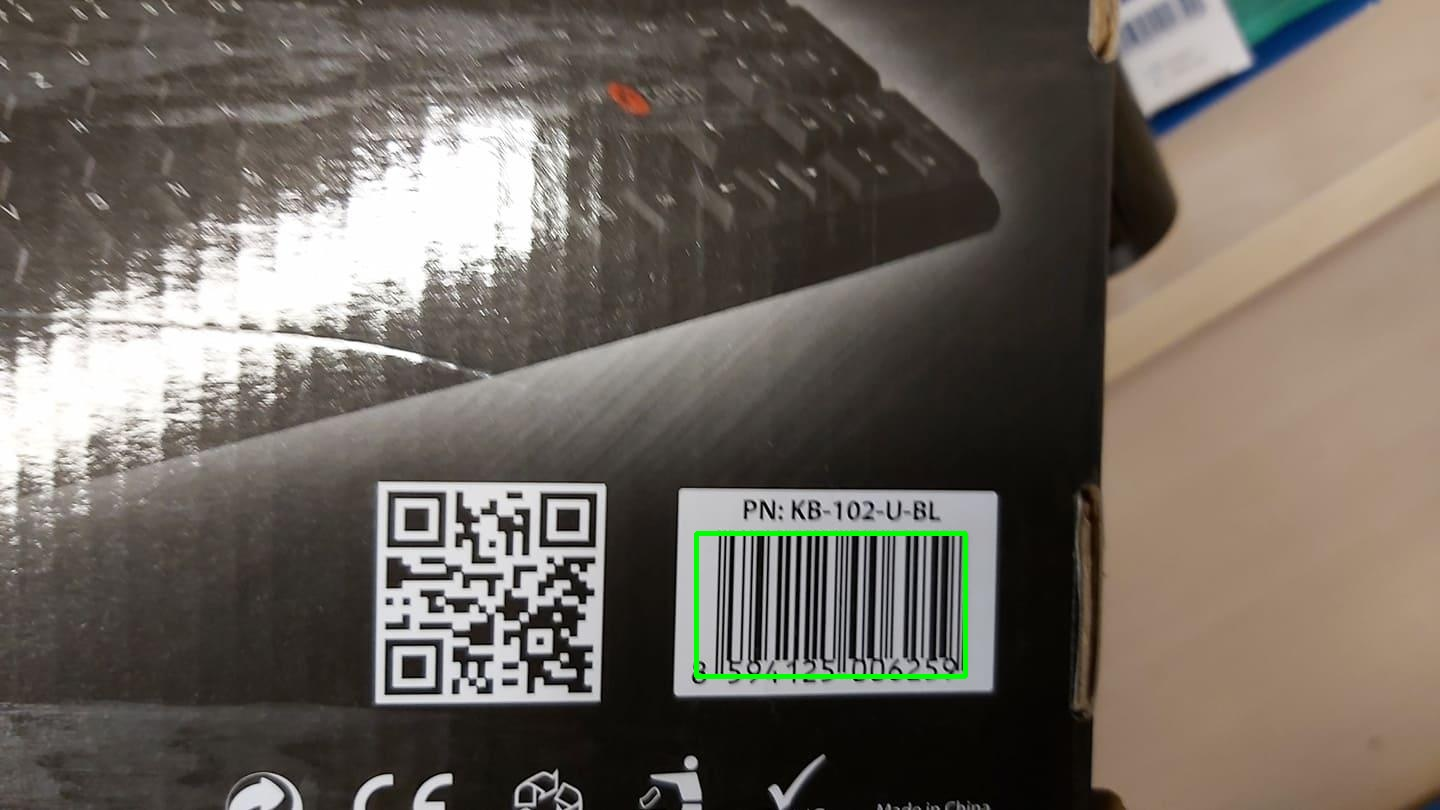
\includegraphics[width=0.4\linewidth]{obrazky-figures/scharr_test3.jpg}\hfill
    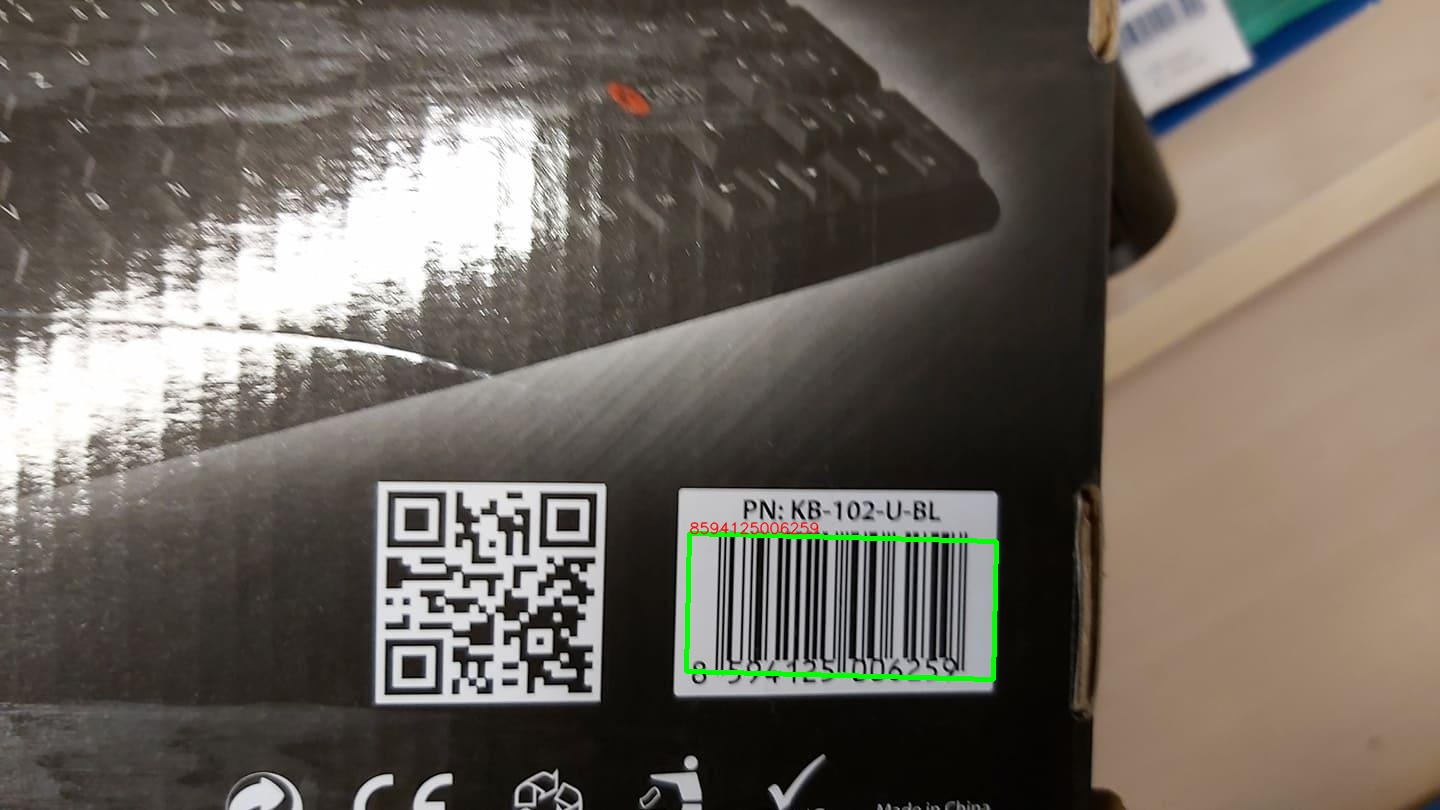
\includegraphics[width=0.4\linewidth]{obrazky-figures/opencv_test3.jpg}\hfill
    \caption{Nealiasované obrázky}
    \end{subfigure}
    \begin{subfigure}{0.9\textwidth}
    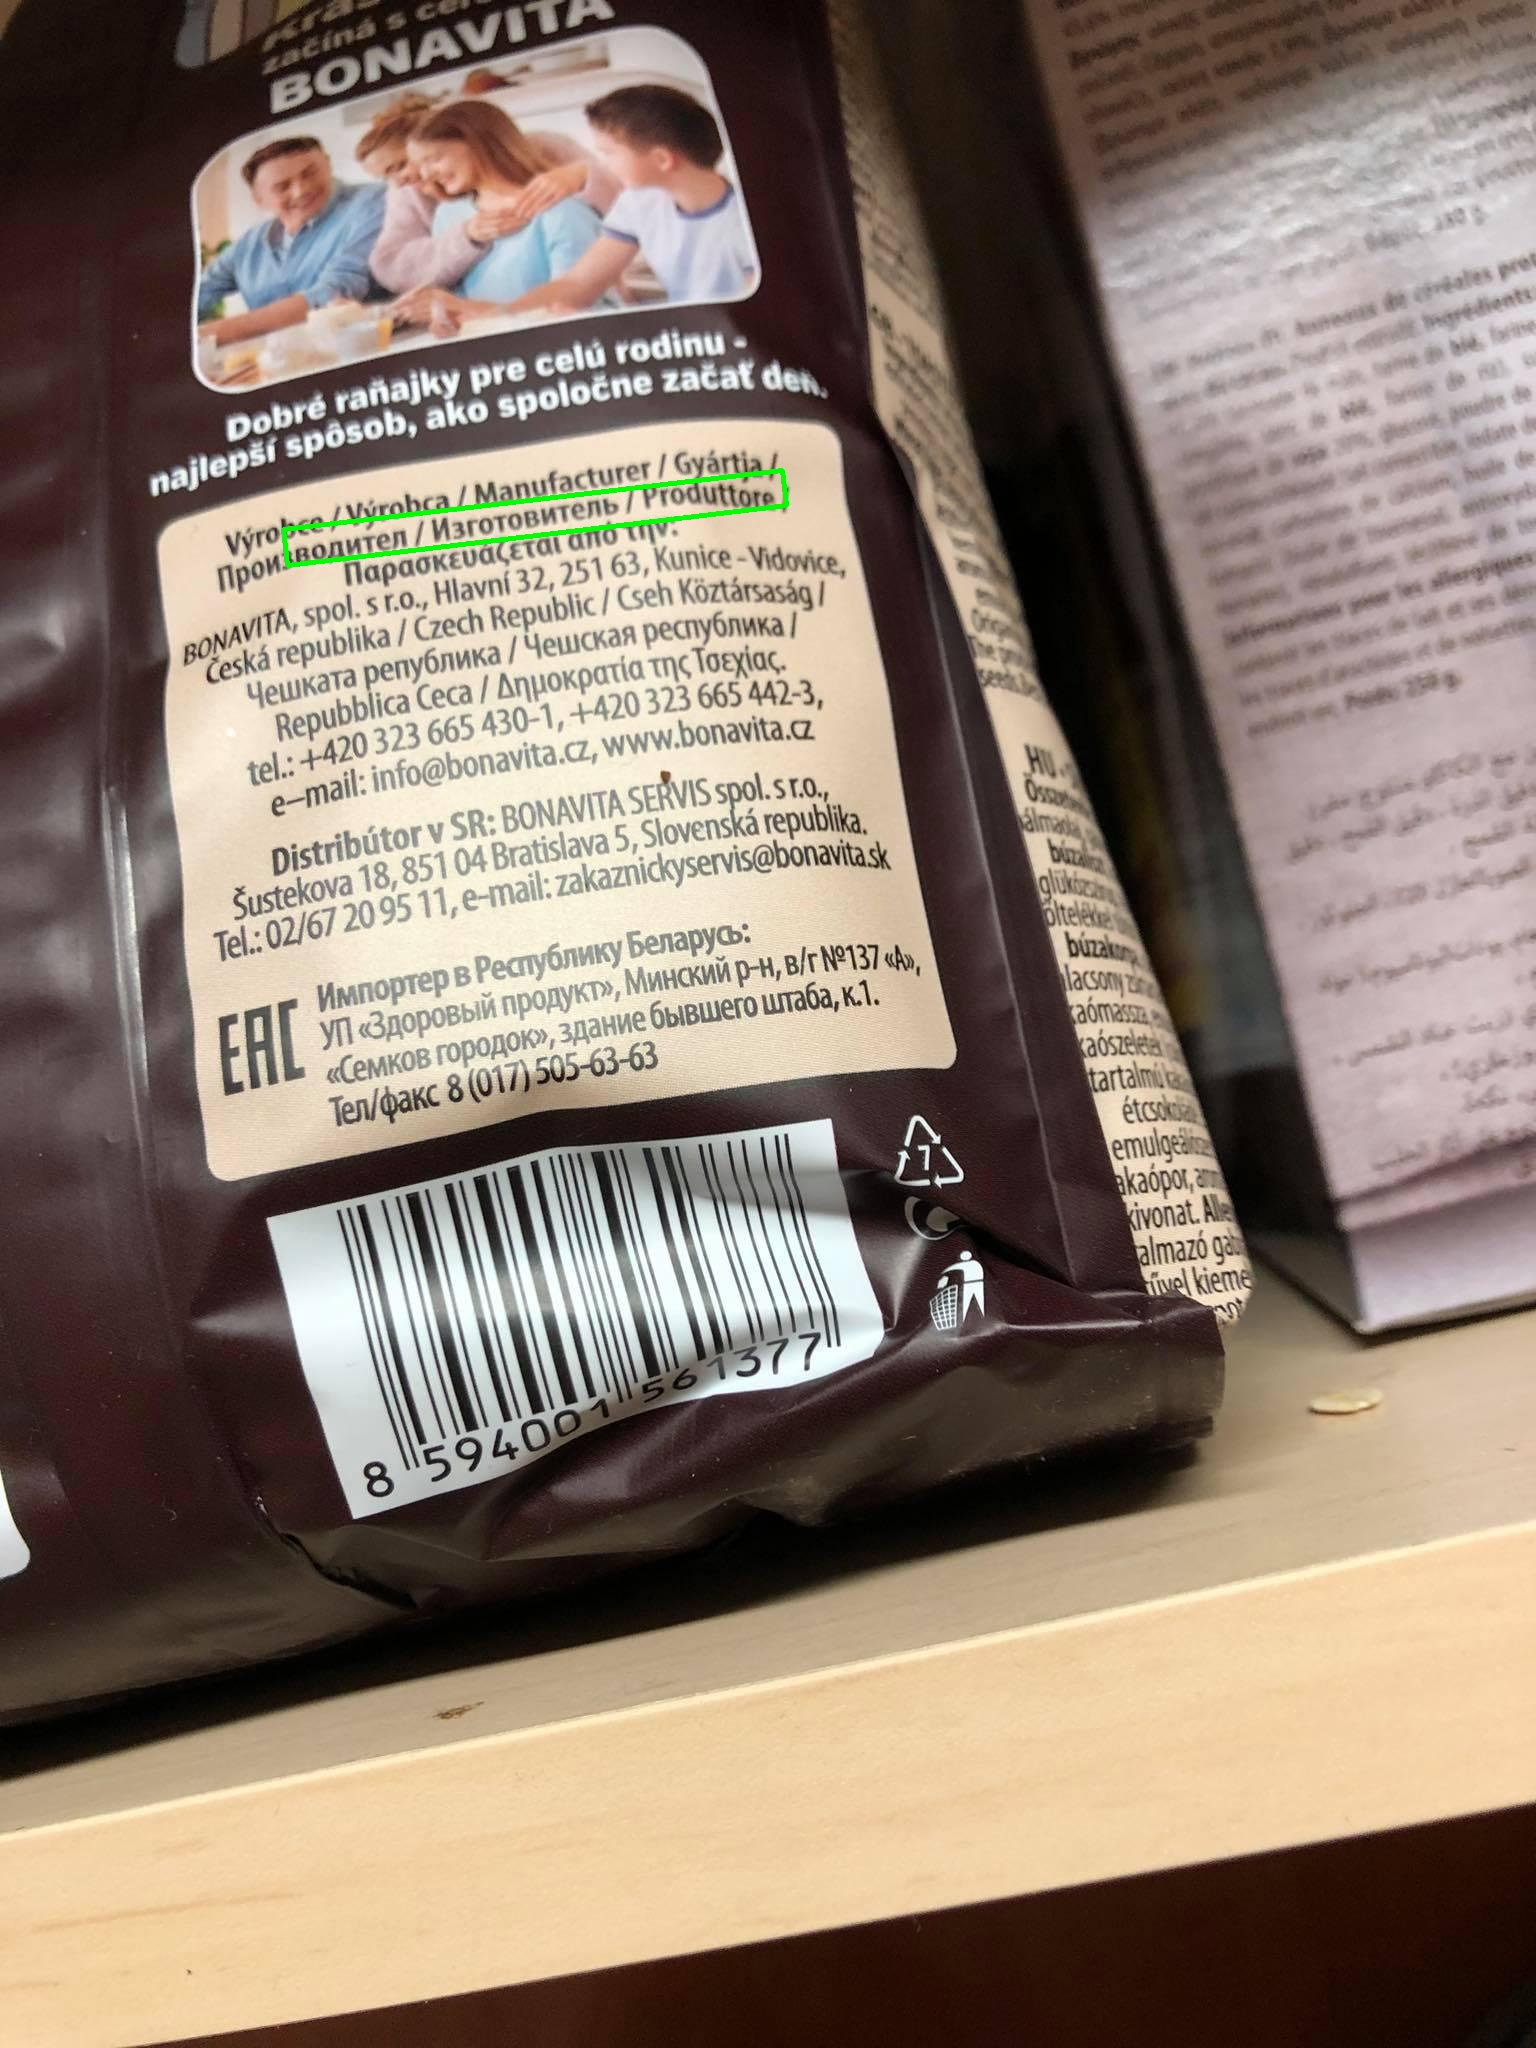
\includegraphics[width=0.4\linewidth]{obrazky-figures/scharr_test4.jpg}\hfill
    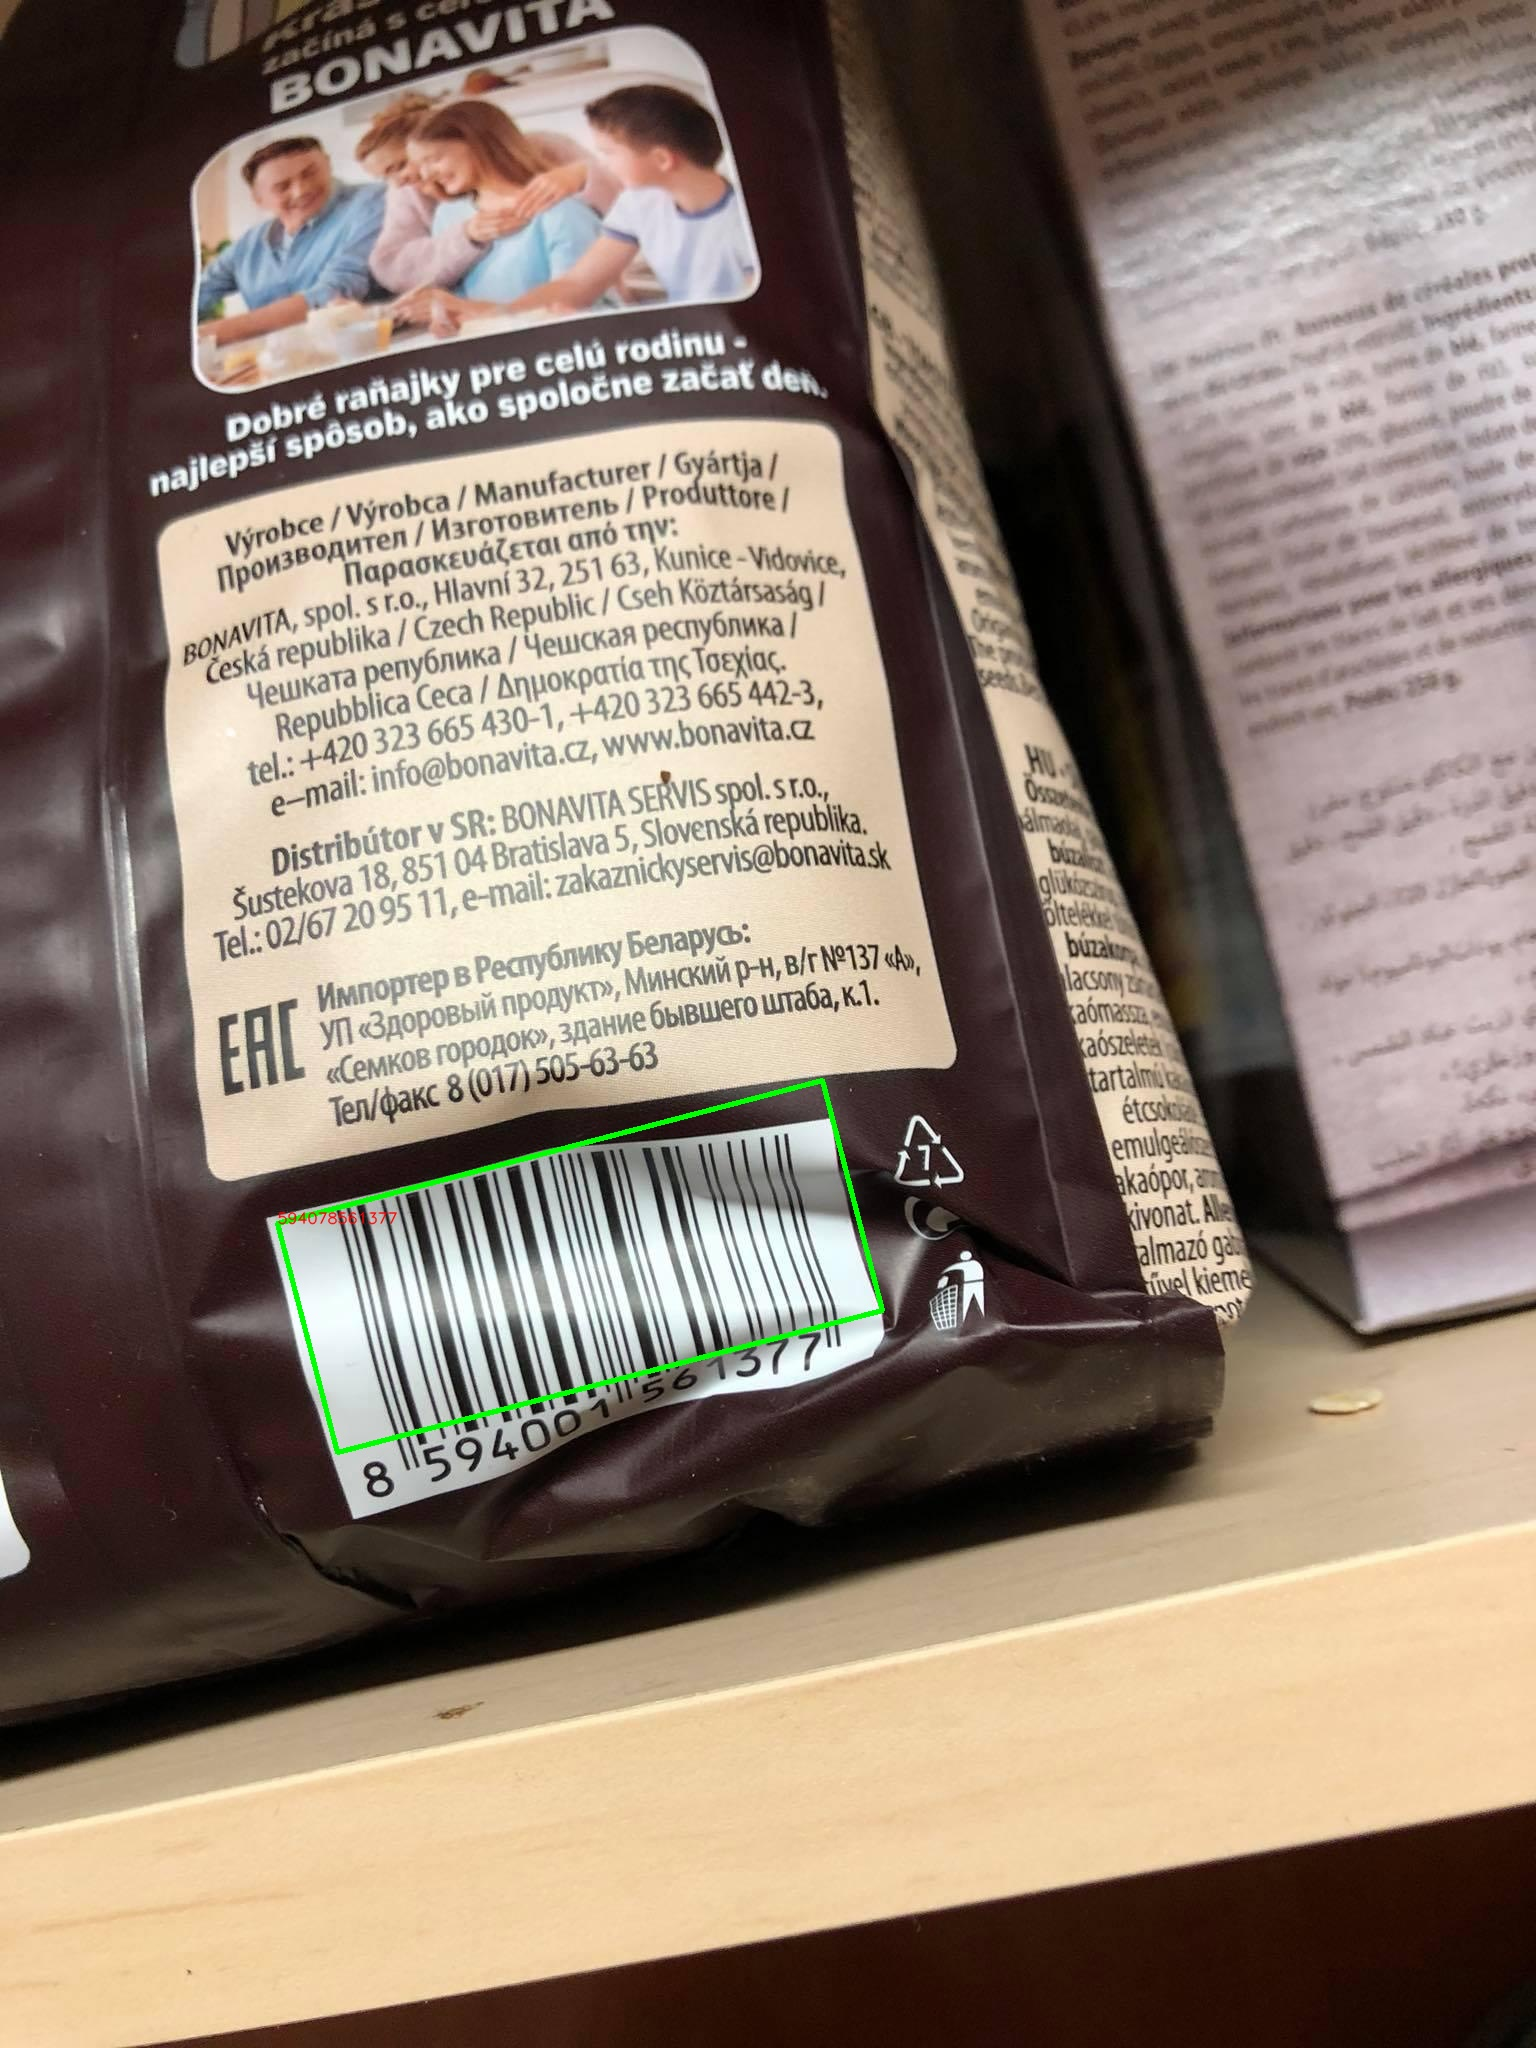
\includegraphics[width=0.4\linewidth]{obrazky-figures/opencv_test4.jpg}\hfill
    \caption{Nealiasované obrázky}
    \end{subfigure}
    \caption{Příklady detekce Scharrovy metody detekce (vlevo) a detektoru čárových kódů knihovny OpenCV (vpravo). První pár obrázků je aliasovaný, zbylé dva nejsou. Malý červený nápis u obrázků detekovaných detektorem knihovny OpenCV, představuje dekódovaný čárový kód.}
    \label{iou}
\end{figure}

\clearpage
\section{Metody detekce používající neuronové sítě}
\paragraph{} V této sekci budu evaluovat neuronovou síť YOLOv5. Pro testování této sítě jsem použil dataset popsaný v sekci \ref{dataset}. Síť YOLOv5 byla trénována na neorientované sadě, tedy sadě kde štítky představovali čtverce nebo obdélníky, které tato síť detekuje. Použil jsem předtrénovaný model yolov5s, což je druhý nejmenší a druhý nejrychlejší model sítě YOLOv5. Následný trénink sítě trval čtyřista epoch.
\subsection*{Umělá neuronová síť YOLOv5}
\label{yolov5_exp}
\paragraph{} Při práci s neorientovaným datasetem dosáhla tato metoda dobrých výsledků. Při tréninku dosáhl location loss (box loss) ve finální epoše hodnotu 0.0132 a při validaci 0.0129 jak lze vidět v grafech \ref{box1}. Čím menší je tato hodnota, tím menší je průměrný rozdíl mezi detekovaným a předem definovaným ohraničující boxem. 

\begin{figure}[h]\centering
    \centering
    \begin{subfigure}{0.7\textwidth}
    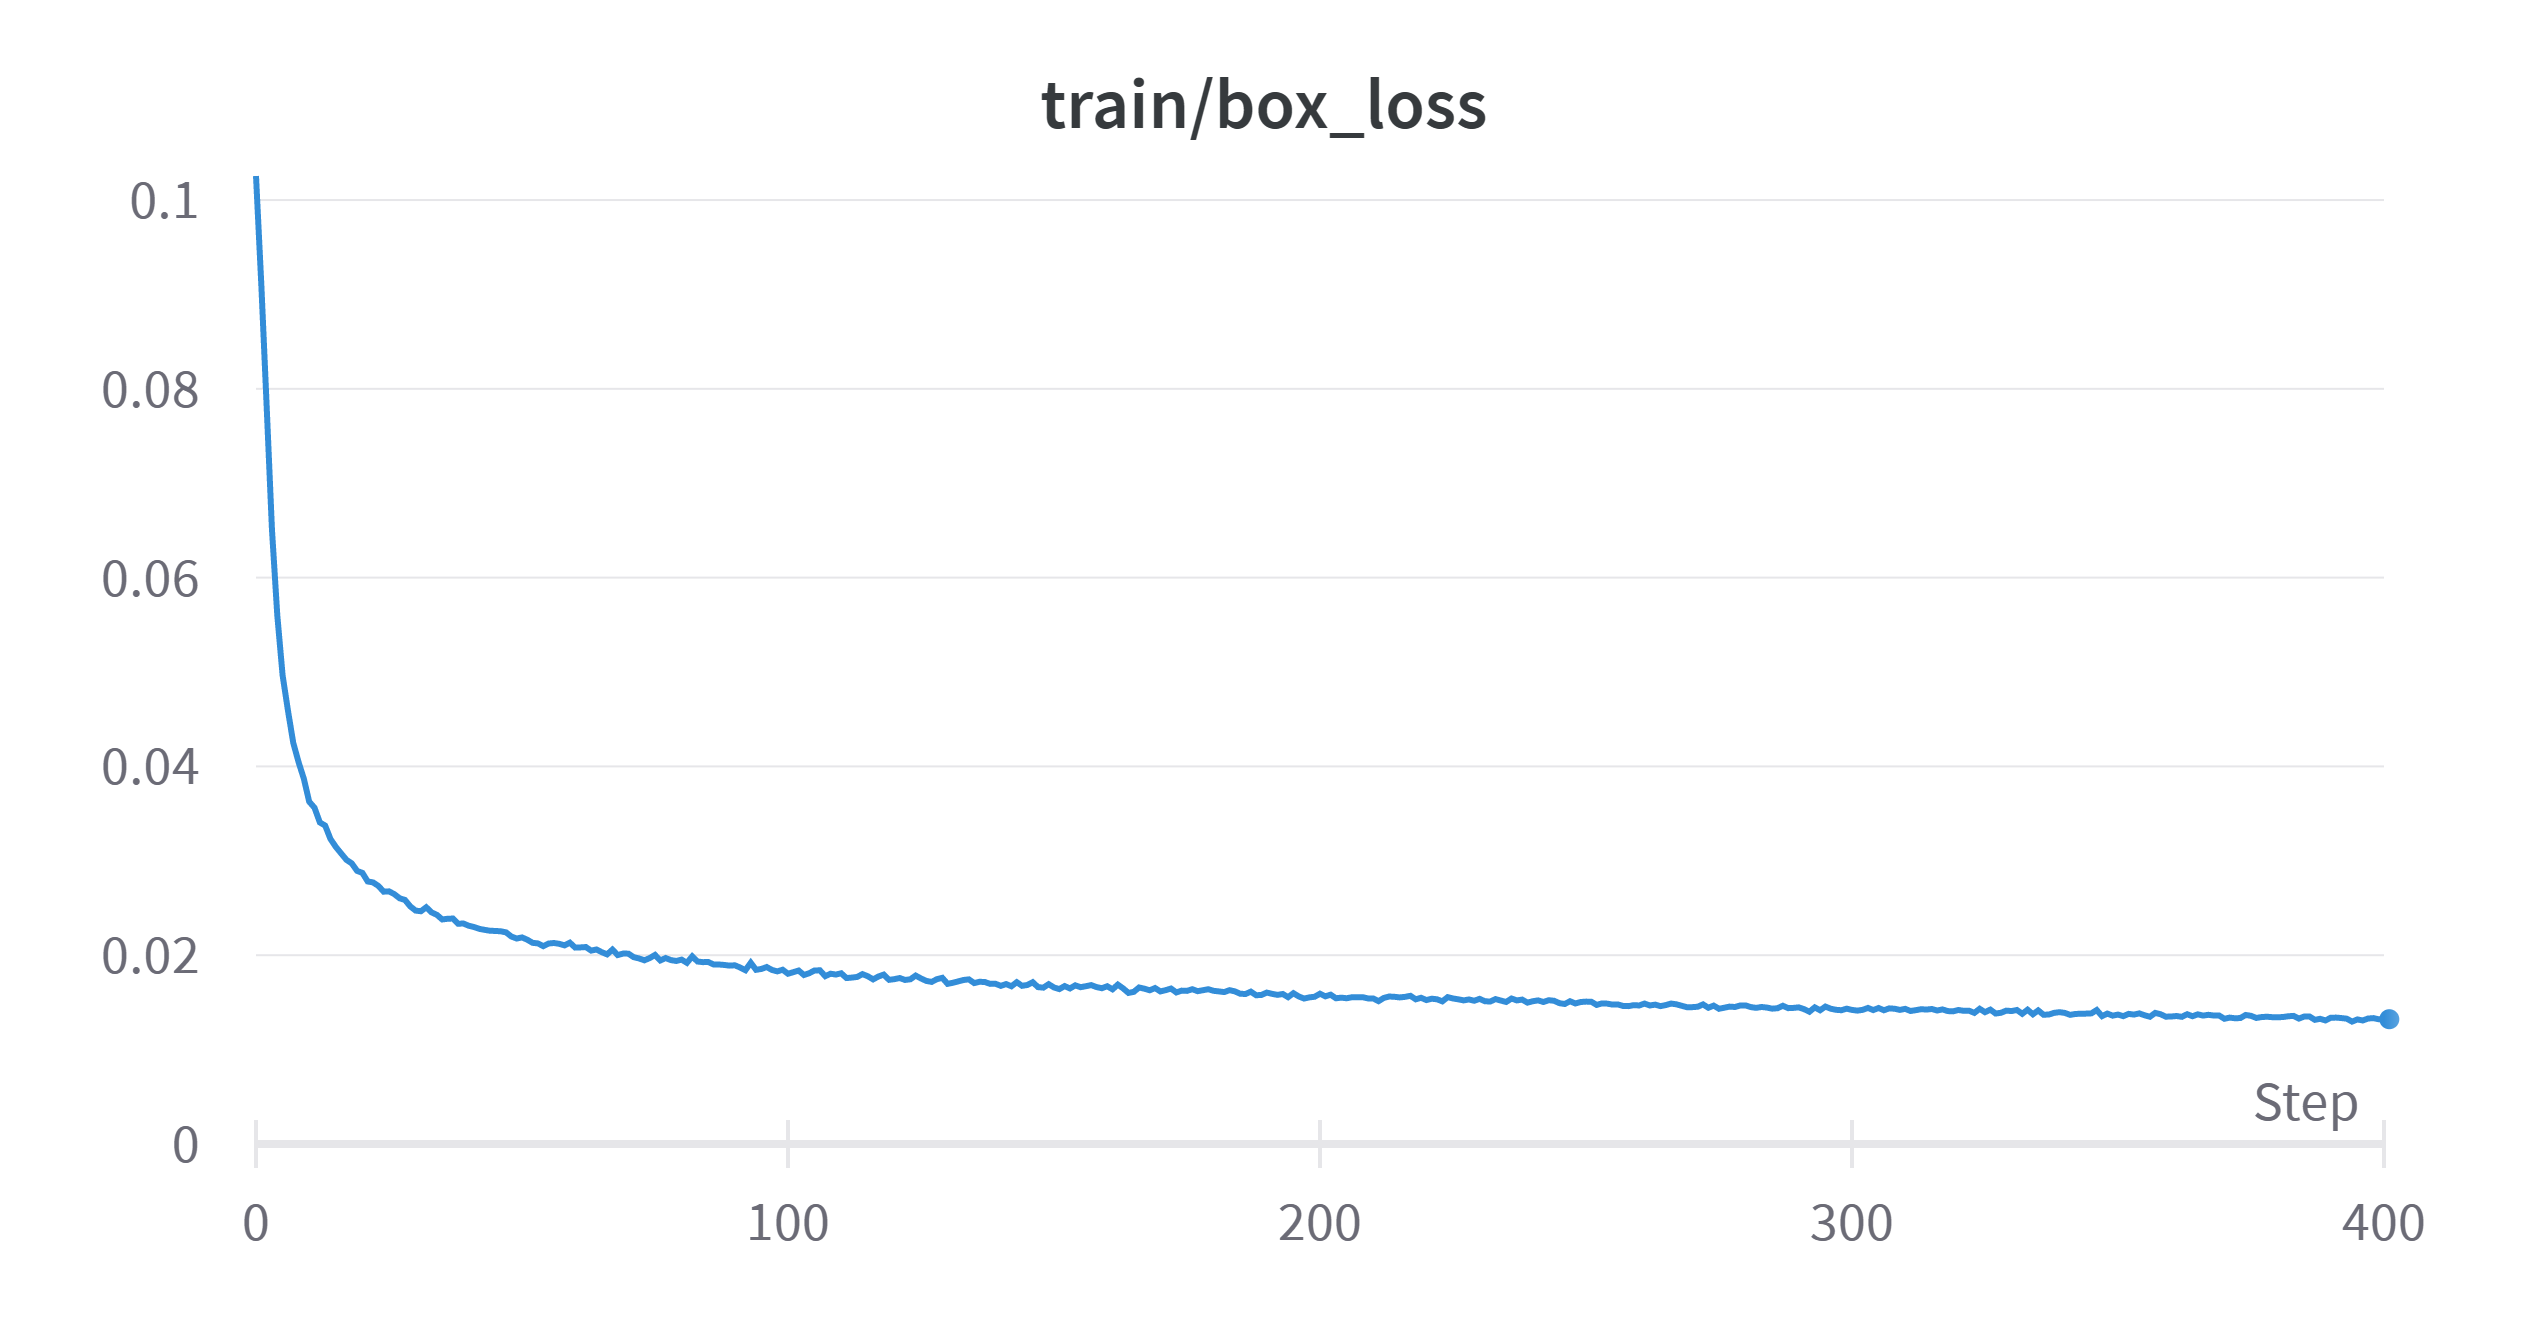
\includegraphics[width=0.95\linewidth]{obrazky-figures/train_box1.png}\hfill
    \caption{Location loss při tréninku}
    \end{subfigure}
    \begin{subfigure}{0.7\textwidth}
    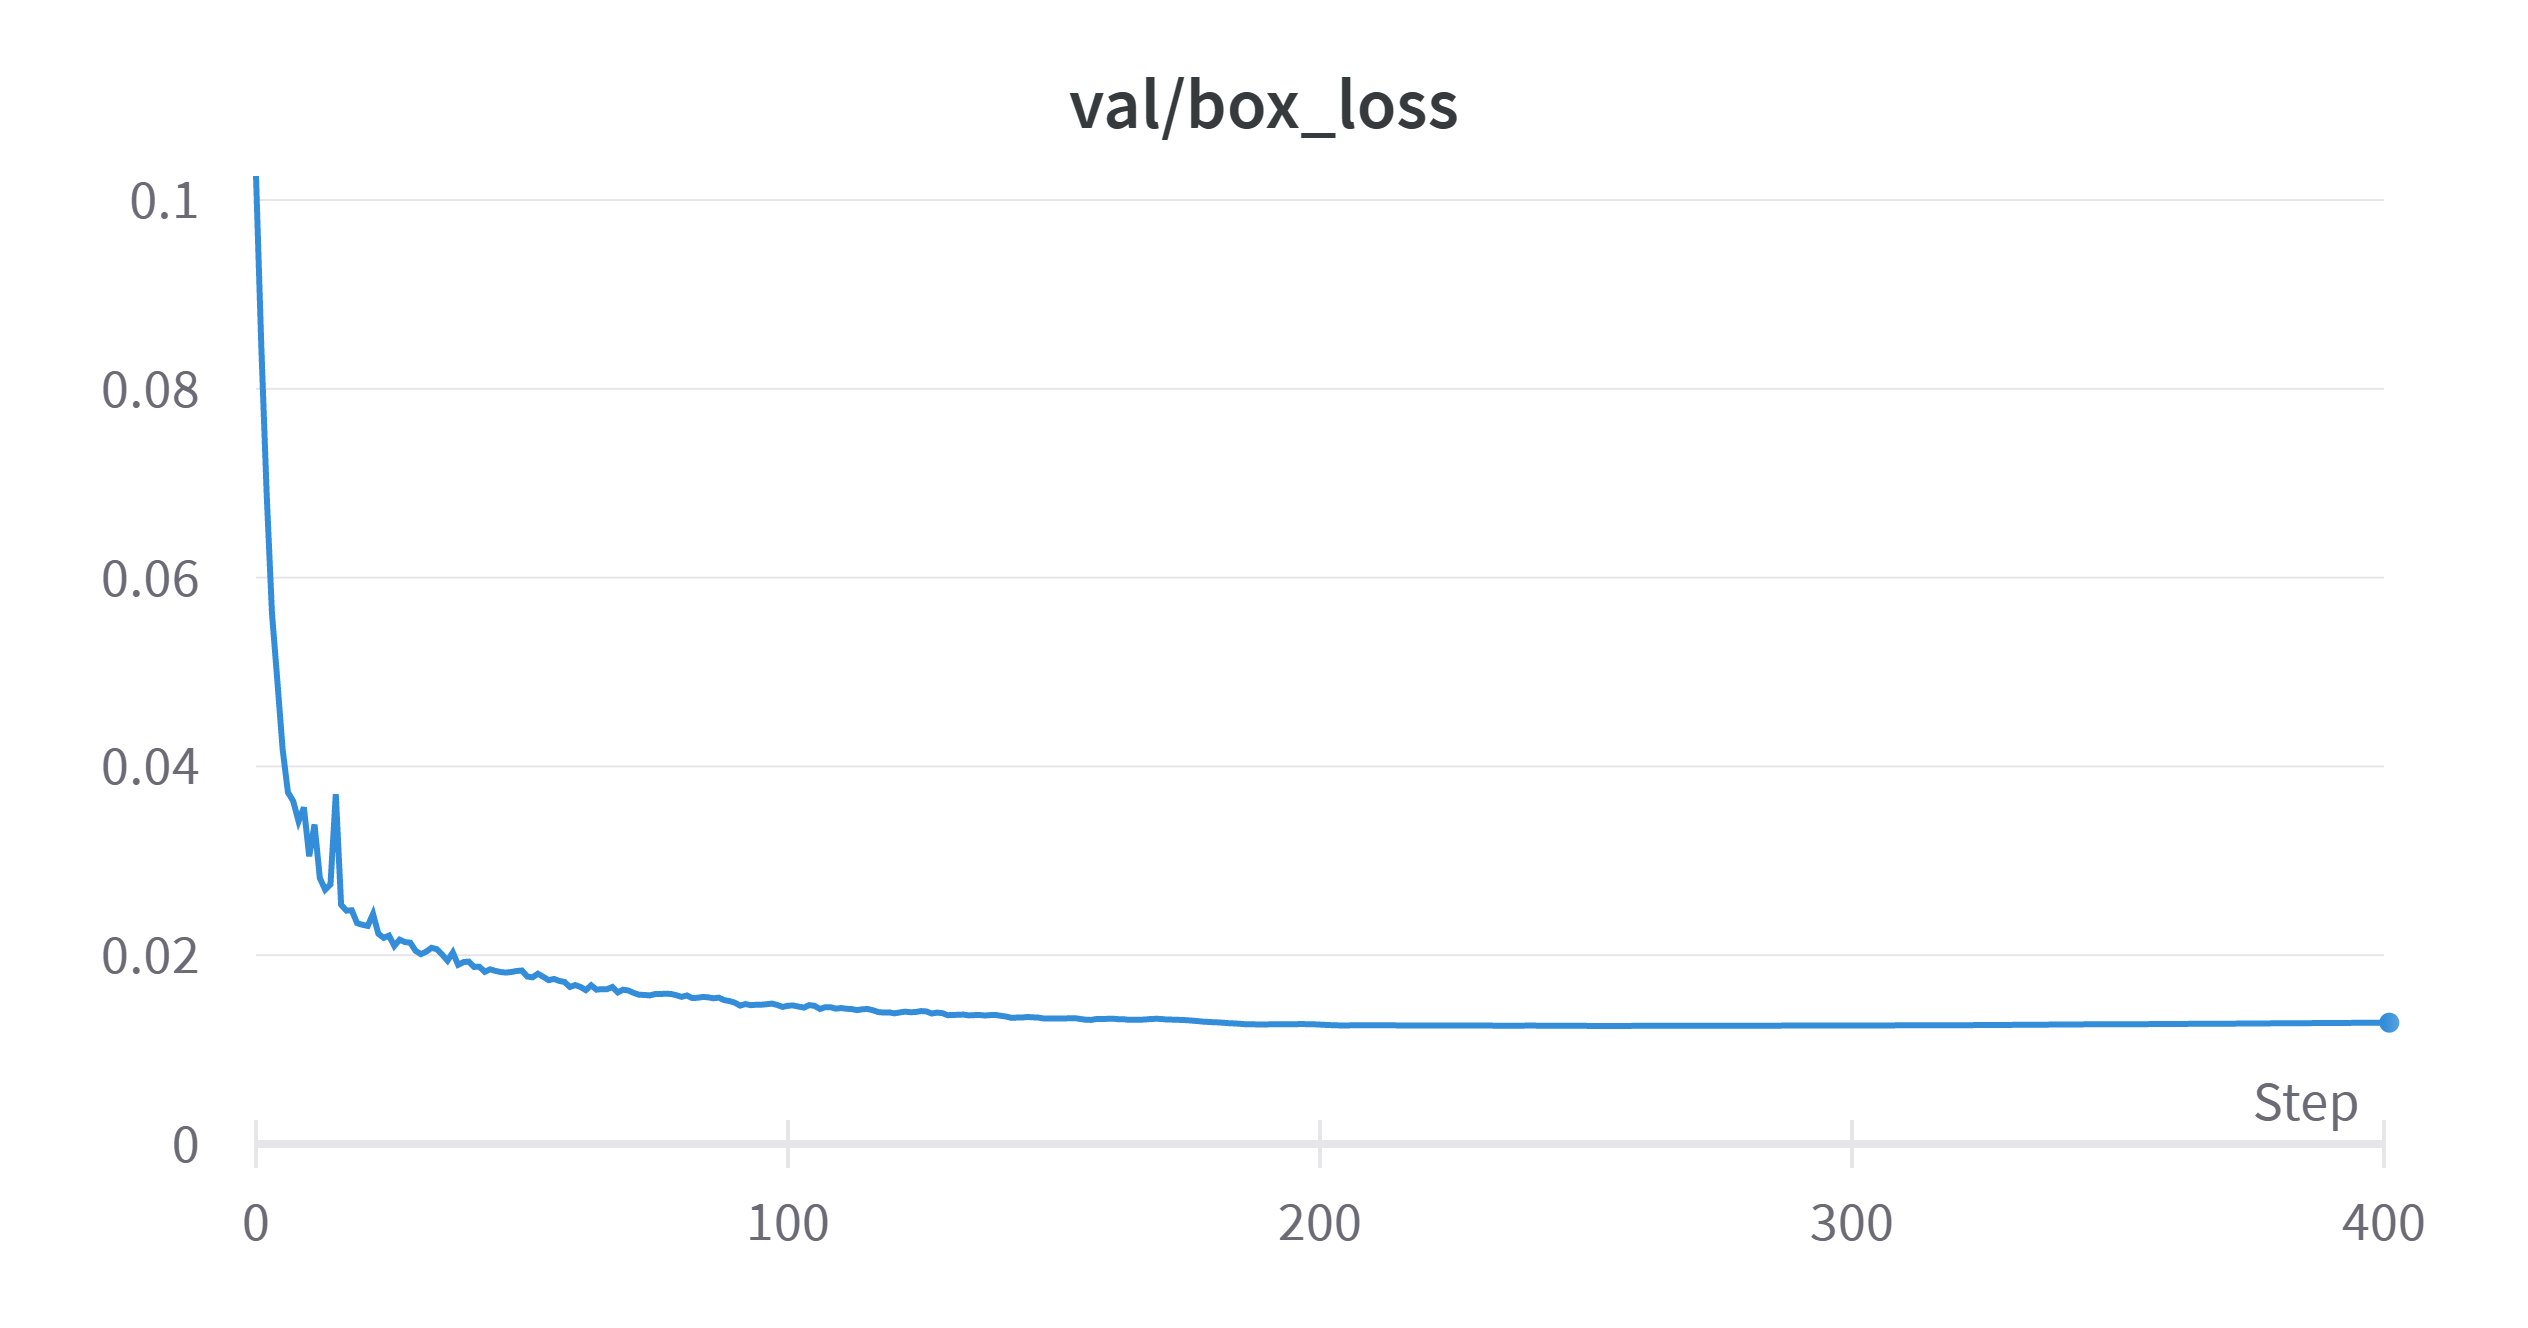
\includegraphics[width=0.95\linewidth]{obrazky-figures/box_val1.png}\hfill
    \caption{Location loss při validaci}
    \end{subfigure}
    \caption{Location loss sítě YOLOv5 v jednotlivých epochách. Čím menší je hodnota, tím menší jsou rozdíly mezi ohraničující boxy. Z grafů lze vidět jak se tato metrika s průběhem epoch zlepšuje. Validační graf má větší rozptyl hodnot, zejména kvůli menšímu množství dat. }
    \label{box1}
\end{figure}

Objectness loss byla při tréninku v konečné epoše 0.0054 a při validaci 0.0048 jak lze vidět na grafech \ref{obj1}. 

\begin{figure}[h]\centering
    \centering
    \begin{subfigure}{0.7\textwidth}
    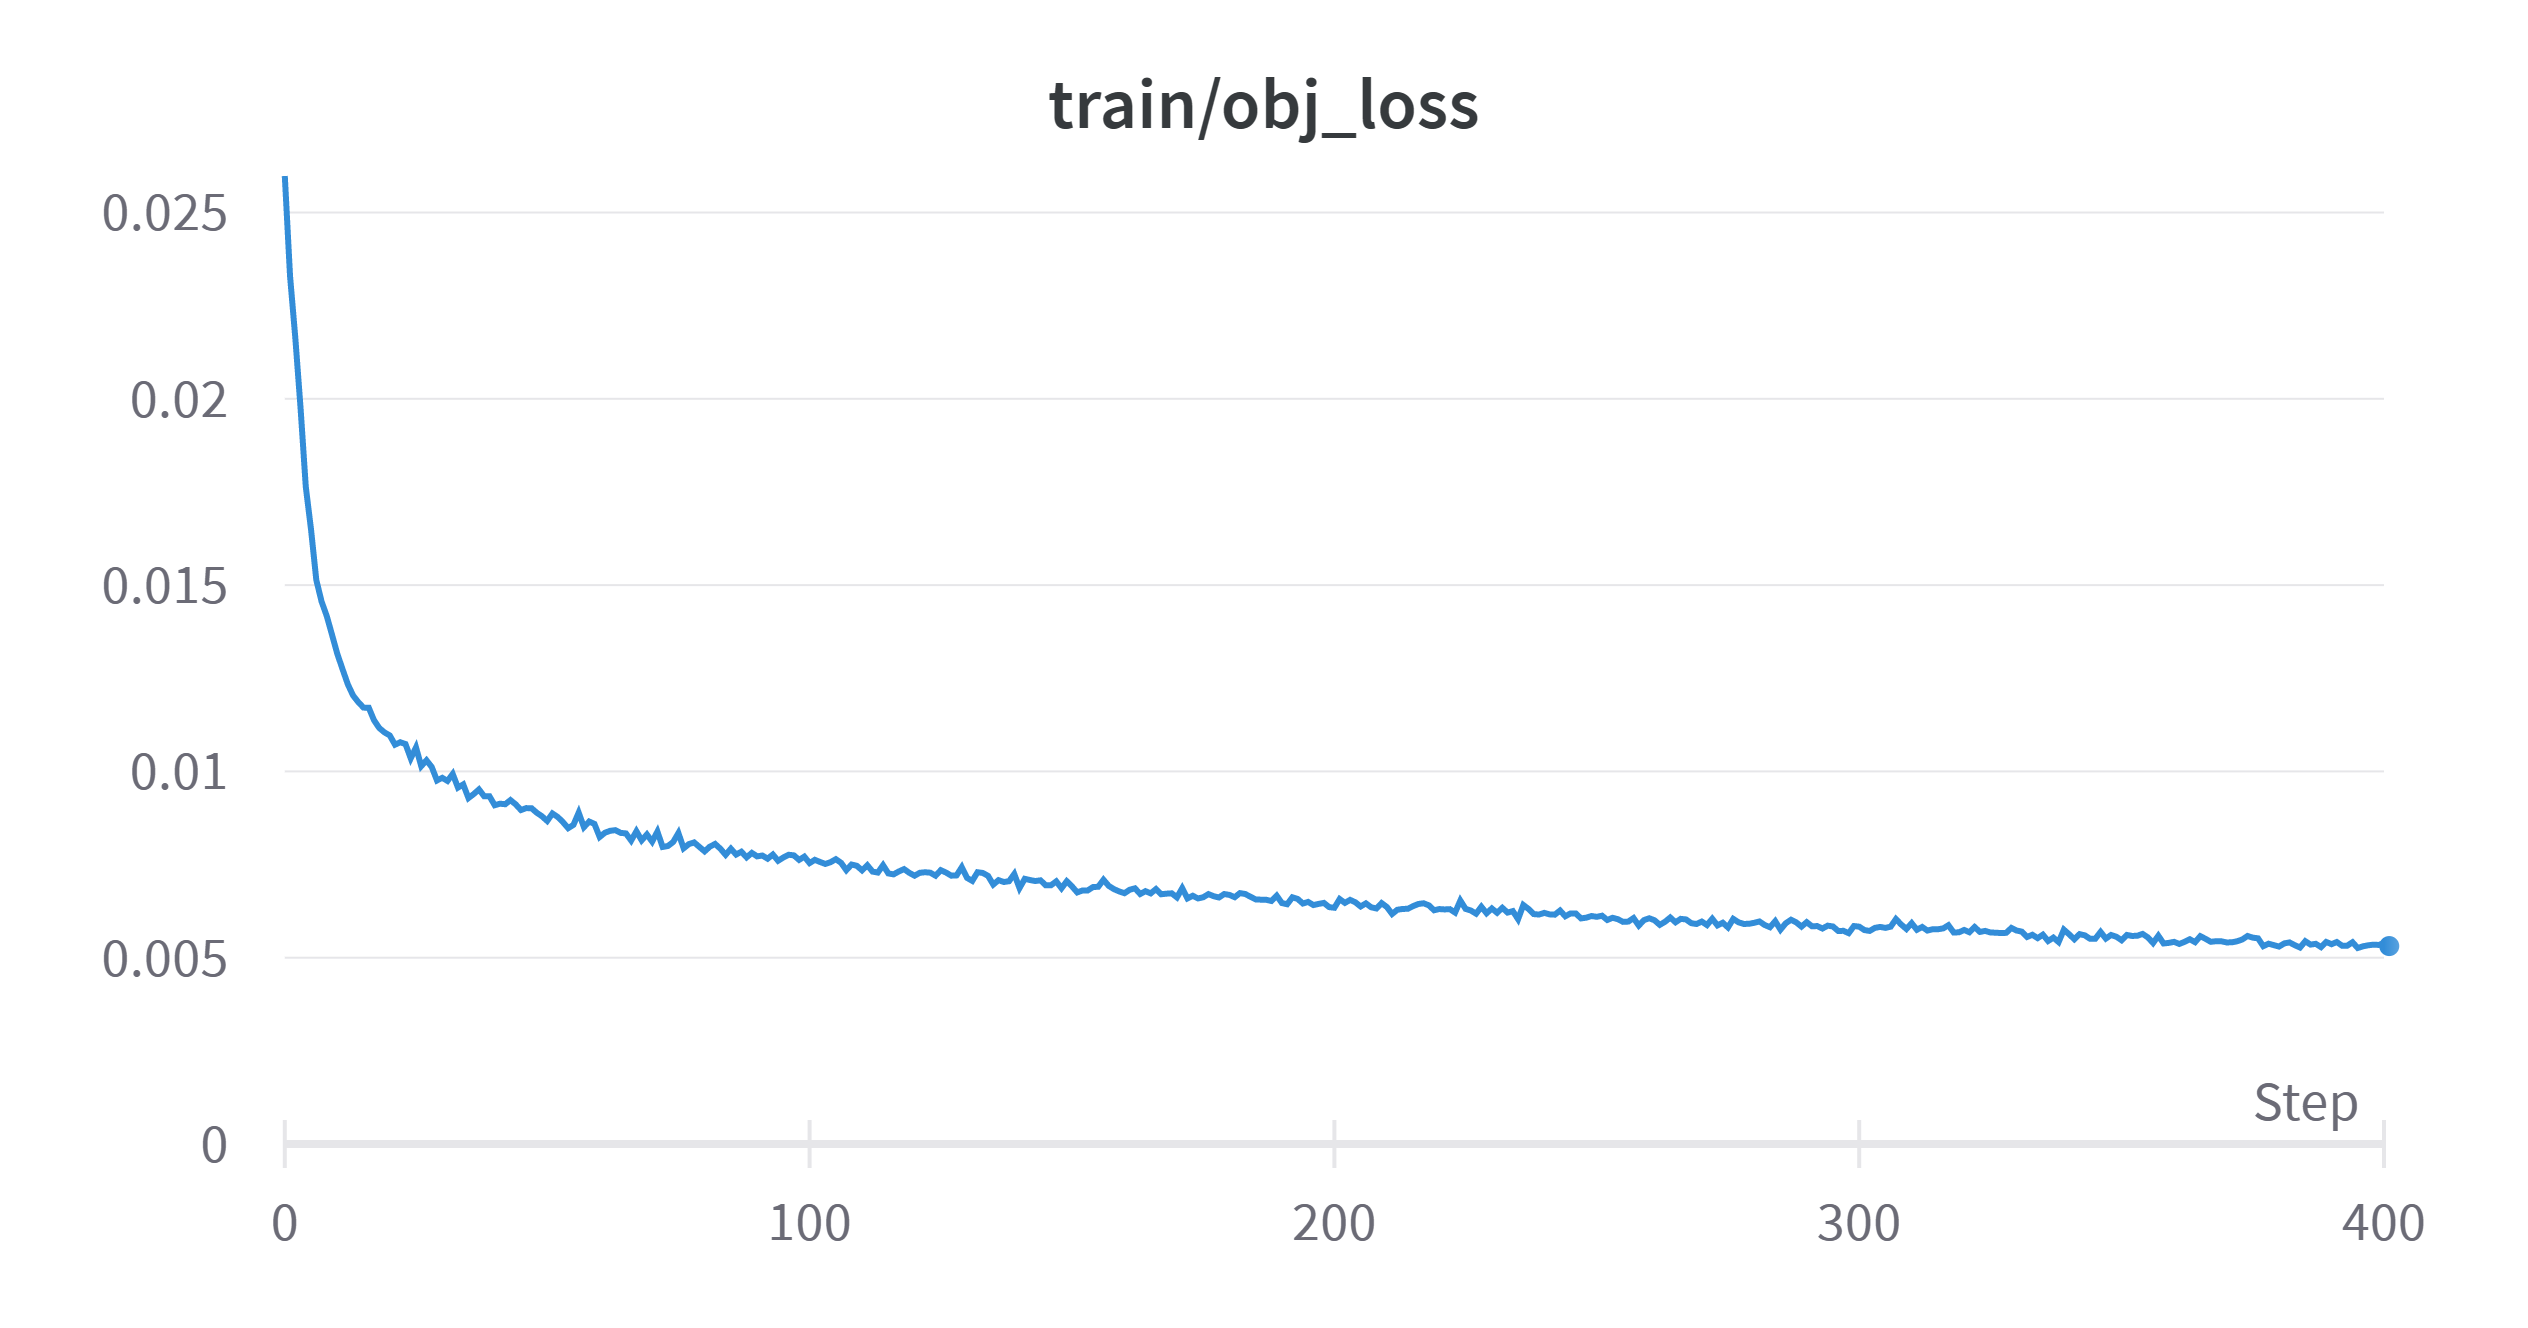
\includegraphics[width=0.95\linewidth]{obrazky-figures/train_obj1.png}\hfill
    \caption{Objectness loss při tréninku}
    \end{subfigure}
    \begin{subfigure}{0.7\textwidth}
    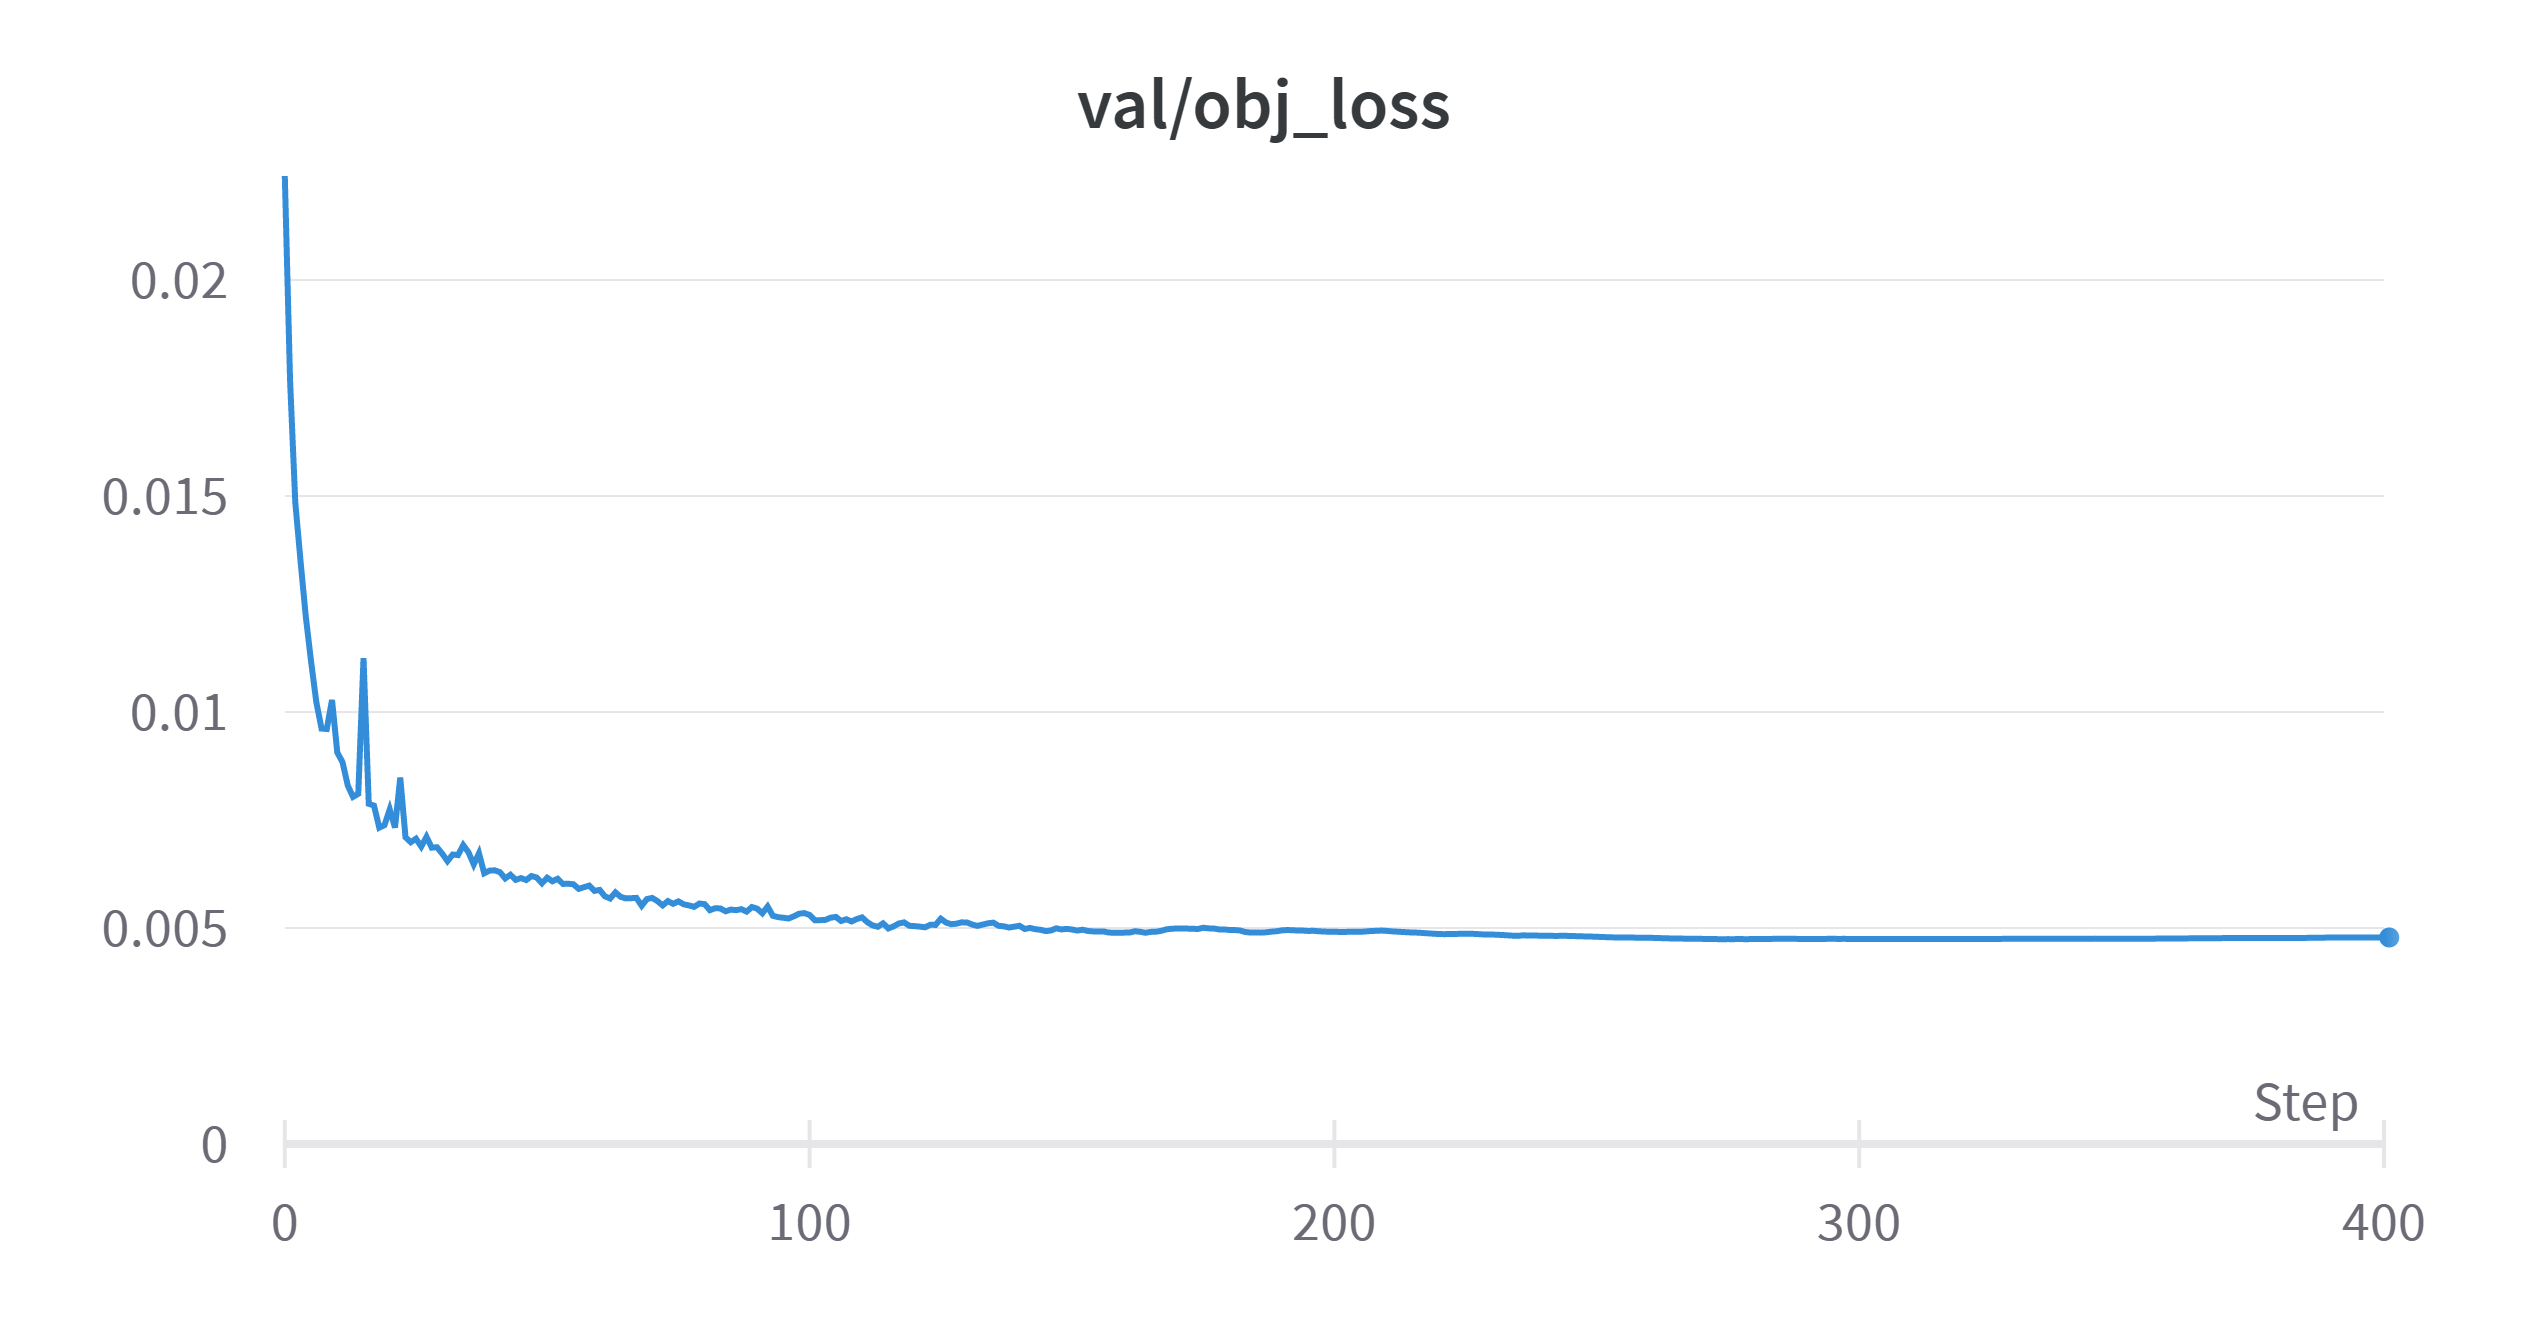
\includegraphics[width=0.95\linewidth]{obrazky-figures/obj_val1.png}\hfill
    \caption{Objectness loss při validaci}
    \end{subfigure}
    \caption{Objectness loss sítě YOLOv5 v jednotlivých epochách. Objectness loss měří rozdíl mezi objectness detekovaného ohraničující boxu a předem definovaného ohraničující boxu. Objectness je pravděpodobnost že se objekt vyskytuje v předpovězeném okně. Čím menší je objectness loss, tím je model přesnější.}
    \label{obj1}
\end{figure}

\paragraph{} Samotný postup učení lze vidět i na metrikách recall, precision a average precision s prahem 0.5. Na grafech \ref{precall1} lze viděl rychlé naučení na jakousi základní úroveň již v sedmi epochách, za kterou následuje pomalejší zdokonalování modelu. Nejlepší hodnoty average precision dosáhl model v epoše 202. V tomto bodě byla average precision 0.9193, recall 0.8899 a precision 0.9013. Je to také epocha kdy byl nejvyšší recall, přičemž u metriky precision můžeme pozorovat zmenšení oproti předchozí epoše, kdy byla precision 0.914.
\pagebreak

\begin{figure}[h]\centering
    \centering
    \begin{subfigure}{0.6\textwidth}
    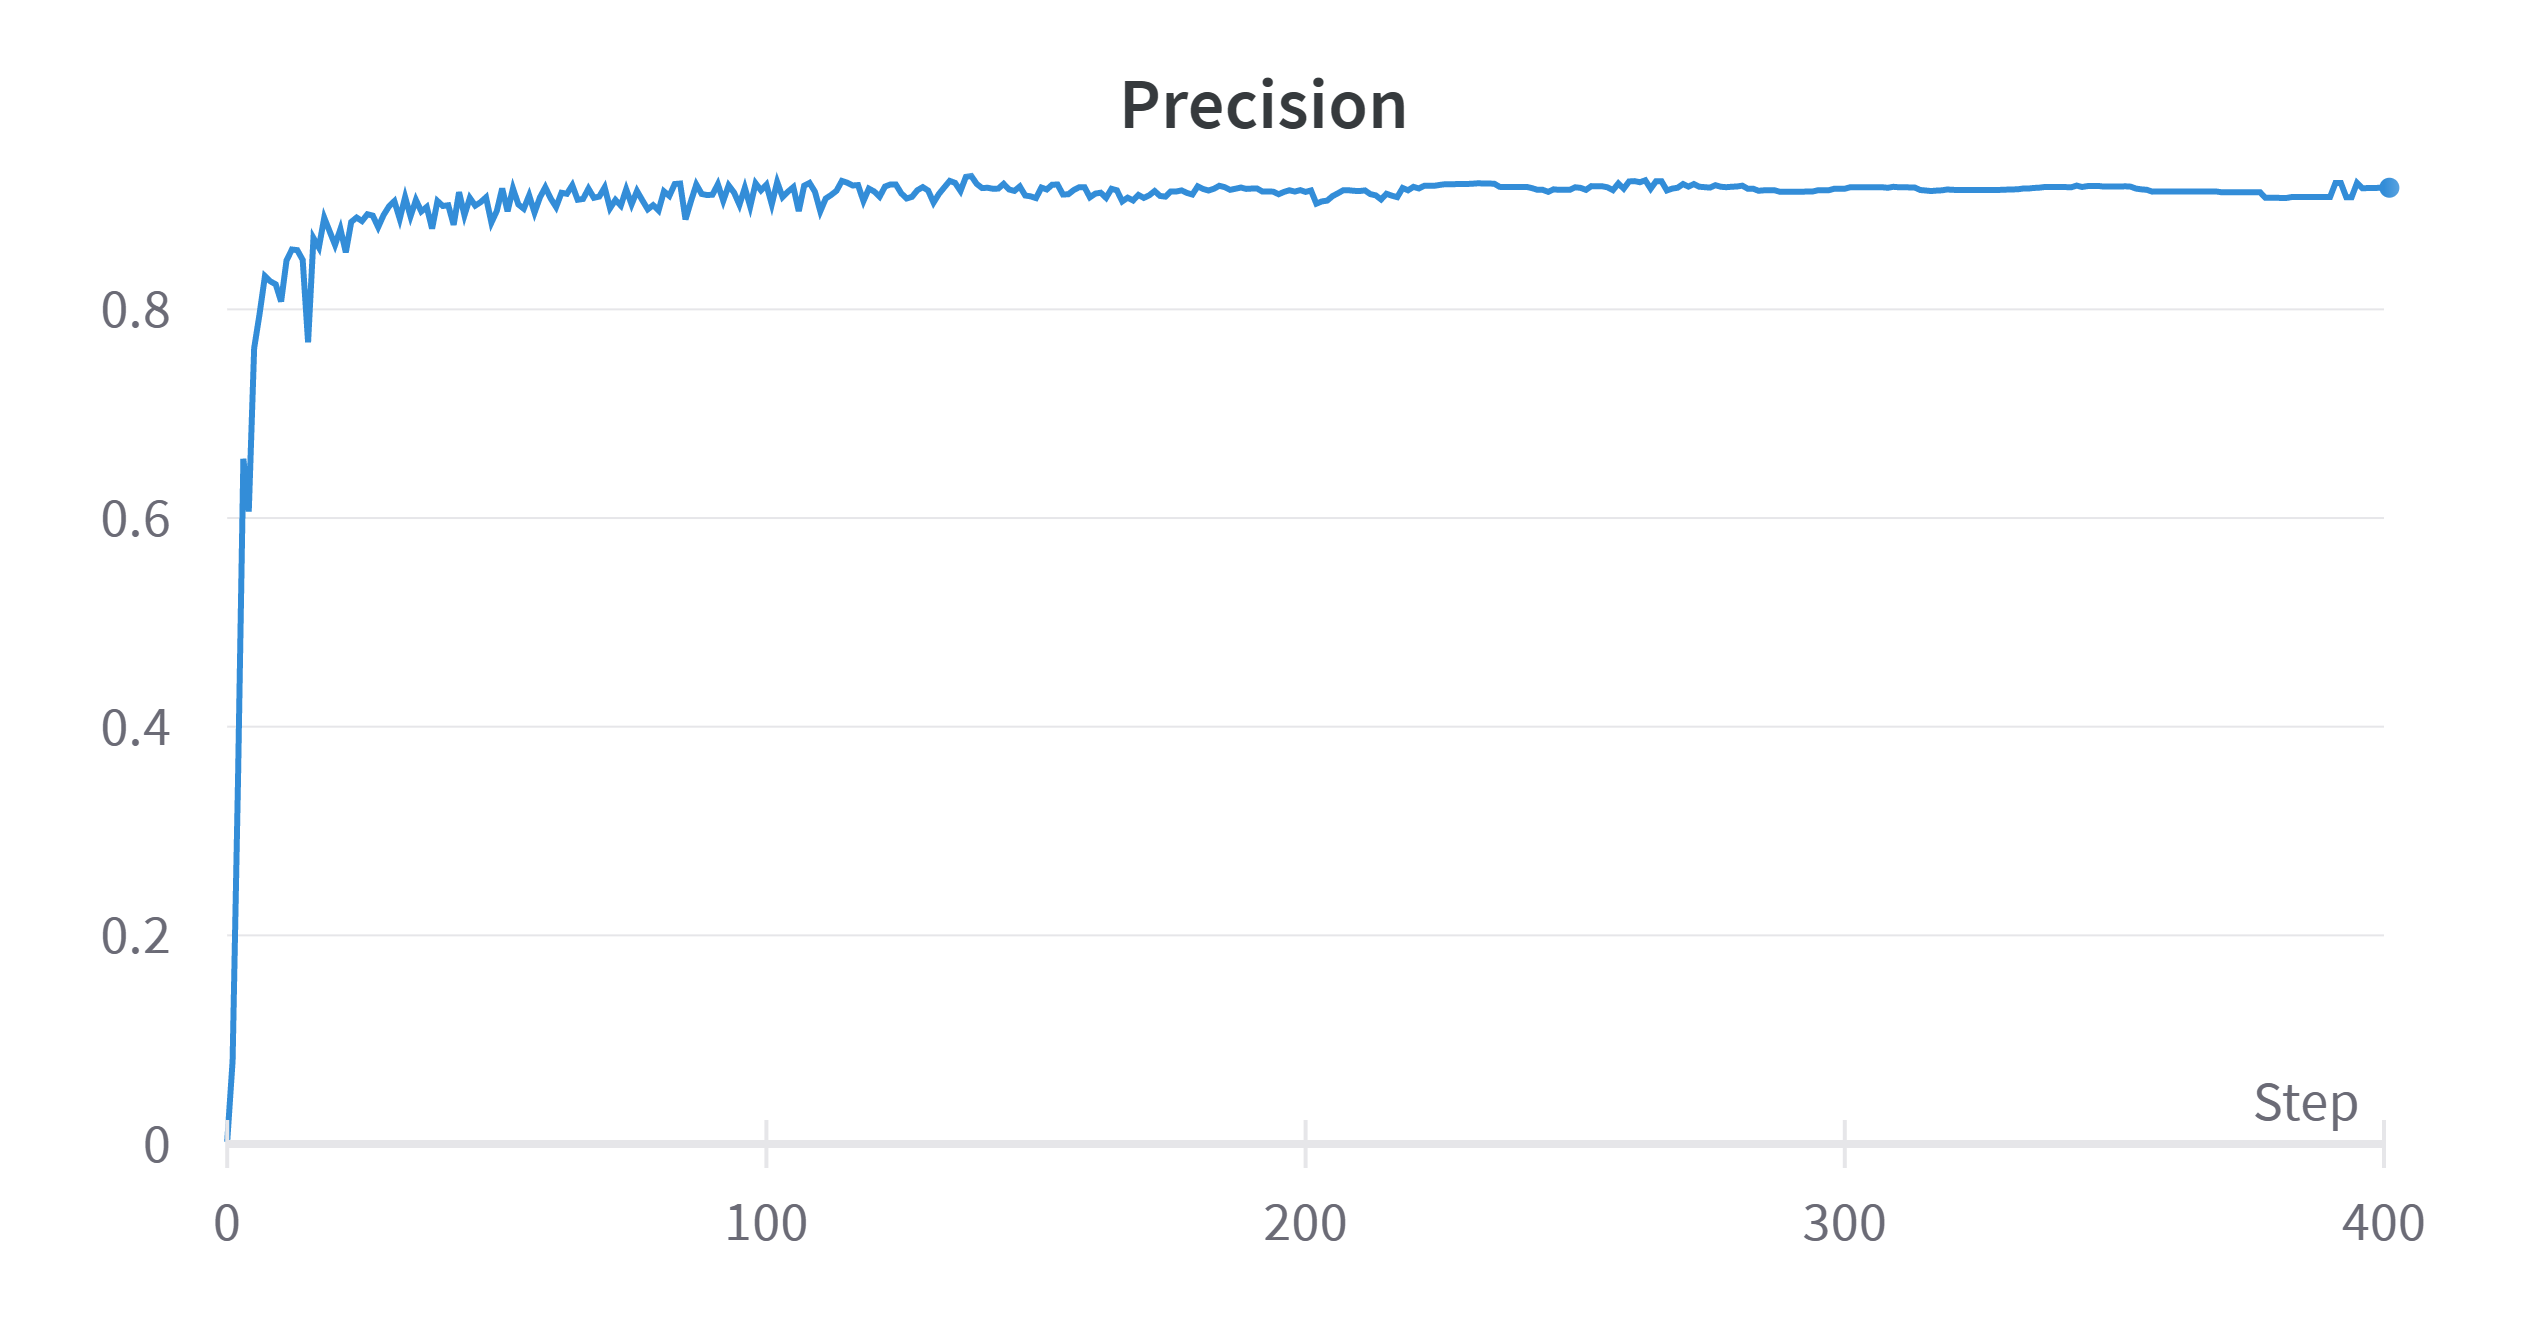
\includegraphics[width=0.95\linewidth]{obrazky-figures/wbprecision.png}\hfill
    \caption{Precision v jednotlivých epochách}
    \end{subfigure}
    \begin{subfigure}{0.6\textwidth}
    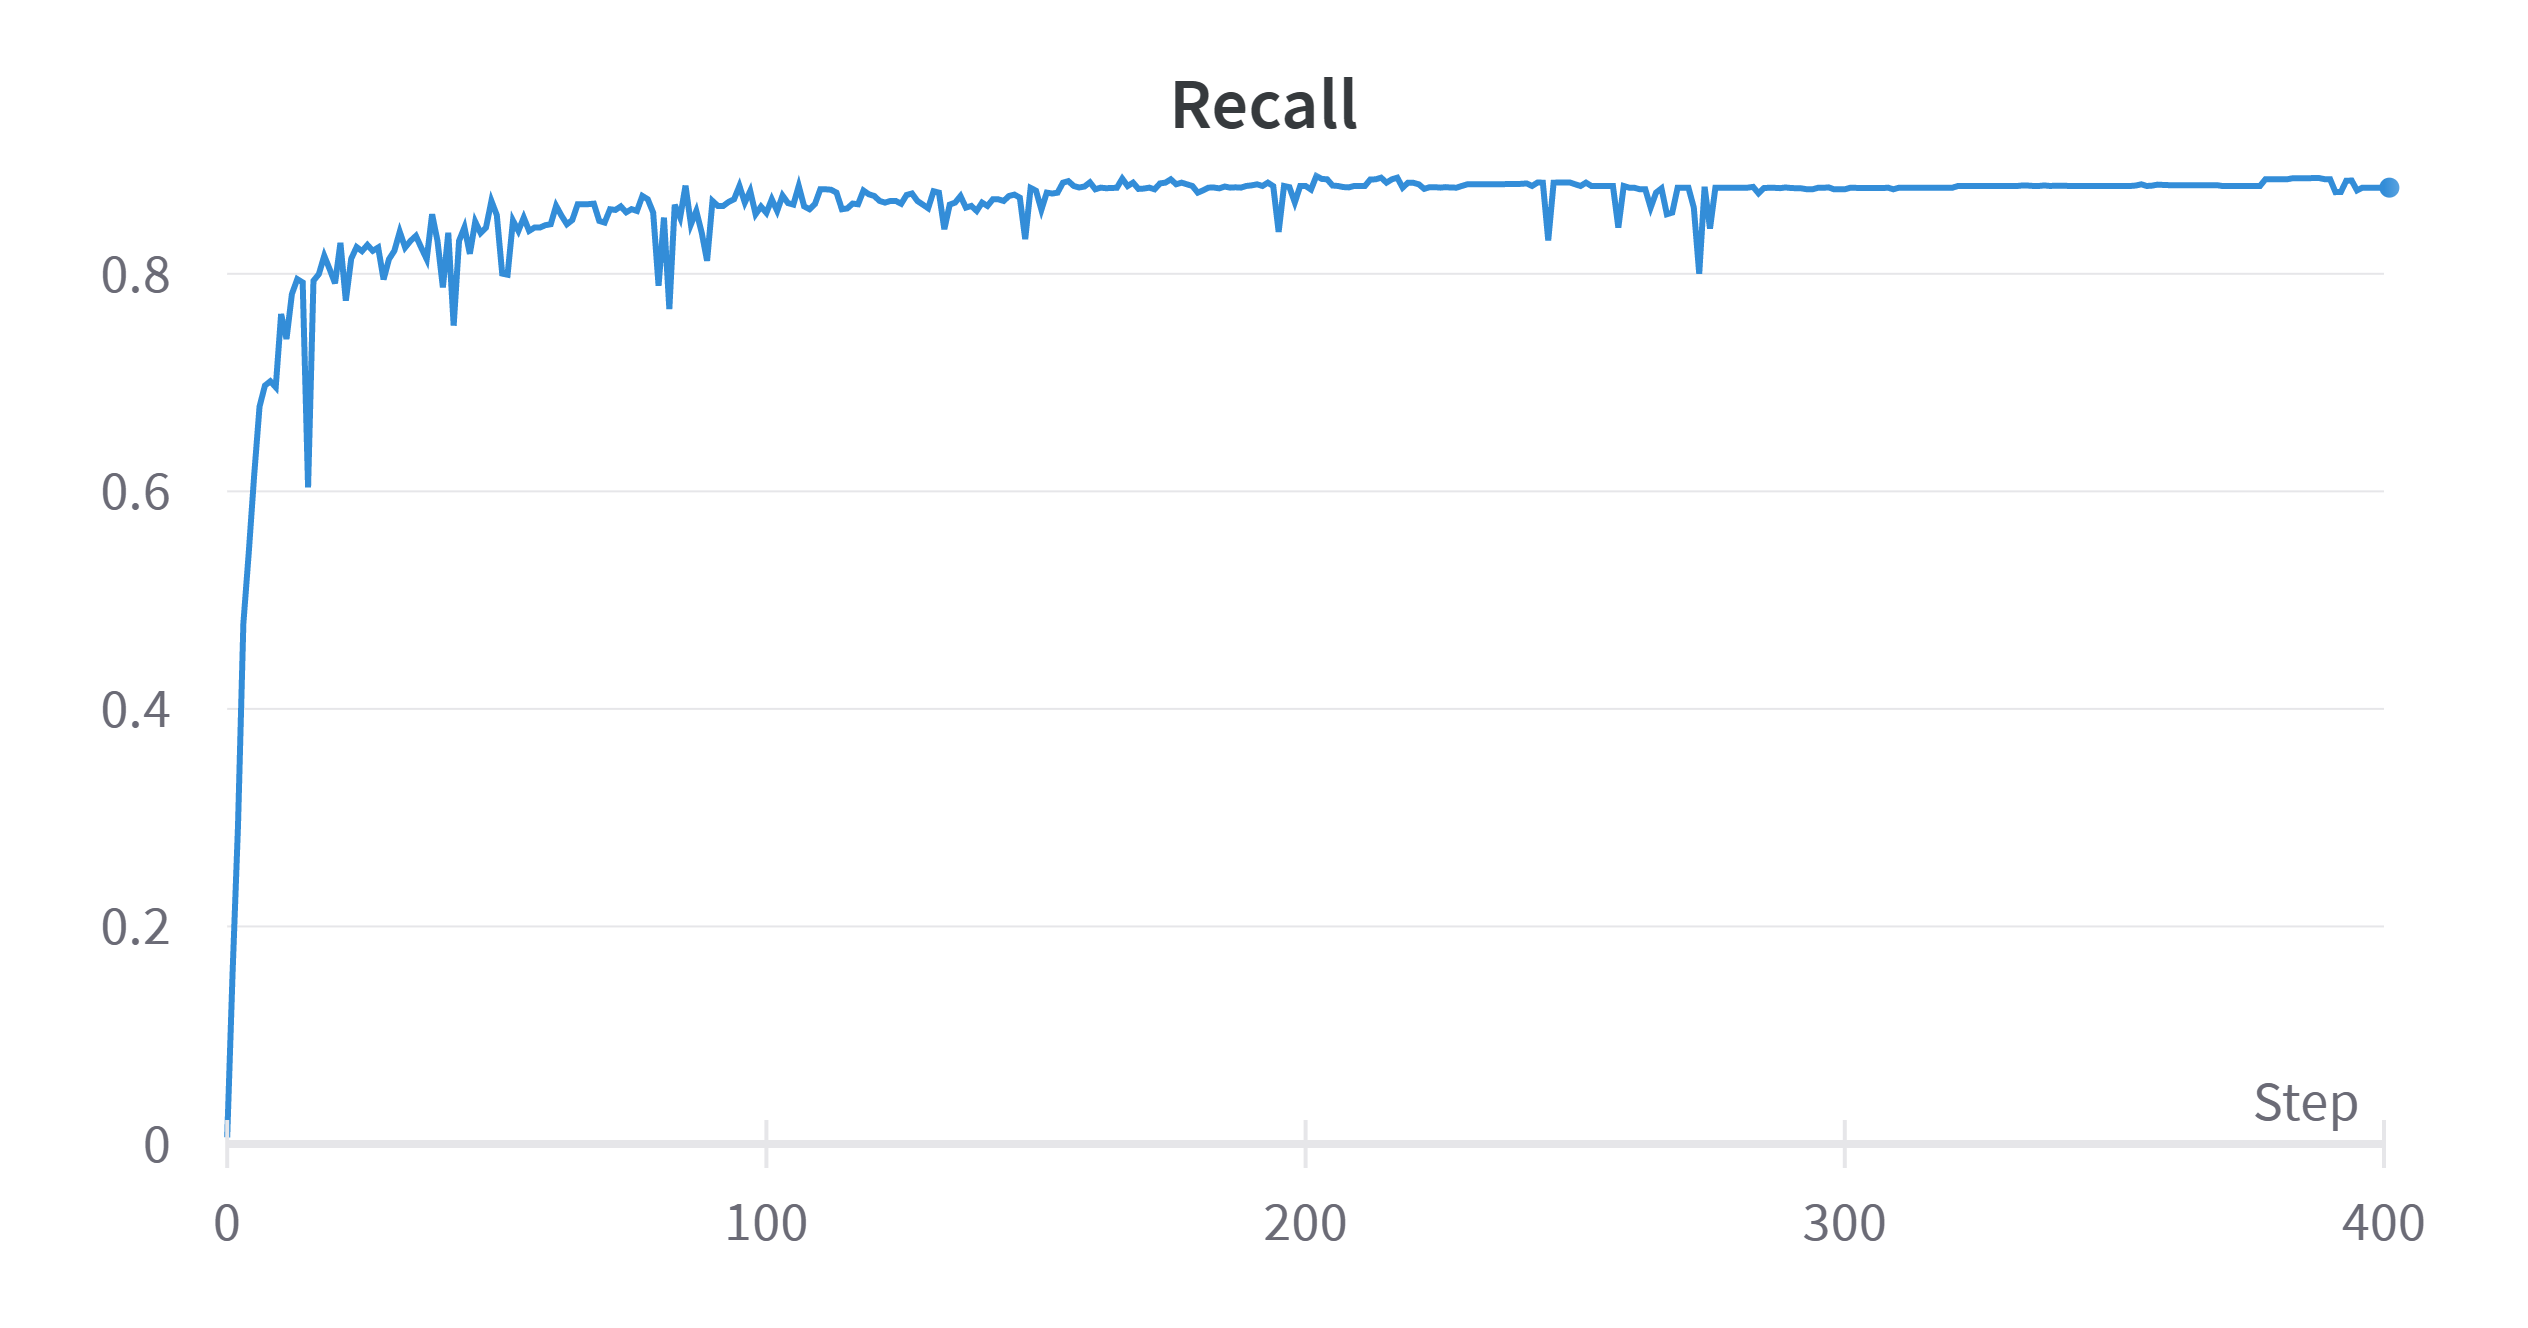
\includegraphics[width=0.95\linewidth]{obrazky-figures/wbrecall.png}\hfill
    \caption{Recall v jednotlivých epochách}
    \end{subfigure}
    \begin{subfigure}{0.6\textwidth}
    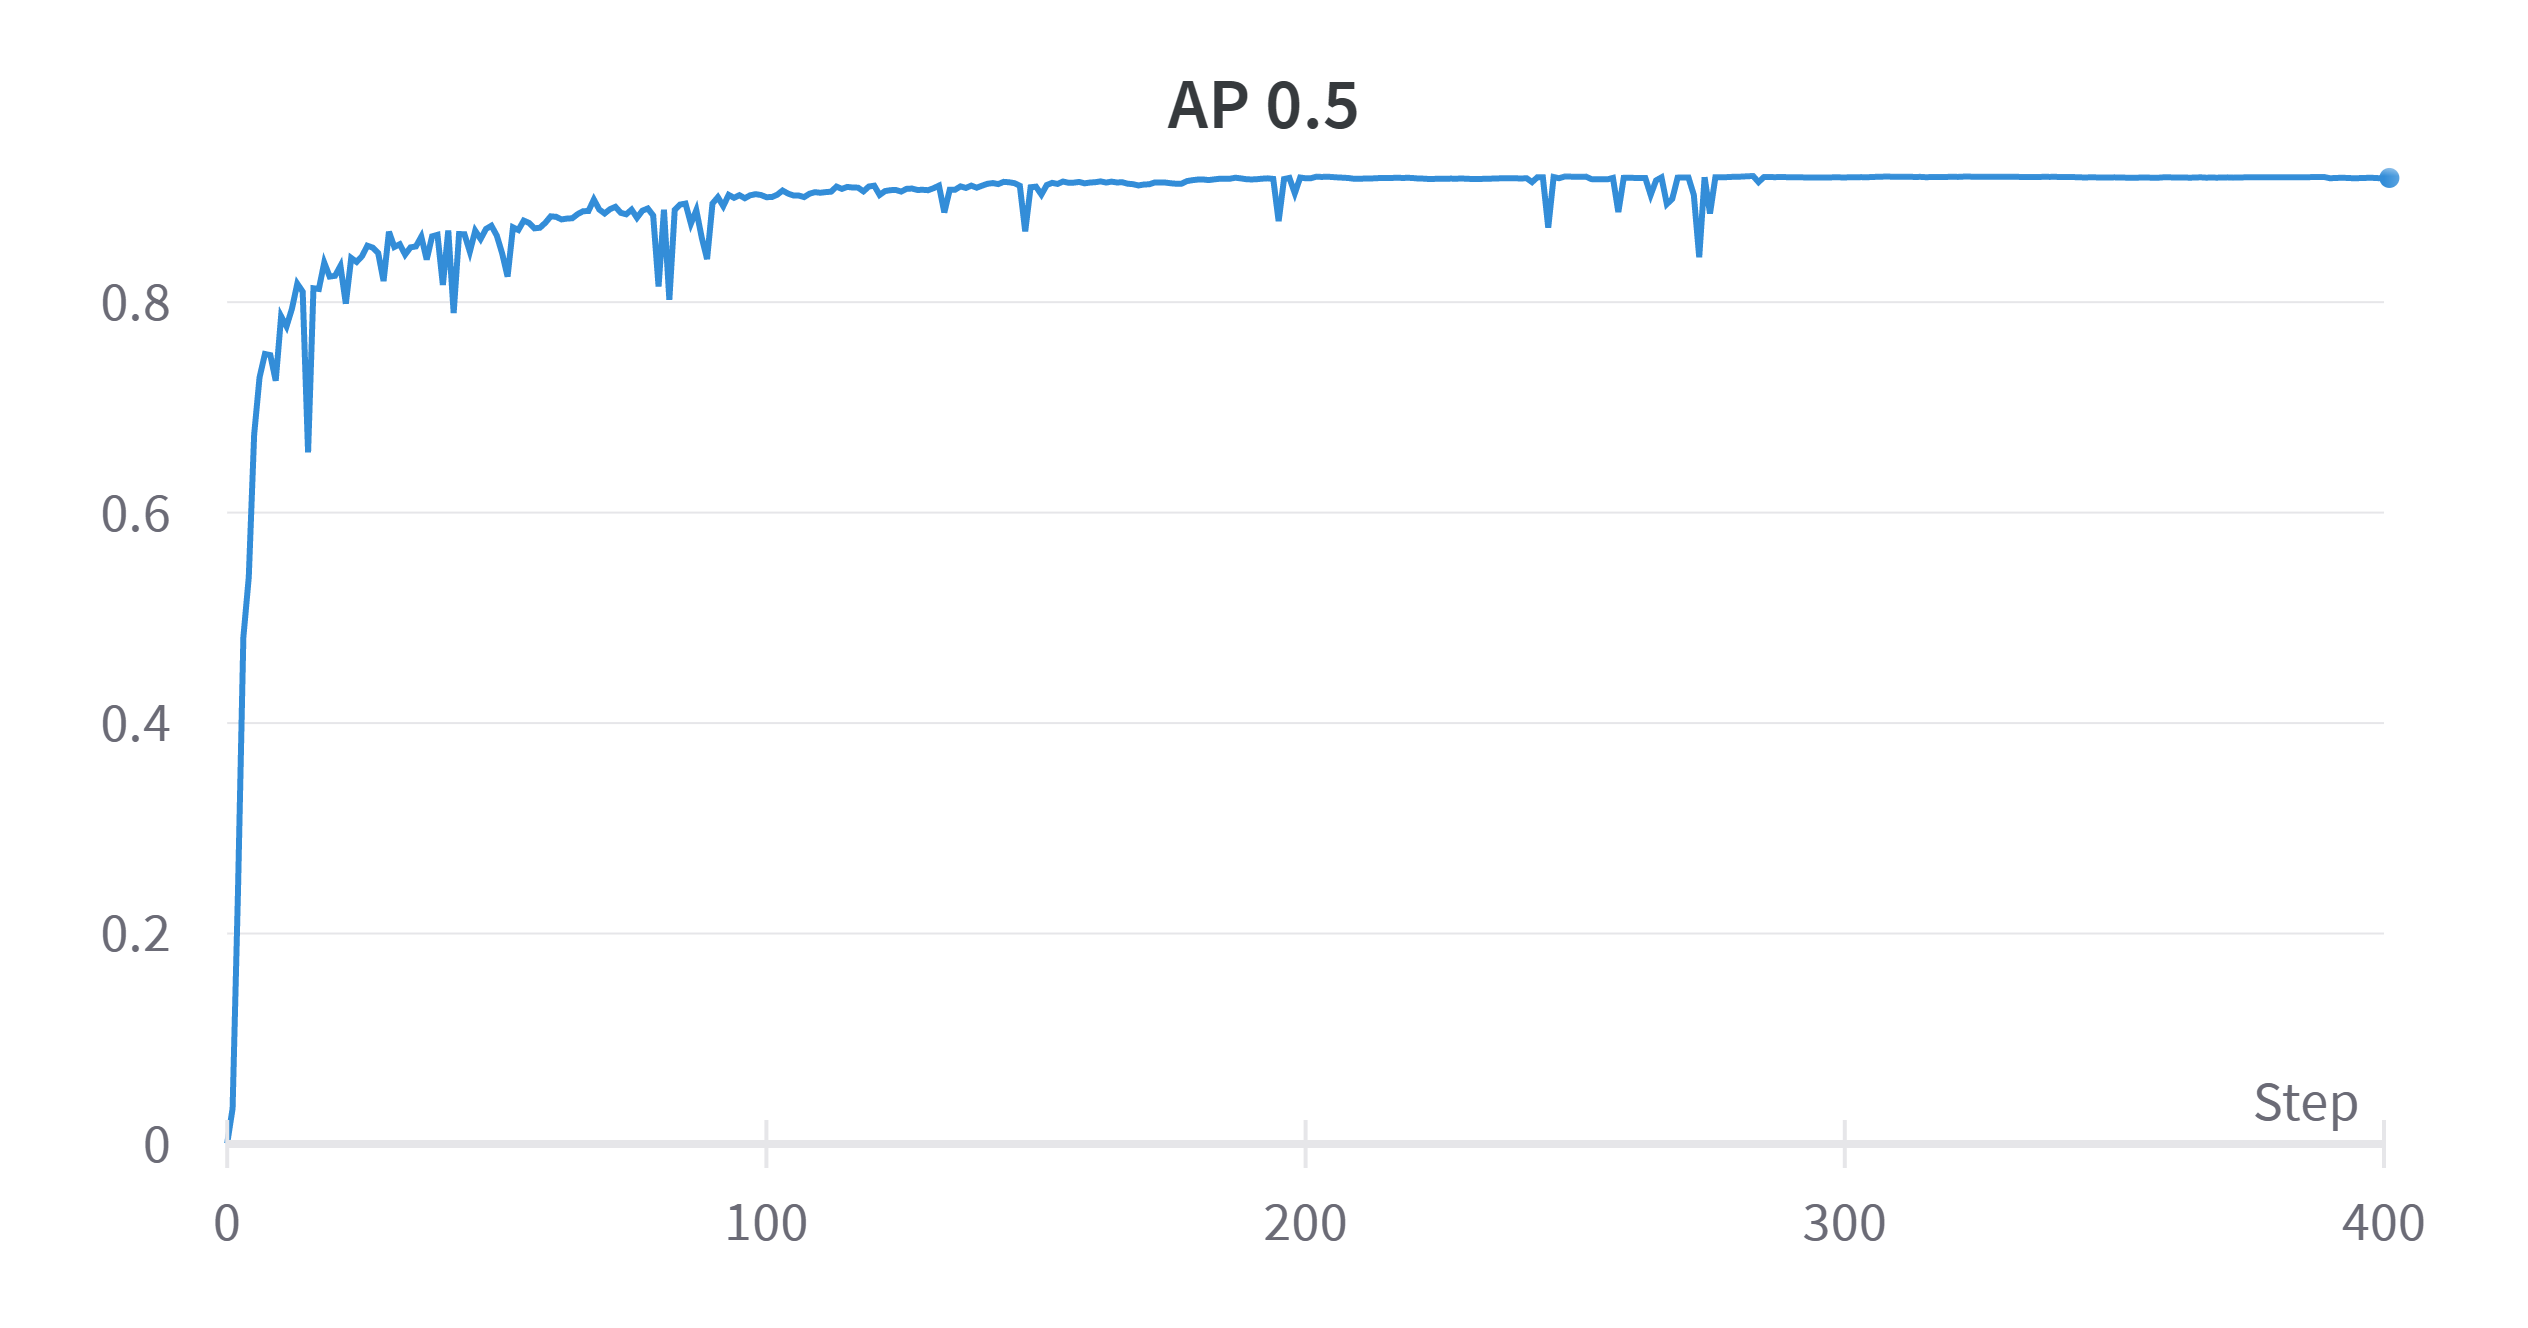
\includegraphics[width=0.95\linewidth]{obrazky-figures/wbap.png}\hfill
    \caption{Average precision s prahem 0.5 v jednotlivých epochách}
    \end{subfigure}
    \caption{Na grafech lze vidět různé metriku v průběhu času. Lze zřetelně vidět proces učení a to i s poklesem v 15. epoše. Čím vyšší jsou tyto metriky tím lépe model detekuje čárové kódy.}
    \label{precall1}
\end{figure}
\pagebreak

Při konečném testování učení neuronové sítě na testovací části sady, se ukázal přijatelný propad. Average precision bylo 0.8937, což představuje propad o 0.0256. 

\paragraph{} Finální testovaní jsem provedl stejně jako u předchozích metod \ref{scharr_exp} a \ref{opencv_exp} na orientovaném datasetu s hodnotami prahů 0.5, 0.75 a 0.9. Jelikož je tato metoda vytvořená a vytrénovaná na detekci neorientovaných ohraničujících boxů, výsledky této části testovaní jsou o poznání méně uspokojivé než u předchozích částí.
\paragraph{} Při testování na celém datasetu, včetně částí na kterých byla síť trénována, dosáhla metoda při prahu 0.5 average precision 0.6624, recall 0.9811, precision 0.7287 a f1 skóre bylo 0.8362. Jak lze vidět jediný recall zůstal vysoký, dokonce vyšší než u samotného trénování. Je to způsobeno tím, že u dat, na kterých byla síť trénována, je kvalita detekce vyšší. Zároveň i přes orientaci předem definovaných dat, se čárové kódy stále vyskytují v detekovaném ohraničujícím boxu, i když intersection over union není tak vysoké.
\paragraph{} Při zvýšení prahu na hodnoty 0.75 a 0.9 lze pozorovat značné zmenšení všech metrik kromě recallu. Na úrovni prahu 0.75 je average precision 0.3056, recall 0.9598, precision 0.3362 a f1 skóre  0.4979. Z vyšším prahem 0.9 se metriky nadále snižují. Average precision se sníží na 0.0918, recall na hodnotu 0.8885, precision se sníží na 0.1122 a f1 skóre na 0.1992. Toto snižování je logické, protože kvůli rozdílu v orientaci mezi detekovanými ohraničujícími boxy a předem definovanými ohraničujícími boxy je intesection over union nízké.
\paragraph{} Lze také pozorovat zásadní změny mezi aliasovanou částí datasetu a nealiasovanou částí. Při prahu 0.5 je average precision aliasované části 0.5967, recall 0.9612, precision 0.6564 a f1 skóre 0.7801. U nealiasované části je average precision roven 0.7035, recall  0.9919, precision 0.7739 a f1 skóre 0.8695. Na hladinách prahu 0.75 a 0.9 je situace obdobná jak lze pozorovat v tabulce \ref{yolov5_table}. Průměrná rychlost detekce je 0.1277 vteřina na jeden detekovaný čárový kód.


\begin{table}[ht]
\centering
\begin{tabular}{|l|c|c|c|c|}
\hline
Práh - dataset     & Average precision & Recall  & Precision & F1      \\ \hline
0.5 - aliased & 0.5967 & \multicolumn{1}{l|}{0.9612} & \multicolumn{1}{l|}{0.6564} & \multicolumn{1}{l|}{0.7801} \\ \hline
0.5 - not aliased  & 0.7035          & 0.9919 & 0.7739  & 0.8694 \\ \hline
0.5 - combined     & 0.6624           & 0.9811 & 0.7287    & 0.8362 \\ \hline
0.75 - aliased     & 0.2388             & 0.9083  & 0.2626    & 0.4074  \\ \hline
0.75 - not aliased & 0.3475            & 0.9838 & 0.3822  & 0.5506 \\ \hline
0.75 - combined    & 0.3056            & 0.9598 & 0.3362   & 0.4979  \\ \hline
0.9 - aliased      & 0.0456               & 0.7028     & 0.0627       & 0.1151     \\ \hline
0.9 - not aliased  & 0.1301               & 0.9579     & 0.1431       & 0.249     \\ \hline
0.9 - combined     & 0.0918               & 0.8885     & 0.1122       & 0.1992     \\ \hline
\end{tabular}
\caption{V této tabulce jsou přehledně zapsány naměřené metriky detektoru čárových kódů založeném na neuronové síti YOLOv5.}
\label{yolov5_table}
\end{table}

\pagebreak

\begin{figure}[h]\centering
    \centering
    \begin{subfigure}{0.9\textwidth}
    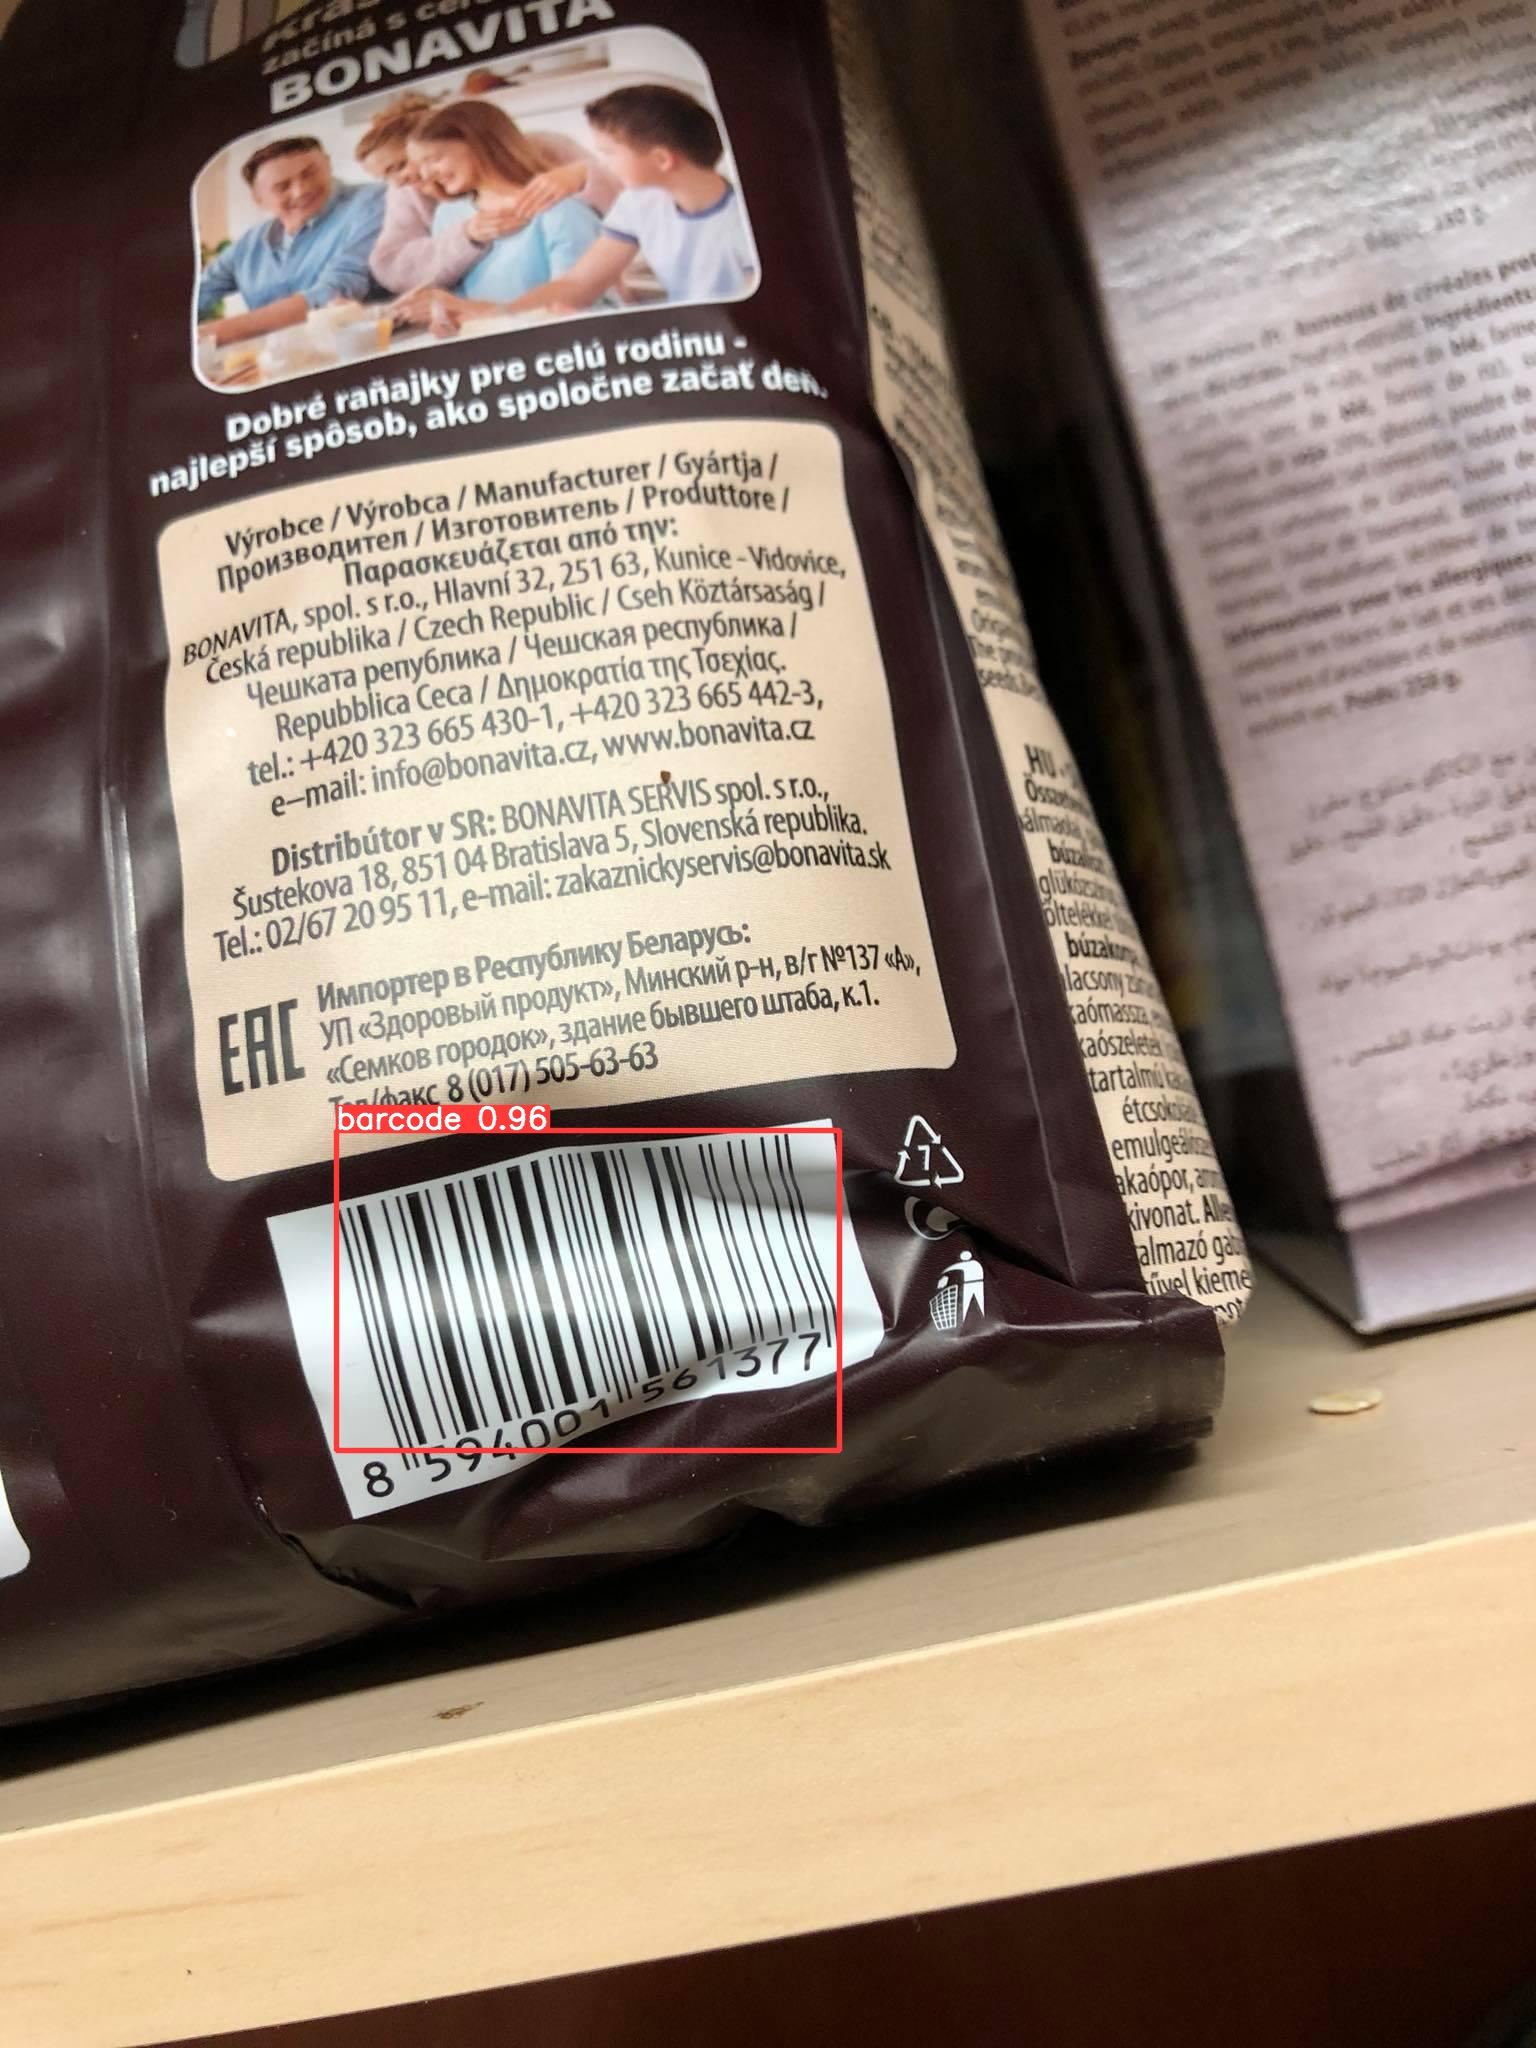
\includegraphics[width=0.45\linewidth]{obrazky-figures/yolo3.jpg}\hfill
    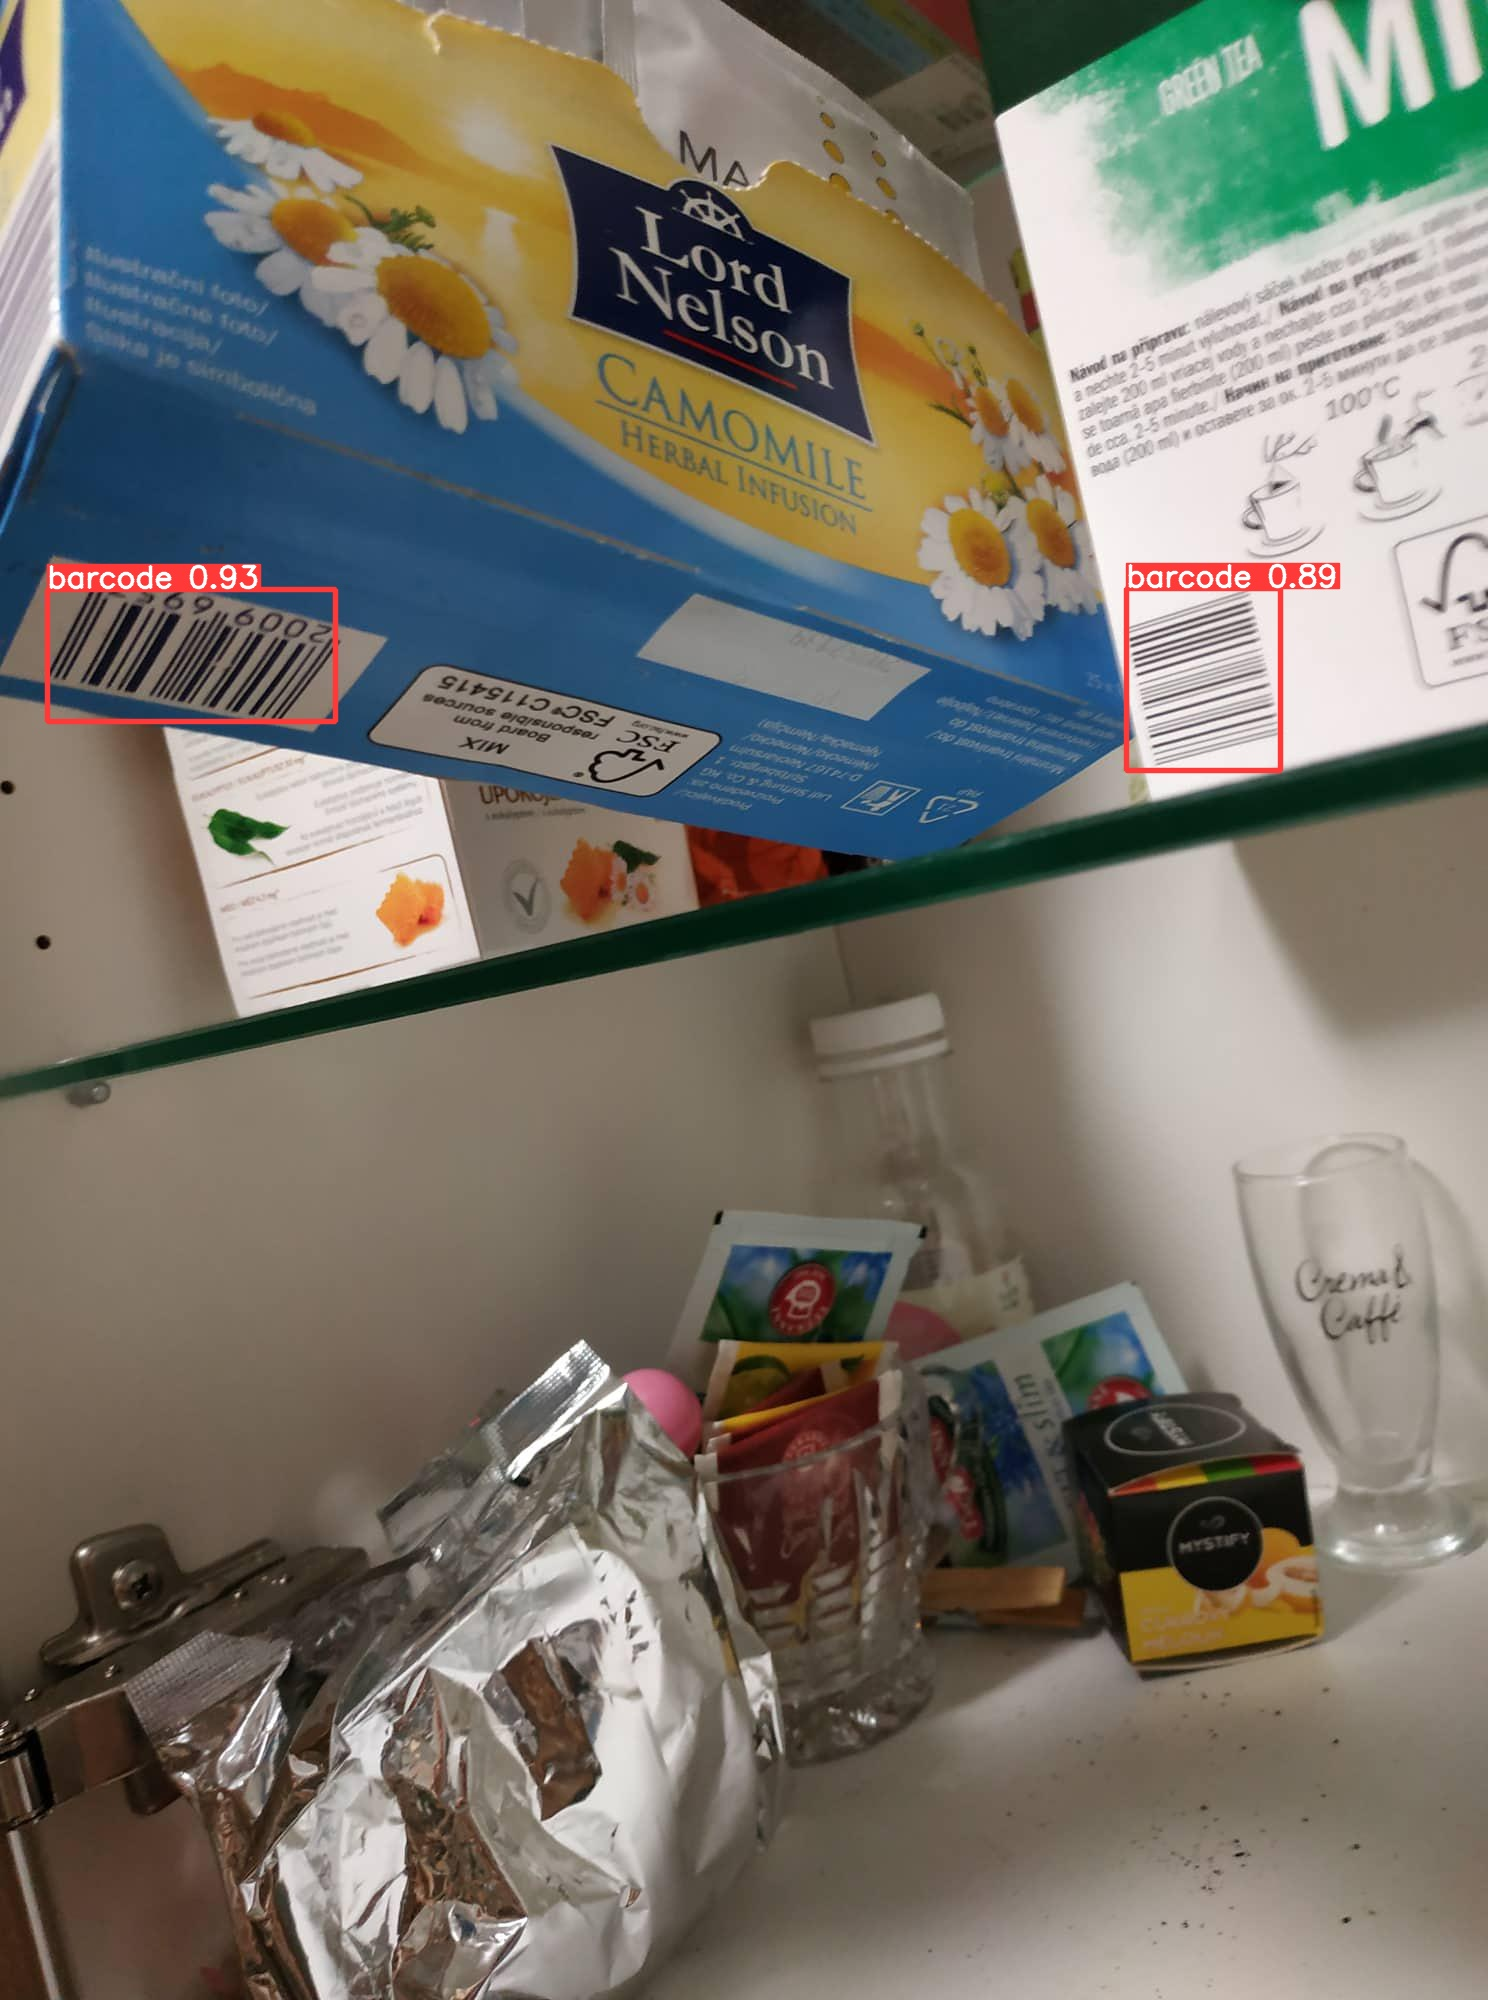
\includegraphics[width=0.45\linewidth]{obrazky-figures/yolo2.jpg}\hfill
    \end{subfigure}
    \begin{subfigure}{0.9\textwidth}
    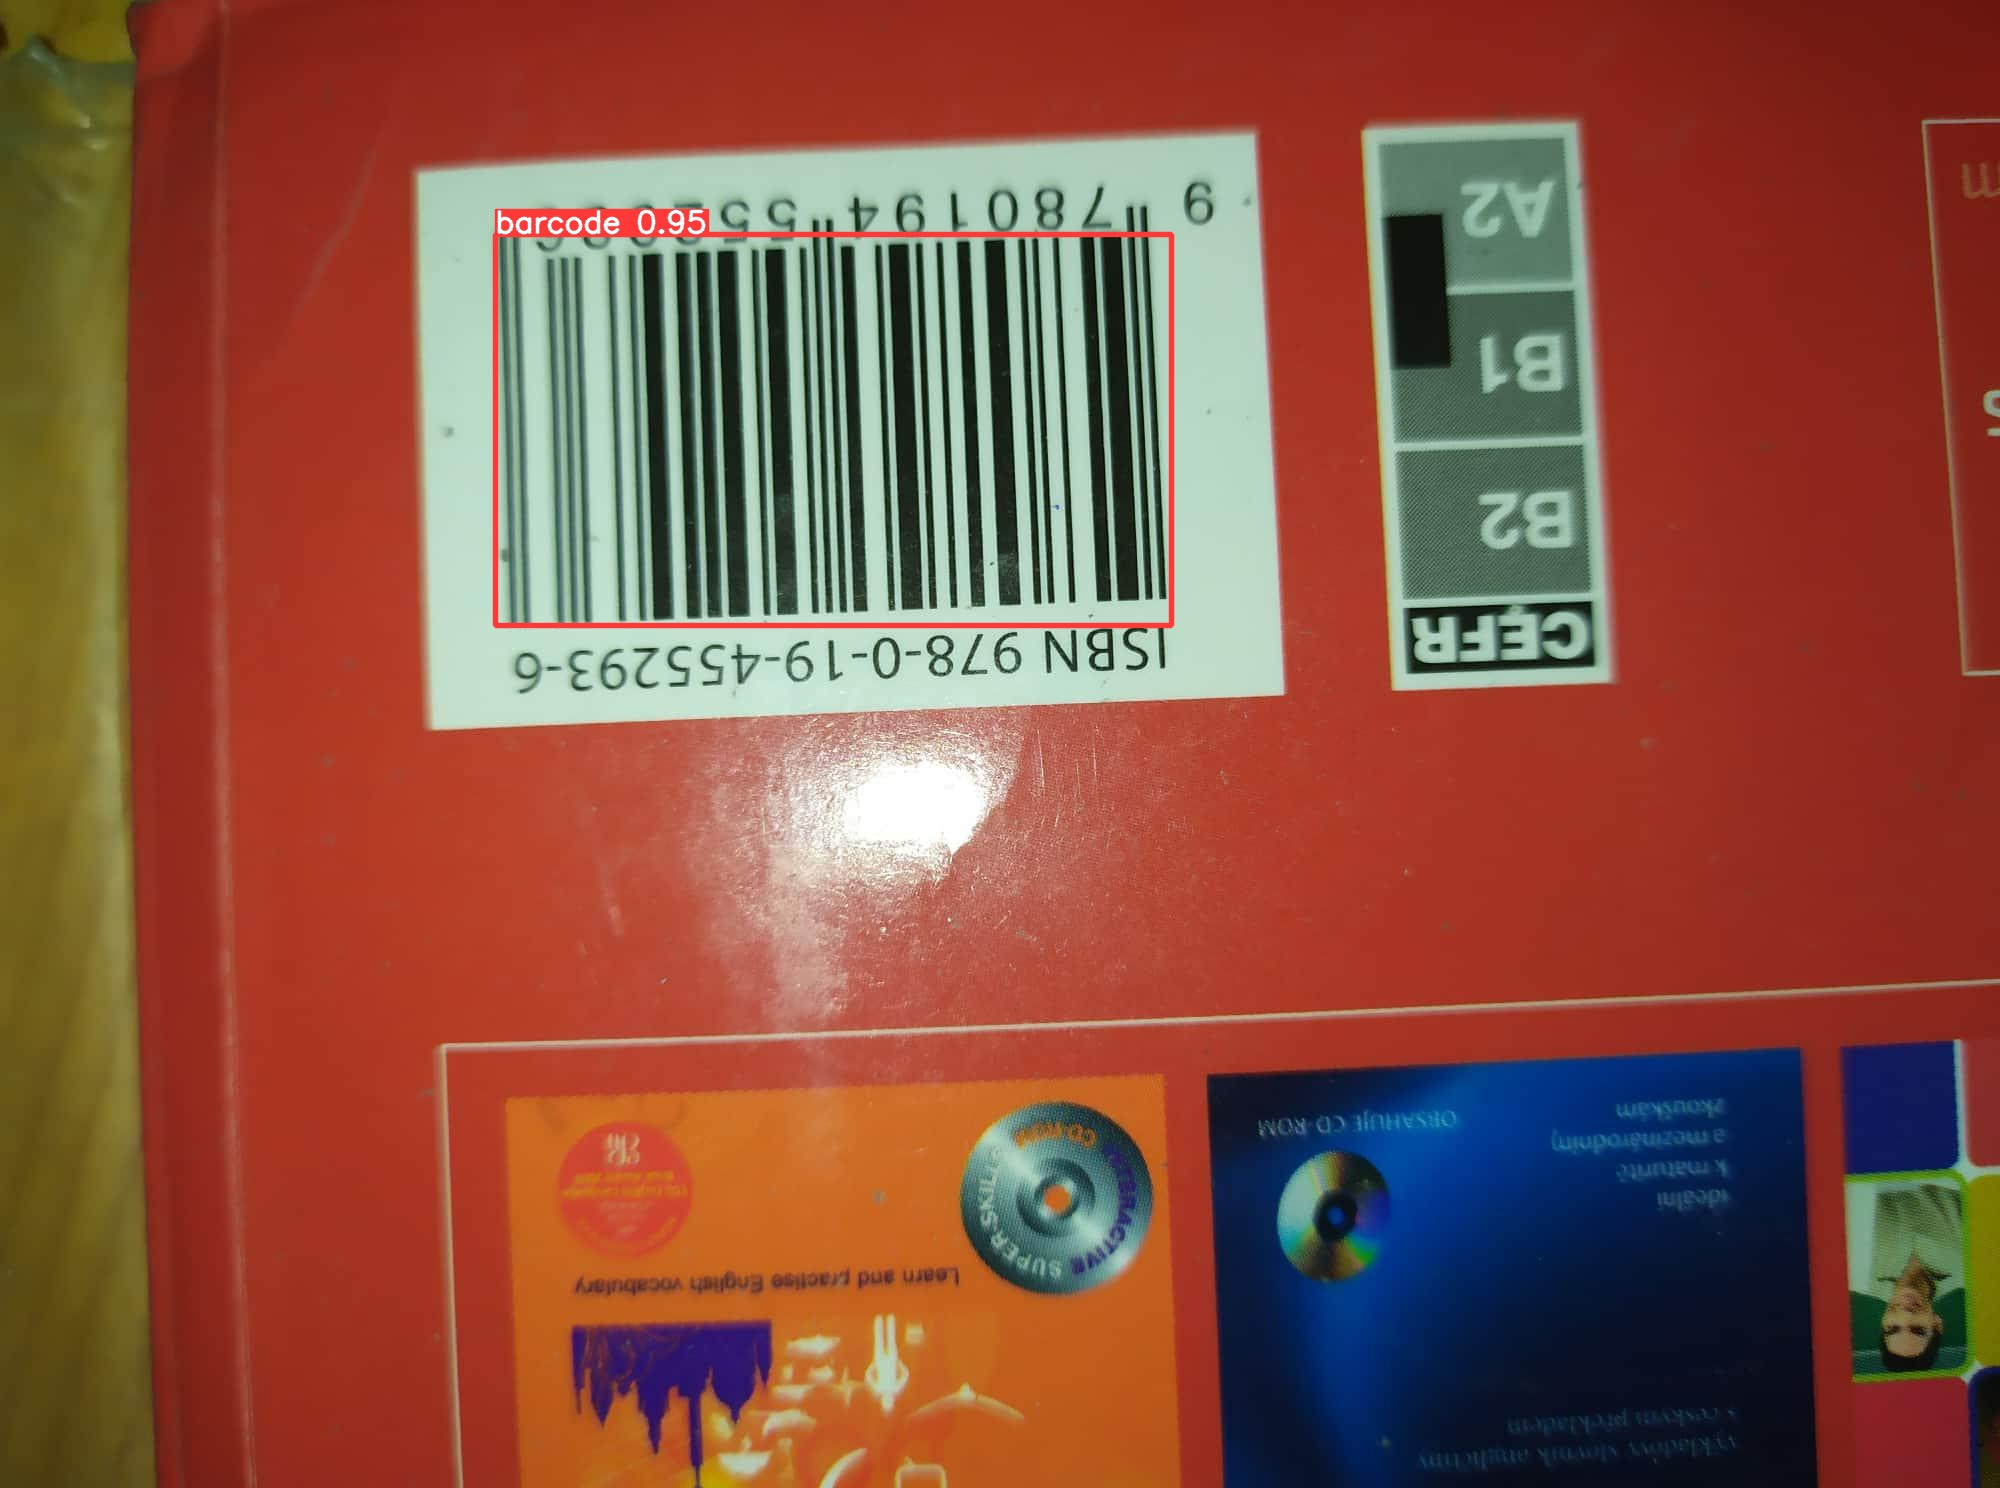
\includegraphics[width=0.45\linewidth]{obrazky-figures/yolo1.jpg}\hfill
    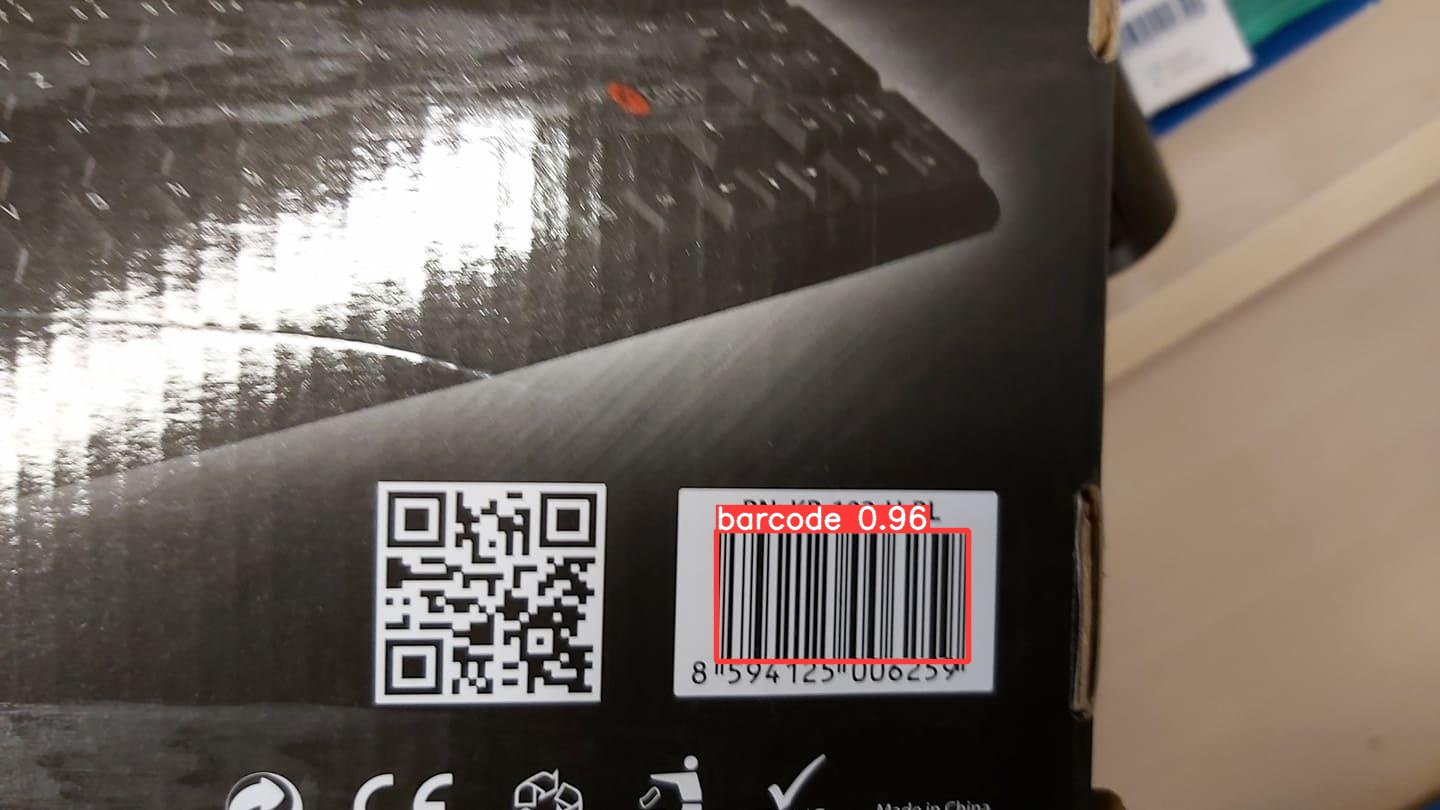
\includegraphics[width=0.45\linewidth]{obrazky-figures/yolo4.jpg}\hfill
    \end{subfigure}
    \caption{Příklady detekce umělé neuronové sítě YOLOv5. Nápis barcode představuje třídu objektu a číslo vedle tohoto nápisu představuje confidence score. To značí pravděpodobnost s jakou je detekovaný objekt opravdu čárový kód.}
    \label{precall2}
\end{figure}

 

\chapter{Návrh, implementace a zhodnocení metody detekce čárových kódů} 
\label{implementation}

Návrh metody kombinuje metodu detekce YOLOv5 \cite{yolov5_github} a detektor čárových kódů knihovny OpenCV \cite{opencv_barcode}. Zároveň jsem implementoval počítání metrik jako average precision, recall, precision a skóre f1. 
\section{Implementace navržené metody}
\subsection*{Detekce}
Program nejprve spustí detekci pomocí YOLOv5 stejným příkazem jako v příkazové řádce, která vygeneruje štítky neorientovaných detekovaných ohraničujících boxů a také jejich výřezi z obrázku. Poté program načte adresář, ze kterého čerpá obrázky pro detekci. Nad tímto adresářem spustí cyklus, ve kterém načte obrázek určený pro detekci, všechny štítky detekované v tomto pomocí YOLOv5 a všechny předem definované štítky v tomto obrázku.
\paragraph{} Následně začne program cyklit nad detekovanými štítky. Jelikož se v obrázcích může vyskytovat více čárových kódů, nejprve se v tomto cyklu zkotroluje, zda jméno souhlasí se jménem výřezu detekovaného čárového kódu. Tyto výřezi jsou pojmenovány stejně jako originál, akorát pokud je výřezků více než jeden, přídá se nakonec číslovka pořadí kromě jedničky. Toto se zkontroluje pomocí proměnné \texttt{i}, která pouze indikuje číslo výřezku a obnovuje se na hodnotu jedna pro každý obrázek.
\begin{figure}[htbp]
    \centering
    \begin{subfigure}{0.7\textwidth}
    \centering
    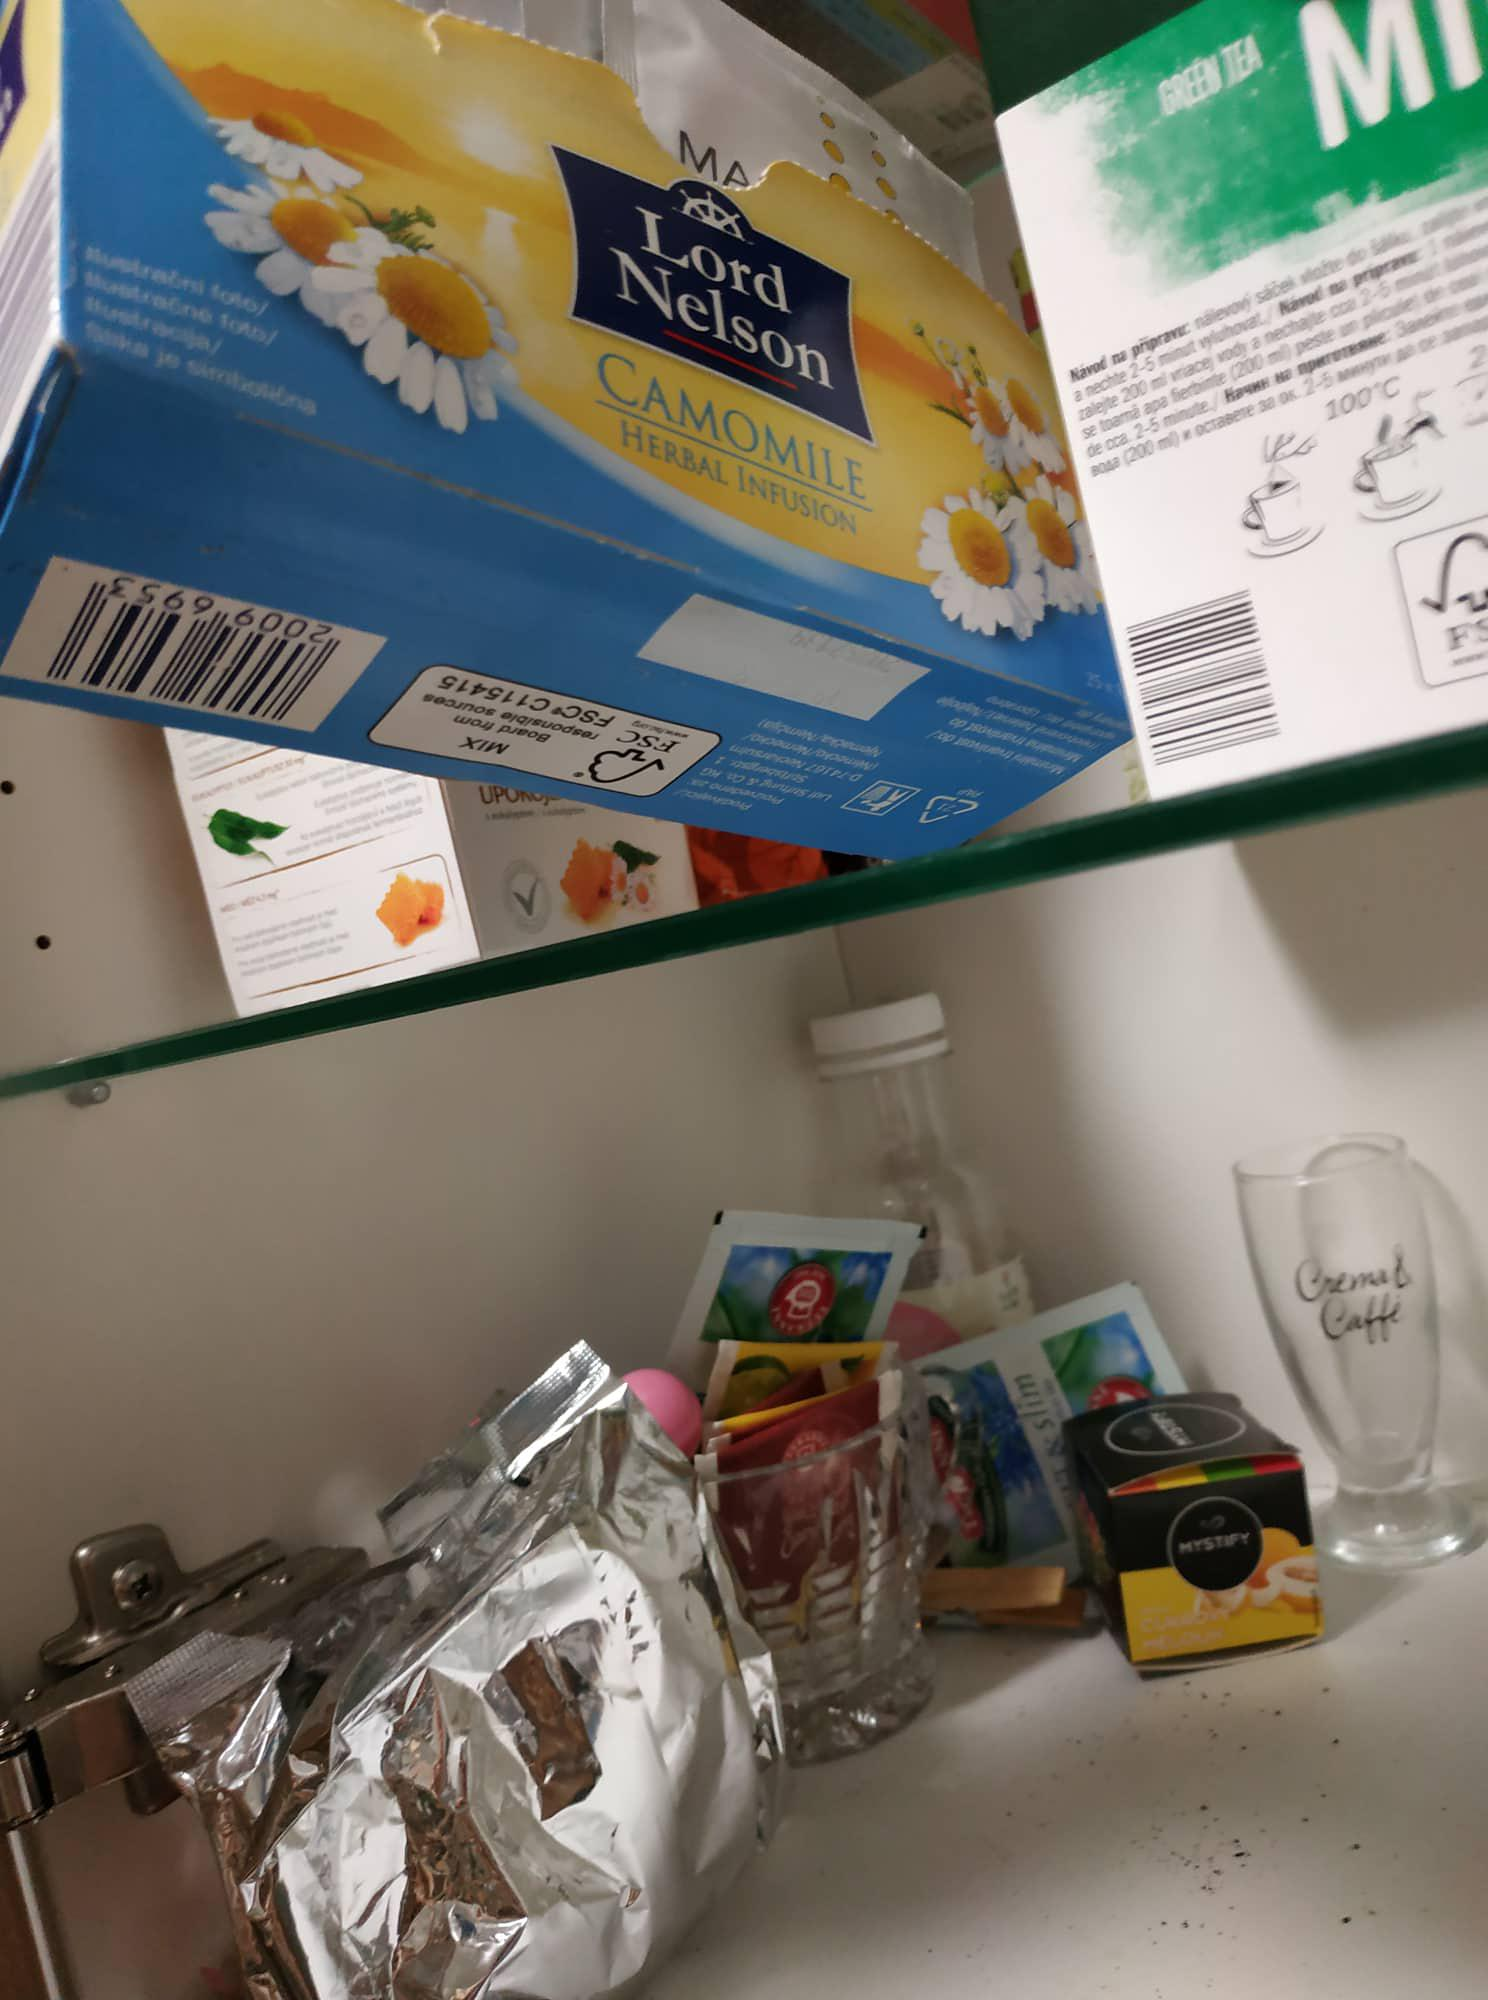
\includegraphics[width=0.41\linewidth]{obrazky-figures/merge_implement.jpg}\hfill
    \caption{Původní obrázek}
    \end{subfigure}
    \begin{subfigure}{0.6\textwidth}
    \fbox{\includegraphics[width=0.4\linewidth]{obrazky-figures/blank_1_merge_implement.jpg}}\hfill
    \includegraphics[width=0.41\linewidth]{obrazky-figures/sub_final_1_merge_implement.jpg}\hfill
    \caption{První výřez vložený do prázdného obrázku. Detektor v něm detekoval čárový kód a vložil jej do původního obrázku.}
    \end{subfigure}
    \begin{subfigure}{0.6\textwidth}
    \fbox{\includegraphics[width=0.4\linewidth]{obrazky-figures/blank_2_merge_implement.jpg}}\hfill
    \includegraphics[width=0.41\linewidth]{obrazky-figures/sub_final_2_merge_implement.jpg}\hfill
    \caption{Detektoru se nepodařilo detekovat čárový kód v druhém výřezu, vložil tedy do původního obrázku, ve kterém již byl ohraničující box z prvního výřezu, ohraničující box samotného výřezu.}
    \end{subfigure}
    \caption{Postupná detekce čárových kódů v obraze.}
    \label{merge_implement}
\end{figure}
\clearpage

\paragraph{} Poté probíhá samotná detekce čárového kódu ve výřezu pomocí detektoru čárových kódů knihovny OpenCV. Nejprve se vygeneruje prázdný obrázek, do kterého se na detekované souřadnice vloží výřezek čárového kódu. Tímto se zabrání přebytečnému šumu a omezí se počet false positives. Následně se zavolá funkce \texttt{detectAndDecode\char`(\char`)} třídy čárového detektoru knihovy OpenCV, která detekuje čárový kód a zároveň jej dekóduje. Pokud se funkce detekovala čárový kód, zakreslí se do výstupního obrázku a zapíše se do řetězce \texttt{detected\char`_boxes\char`(\char`)}, jenž bude později využit pro počítání metrik. Díky tomu že byl výřezek vložen do obrázku, sedí souřadnice detekovaného čárového kódu s původní obrázkem, ohraničující box jde tedy zakreslit bez jakéhokoliv přepočtu souřadnic. Zároveň pokud je úspěšné i dekódování čárového kódu, připočítá se do integeru \texttt{decoded}. Pokud však žádný čárový kód není detekován, vezme se místo něj čárový kód detekovaný sítí YOLOv5, jelikož má lepší recall než metoda knihovny OpenCV jak lze vidět v tabulkách \ref{opencv_table} a \ref{yolov5_table}. Toto probíhá pro všechny detekované čárové kódy v obrázku.


\paragraph{} Nakonec detekce se vykreslí výsledný obrázek s detekovanými čárovými kódy, a spočítá čas který detekce celého obrázku zabrala. Poté se už jen zavolá funkce \texttt{calculate\char`_ious\char`(\char`)}, která slouží na výpočet hodnot intersection over union, jejíž výsledek se zapíše do řetezce hodnot intersection over union všech detekovaných čárových kódů. Tím končí detekce jednoho obrázku a cyklus se opakuje pro zbytek obrázků. Příklad detekce čárových kódu jednoho obrázku jde vidět v obrázku \ref{merge_implement}.
\subsection*{Počítání metrik}
\paragraph{} Pokud bylo detekováno méně ohraničujících boxů, než kolik jich bylo předem definováno, za každý takto nedetekovaný ohraničující box se vrací -1, což indikuje false negative. Funkce \texttt{calculate\char`_ious\char`(\char`)} cyklí přes všechny předem definované ohraničující boxy v obraze. V každém tomto cyklu cyklí ještě přes všechny detekované ohraničující boxy. Nejprve zde získáme rohy obou ohraničujících boxů, pomocí kterých vypočítáme oblast průniku a oblast sjednocení. Tyto oblasti program počítá pomocí knihovny \texttt{shapely}. Poté už jen vypočítáme intersection over union vydělením těchto dvou oblastí.
\paragraph{} Protože program počítá intersection union pro každou dvojici ohraničujících boxů, musí toto číslo zredukovat na počet detekovaných ohraničujících boxů. Toto se udělá pomocí funkce příkazu \texttt{np.argsort\char`(ious\char`)\char`[-len(detected\char`_boxes):\char`]}, kde \texttt{np} představuje knihovnu \texttt{numpy}. Tento příkaz vrátí stejný počet indexů hodnot intersection over union jako je počet detekovaných ohraničujících boxů. Tyto indexy ukazují na největší vypočítané hodnoty, které poté funkce vrací.
\paragraph{} Na úplném konci programu se volá funkce \texttt{calculate\char`_mAP\char`(\char`)} pro různé prahy, konkrétně tedy 0.5, 0.75 a 0.9. V této funkci se nejprve rozdělí všechny hodnoty intersection over union na false negatives, true positives a false positives. Pokud je hodnota -1, klasifikuje se jako false negative. Pokud je hodnota větší než daný práh, je true positive a jinak je false positive. Tyto klasifikace se sčítají. Pomocí těchto klasifikací můžeme vypočítat hodnoty precision, recall a f1 (sekce \ref{prf}) a average precision (sekce \ref{ap}).
\paragraph{} Program používá také několik pomocných funkcí. Funkce \texttt{relative\char`_to\char`_absolute\char`_coords\char`(\char`)} vezme na vstupu relativní souřadnice ohraničujícího boxu a šířku a výšku obrázku. Tyto souřadnice poté převede na absolutní souřadnice. Funkce \texttt{bbox\char`_to\char`_points\char`(\char`)} převede ohraničující box ve formátu \texttt{class, xcenter, ycenter, width, height} na formát \texttt{x1, y1, x2, y2, x3, y3, x4, y4}, aby byl kompatibilní s orientovanými ohraničujícími boxy. \linebreak Funkce \texttt{change\char`_file\char`_format\char`(\char`)} převádí formát názvu souboru například z \texttt{.jpg} na \texttt{.txt} a funkce \texttt{file\char`_to\char`_array\char`_list\char`(\char`)} převede všechny štítky z souboru se štítky na řetězec, který následně vrací.



\section{Zhodnocení navržené metody}
\label{final_eval}
\paragraph{} Navržená metoda používá nejlepší váhy natrénované v sekci \ref{opencv_exp}. Na datasetu popsaném v kapitole \ref{dataset}. Testování probíhalo pro celý dataset, aliasovanou část a nealiasovanou část s prahy 0.5, 0.75 a 0.9. Naměřené hodnoty metrik lze vidět v tabulce \ref{merge_table}.
\paragraph{} Při testování na celém datasetu dosáhla navržená metoda při prahu 0.5 average precision 0.6966, což je mírné zlepšení oproti 0.6624 metody YOLOv5 a znatelné zlepšení oproti detektoru čárových kódů knihovny OpenCV s hodnotou 0.3128 (graf \ref{thresh-0.5}). Nepatrně se zlepšila také hodnota metriky recall a to z 0.9811 metody YOLOv5 a 0.3818 detektoru knihovny OpenCV. Hodnota recall navržené metody je 0.9826. Metoda tedy velmi dobře dokáže detekovat pozitivní vzorky. Precision navržené metody je 0.7663 což je mírné zlepšení oproti precision metody YOLOv5 s hodnotou 0.7287. Avšak v porovnání s detektorem knihovny OpenCV navržená metoda poněkud pokulhává. Ten měl hodnotu precision 0.8603, což je však dáno nižším počtem detekovaných čárových kódů. Hodnota F1 0.8611 je zlepšením oproti oběma metodám s hodnotami 0.8362 pro YOLOv5 a 0.5289 pro detektor OpenCV.

\paragraph{} Podobné zlepšení lze pozorovat i u aliasované a nealiasované části datasetu, je však mnohem výraznější u nealiasované části. Tam je hodnota average precision 0.7574 oproti 0.7035 metody YOLOv5 a 0.5037 detektoru OpenCV. Podobně je to také se zbytkem měřených metrik. Recall byl spočítán jako 0.9933 a precision jako 0.8331. Skóre F1 dosáhlo hodnoty 0.9062. Což je opět zlepšení oproti hodnotám YOLOv5 (recall je 0.9919, precision 0.7739 a F1 0.9061) a hodnotám detektoru knihovny OpenCV (recall je 0.5004, precision 0.9234 a F1 0.639).

\paragraph{} U aliasovaných části datasetu je zlepšení oproti YOLOv5 méně znatelné. Average precision navržené metody na aliasované části datasetu je 0.5997, recall 0.9615, precision 0.6596 a skóre F1 0.7825. YOLOv5 dosahuje podobných hodnot, kde average precision je 0.5967, recall 0.9612, precision 0.6564 a skóre F1 0.7801. Naproti tomu je to výrazným zlepšením oproti detektoru knihovny OpenCV, který má s aliasovanými vstupy problémy. Average precision tohoto detektoru je 0.1114, recall 0.1591, precision 0.6128 a skóre F1 je 0.2526.

`
\begin{figure}[h]
  \centering
  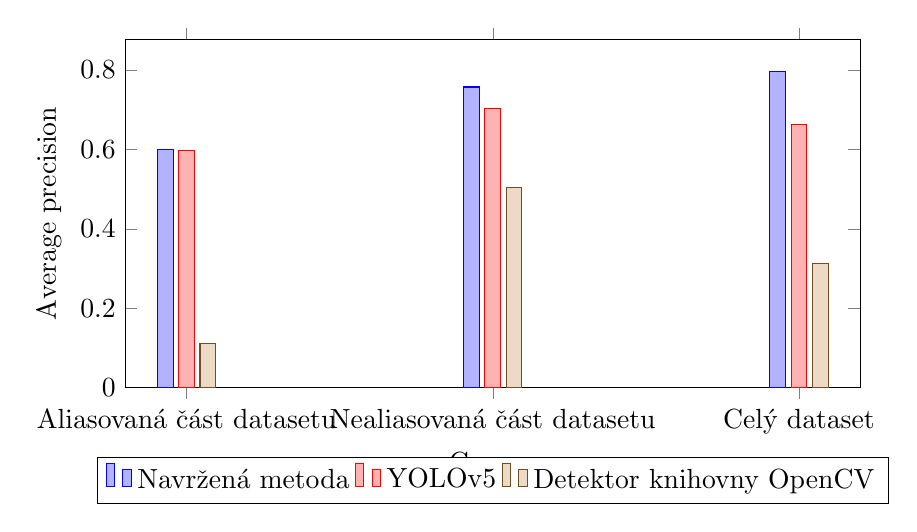
\begin{tikzpicture}
    \begin{axis}[
      ybar,
      ymin=0,
      width=0.9\textwidth,
      height=6cm,
      bar width=0.2cm,
      xtick=data,
      xticklabels={Aliasovaná část datasetu, Nealiasovaná část datasetu, Celý dataset},
      xlabel={Groups},
      ylabel={Average precision},
      legend entries={Navržená metoda, YOLOv5, Detektor knihovny OpenCV},
      legend style={at={(0.5,-0.2)},
      anchor=north,legend columns=-1},
      ]
      \addplot coordinates {(1,0.5996) (2,0.7574) (3,0.7966)};
      \addplot coordinates {(1,0.5967) (2,0.7035) (3,0.6624)};
      \addplot coordinates {(1,0.1114) (2,0.5037) (3,0.3128)};
    \end{axis}
  \end{tikzpicture}
  \caption{Porovnání hodnot average precision metod s prahem 0.5}
  \label{thresh-0.5}
\end{figure}
\pagebreak

\paragraph{} Při zvyšujícím se prahu však efektivita navržené metody, v porovnání s metodou YOLOv5, znatelně klesá (graf \ref{thresh-0.75}). Je to dáno zejména špatnou efektivitou detektoru knihovny OpenCV při vyšších hodnotách prahu. Navržená metoda má s prahem 0.75 na celém datasetu average precision 0.2073, recall 0.9437, precision 0.2281 a skóre F1 0.3673. Naproti tomu metoda YOLOv5 má average precision 0.3056, recall 0.9598, precision 0.3362 a skóre F1 0.4979. Jak již bylo zmíněno detektor knihovny OpenCV má na vyšším prahu velmi špatnou schopnost detekce. Jeho average precision je pouze 0.0393, recall 0.1344, precision 0.2162 a skóre F1 je 0.1657.


\paragraph{} U aliasované a nealisované části datasetu na prahu 0.75 jsou změny obdobné. Navržená metoda má při testování na aliasované části datasetu hodnotu average precision 0.1643, recall 0.8838, precision 0.2009 a skóre F1 0.3273. Nealiasovaná část má average precision 0.2228, recall 0.9777, precision 0.2451 a F1 0.3919. V porovnání s metodou YOLOv5 je zhoršení poměrově stejné jako u celého datasetu.

\begin{figure}[h]
  \centering
  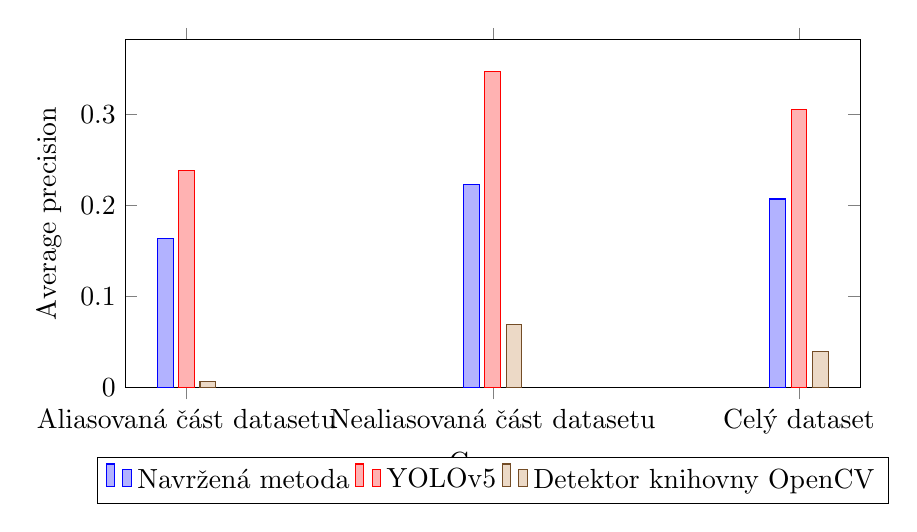
\begin{tikzpicture}
    \begin{axis}[
      ybar,
      ymin=0,
      width=0.9\textwidth,
      height=6cm,
      bar width=0.2cm,
      xtick=data,
      xticklabels={Aliasovaná část datasetu, Nealiasovaná část datasetu, Celý dataset},
      xlabel={Groups},
      ylabel={Average precision},
      legend entries={Navržená metoda, YOLOv5, Detektor knihovny OpenCV},
      legend style={at={(0.5,-0.2)},
      anchor=north,legend columns=-1},
      ]
      \addplot coordinates {(1,0.1643) (2,0.2228) (3,0.2073)};
      \addplot coordinates {(1,0.2388) (2,0.3475) (3,0.3056)};
      \addplot coordinates {(1,0.0063) (2,0.0692) (3,0.0393)};
    \end{axis}
  \end{tikzpicture}
  \caption{Porovnání hodnot average precision metod s prahem 0.75}
  \label{thresh-0.75}
\end{figure}

\paragraph{} S prahem 0.9 nastává další propad (graf \ref{thresh-0.9}). Average precision navržené metody na celém datasetu je 0.0323, recall je 0.7654, precision 0.0444 a F1 0.0839. Což znamená že na vyších hodnotách prahu je tato metoda v podstatě nepoužitelná. Stejný propad lze pozorovat i u aliasované a nealiasované části datasetu. Aliasovaná část má hodnotu average precision 0.0214, recall 0.5978, precision 0.03924 a F1 0.07365. Nealiasovaná má average precision rovnu 0.03893, recall 0.8949, precision  0.0476 a F1 0.09036.

\begin{figure}[h]
  \centering
  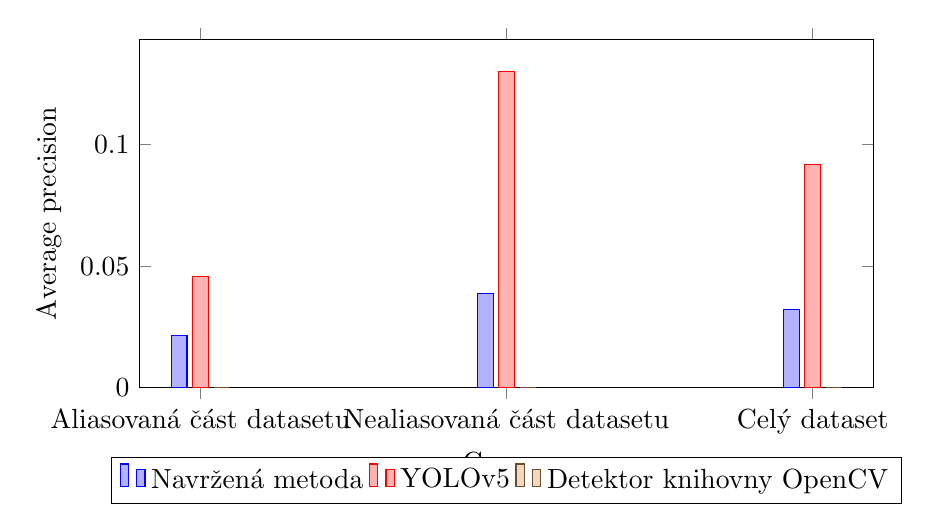
\begin{tikzpicture}
    \begin{axis}[
      ybar,
      ymin=0,
      width=0.9\textwidth,
      height=6cm,
      bar width=0.2cm,
      xtick=data,
      xticklabels={Aliasovaná část datasetu, Nealiasovaná část datasetu, Celý dataset},
      xlabel={Groups},
      ylabel={Average precision},
      legend entries={Navržená metoda, YOLOv5, Detektor knihovny OpenCV},
      legend style={at={(0.5,-0.2)},
      anchor=north,legend columns=-1},
      ytick={0, 0.05, 0.1},
      yticklabels={0, 0.05, 0.1},
      ]
      \addplot coordinates {(1,0.0214) (2,0.0389) (3,0.0323)};
      \addplot coordinates {(1,0.0456) (2,0.1301) (3,0.0918)};
      \addplot coordinates {(1,0) (2,0) (3,0)};
    \end{axis}
  \end{tikzpicture}
  \caption{Porovnání hodnot average precision metod s prahem 0.9}
  \label{thresh-0.9}
\end{figure}
\pagebreak
\paragraph{} Díky použití detektoru knihovny OpenCV, má tato metoda také schopnost dekódovat čárové kódy. Na celém datasetu se podařilo dekódovat 36.97\% detekovaných čárových kódů. Při použití pouze detektoru OpenCV je míra dekódování 41.79\%. Což je dáno zejména menším počtem detekovaným čárových kódů detektorem OpenCV. V absolutích číslech je však detekce také horší. Navrhovaná metoda dekódovala pouze 2728 čárových kódů, zatímco samotný detektor OpenCV jich dekódoval 2770. Bez kontextu bezprostředního okolí čárového kódu je míra dekódování zřejmě menší.

\begin{table}[ht]
\centering
\begin{tabular}{|l|c|c|c|c|}
\hline
Práh - dataset     & Average precision & Recall  & Precision & F1      \\ \hline
0.5 - aliased & 0.5996 & \multicolumn{1}{l|}{0.9615} & \multicolumn{1}{l|}{ 0.6597} & \multicolumn{1}{l|}{0.7825} \\ \hline
0.5 - not aliased  & 0.7574           & 0.9933 & 0.8331   & 0.9062 \\ \hline
0.5 - combined     & 0.7966          & 0.9826 & 0.7663    & 0.8611 \\ \hline
0.75 - aliased     & 0.1643             & 0.8838  & 0.2009    & 0.3273  \\ \hline
0.75 - not aliased & 0.2228            & 0.9777 & 0.2451   & 0.3919 \\ \hline
0.75 - combined    & 0.2073            & 0.9437 & 0.2281   & 0.3673  \\ \hline
0.9 - aliased      & 0.0214              & 0.5978     & 0.0392       & 0.0737     \\ \hline
0.9 - not aliased  & 0.0389               & 0.8949     & 0.0476       & 0.0904     \\ \hline
0.9 - combined     & 0.0323               & 0.7654     & 0.0444       & 0.0839     \\ \hline
\end{tabular}
\caption{V této tabulce jsou přehledně zapsány naměřené metriky navržené metody detekce čárových kódů.}
\label{merge_table}
\end{table}


\chapter{Závěr}
\label{zaver}
Cílem této práce bylo porovnat existující metody detekce čárových kódů v obraze a navrhnout a implementovat vylepšení některé z těchto metod. 

V této práci jsem sepsal základní informace o čárových kódech a jejich rozdělení. Popsal jsem také různé metody detekce objektů v obraze od detekce hran po neuronové sítě. Tři z těchto metod, konkrétně Scharrovu metodu, detektor knihovny OpenCV a umělou neuronovou síť YOLOv5 jsem otestoval na rozsáhlém datasetu. Změřil jsem také vliv aliasingu na jednotlivé metody detekce čárových kódů.

Poté jsem navrhnul a implementoval metodu pro detekci čárových kódů, která byla kombinací metody YOLOv5 a detektoru knihovny OpenCV. Podařilo se mi zvýšit kvalitu detekce oproti testovaným metodám při hodnotách prahu 0.5. Navržená metoda dosáhla zvýšení metriky average precision o 3.42\% oproti metodě YOLOv5 a 38.38\% oproti detektoru knihovny OpenCV. Při vyšších hodnotách prahu je naržené řešení bohužel znatelně horší než samotná metoda YOLOv5. Což je způsobeno špatným výkonem detektoru knihovny OpenCV při vyšších hodnotách prahu.

Práce by v budoucnu mohla být rozšířena o více testovaných metod, jak neuronových sítí, tak metod založených na pravidlech. V této práci jsem testoval pouze single shot metodu YOLOv5, bylo by tedy vhodné otestovat také některou z two shot neuronových sítí. Také by se mohlo otestovat více metod založených na pravidlech, konkrétně tedy Harrisův detektor rohů nebo metodu detekce Curvature Scale Space popsané v kapitolách \ref{detekce_rohu}. To by mohlo vést k nalezení vhodnějších metod pro samotnou kombinaci.







%===============================================================================

% Pro kompilaci po částech (viz projekt.tex) nutno odkomentovat
%\end{document}
